% Options for packages loaded elsewhere
\PassOptionsToPackage{unicode}{hyperref}
\PassOptionsToPackage{hyphens}{url}
%
\documentclass[
]{article}
\title{Gráficos con R}
\author{Olivier Nuñez}
\date{2022-05-09}

\usepackage{amsmath,amssymb}
\usepackage{lmodern}
\usepackage{iftex}
\ifPDFTeX
  \usepackage[T1]{fontenc}
  \usepackage[utf8]{inputenc}
  \usepackage{textcomp} % provide euro and other symbols
\else % if luatex or xetex
  \usepackage{unicode-math}
  \defaultfontfeatures{Scale=MatchLowercase}
  \defaultfontfeatures[\rmfamily]{Ligatures=TeX,Scale=1}
\fi
% Use upquote if available, for straight quotes in verbatim environments
\IfFileExists{upquote.sty}{\usepackage{upquote}}{}
\IfFileExists{microtype.sty}{% use microtype if available
  \usepackage[]{microtype}
  \UseMicrotypeSet[protrusion]{basicmath} % disable protrusion for tt fonts
}{}
\makeatletter
\@ifundefined{KOMAClassName}{% if non-KOMA class
  \IfFileExists{parskip.sty}{%
    \usepackage{parskip}
  }{% else
    \setlength{\parindent}{0pt}
    \setlength{\parskip}{6pt plus 2pt minus 1pt}}
}{% if KOMA class
  \KOMAoptions{parskip=half}}
\makeatother
\usepackage{xcolor}
\IfFileExists{xurl.sty}{\usepackage{xurl}}{} % add URL line breaks if available
\IfFileExists{bookmark.sty}{\usepackage{bookmark}}{\usepackage{hyperref}}
\hypersetup{
  pdftitle={Gráficos con R},
  pdfauthor={Olivier Nuñez},
  hidelinks,
  pdfcreator={LaTeX via pandoc}}
\urlstyle{same} % disable monospaced font for URLs
\usepackage[margin=1in]{geometry}
\usepackage{color}
\usepackage{fancyvrb}
\newcommand{\VerbBar}{|}
\newcommand{\VERB}{\Verb[commandchars=\\\{\}]}
\DefineVerbatimEnvironment{Highlighting}{Verbatim}{commandchars=\\\{\}}
% Add ',fontsize=\small' for more characters per line
\usepackage{framed}
\definecolor{shadecolor}{RGB}{248,248,248}
\newenvironment{Shaded}{\begin{snugshade}}{\end{snugshade}}
\newcommand{\AlertTok}[1]{\textcolor[rgb]{0.94,0.16,0.16}{#1}}
\newcommand{\AnnotationTok}[1]{\textcolor[rgb]{0.56,0.35,0.01}{\textbf{\textit{#1}}}}
\newcommand{\AttributeTok}[1]{\textcolor[rgb]{0.77,0.63,0.00}{#1}}
\newcommand{\BaseNTok}[1]{\textcolor[rgb]{0.00,0.00,0.81}{#1}}
\newcommand{\BuiltInTok}[1]{#1}
\newcommand{\CharTok}[1]{\textcolor[rgb]{0.31,0.60,0.02}{#1}}
\newcommand{\CommentTok}[1]{\textcolor[rgb]{0.56,0.35,0.01}{\textit{#1}}}
\newcommand{\CommentVarTok}[1]{\textcolor[rgb]{0.56,0.35,0.01}{\textbf{\textit{#1}}}}
\newcommand{\ConstantTok}[1]{\textcolor[rgb]{0.00,0.00,0.00}{#1}}
\newcommand{\ControlFlowTok}[1]{\textcolor[rgb]{0.13,0.29,0.53}{\textbf{#1}}}
\newcommand{\DataTypeTok}[1]{\textcolor[rgb]{0.13,0.29,0.53}{#1}}
\newcommand{\DecValTok}[1]{\textcolor[rgb]{0.00,0.00,0.81}{#1}}
\newcommand{\DocumentationTok}[1]{\textcolor[rgb]{0.56,0.35,0.01}{\textbf{\textit{#1}}}}
\newcommand{\ErrorTok}[1]{\textcolor[rgb]{0.64,0.00,0.00}{\textbf{#1}}}
\newcommand{\ExtensionTok}[1]{#1}
\newcommand{\FloatTok}[1]{\textcolor[rgb]{0.00,0.00,0.81}{#1}}
\newcommand{\FunctionTok}[1]{\textcolor[rgb]{0.00,0.00,0.00}{#1}}
\newcommand{\ImportTok}[1]{#1}
\newcommand{\InformationTok}[1]{\textcolor[rgb]{0.56,0.35,0.01}{\textbf{\textit{#1}}}}
\newcommand{\KeywordTok}[1]{\textcolor[rgb]{0.13,0.29,0.53}{\textbf{#1}}}
\newcommand{\NormalTok}[1]{#1}
\newcommand{\OperatorTok}[1]{\textcolor[rgb]{0.81,0.36,0.00}{\textbf{#1}}}
\newcommand{\OtherTok}[1]{\textcolor[rgb]{0.56,0.35,0.01}{#1}}
\newcommand{\PreprocessorTok}[1]{\textcolor[rgb]{0.56,0.35,0.01}{\textit{#1}}}
\newcommand{\RegionMarkerTok}[1]{#1}
\newcommand{\SpecialCharTok}[1]{\textcolor[rgb]{0.00,0.00,0.00}{#1}}
\newcommand{\SpecialStringTok}[1]{\textcolor[rgb]{0.31,0.60,0.02}{#1}}
\newcommand{\StringTok}[1]{\textcolor[rgb]{0.31,0.60,0.02}{#1}}
\newcommand{\VariableTok}[1]{\textcolor[rgb]{0.00,0.00,0.00}{#1}}
\newcommand{\VerbatimStringTok}[1]{\textcolor[rgb]{0.31,0.60,0.02}{#1}}
\newcommand{\WarningTok}[1]{\textcolor[rgb]{0.56,0.35,0.01}{\textbf{\textit{#1}}}}
\usepackage{longtable,booktabs,array}
\usepackage{calc} % for calculating minipage widths
% Correct order of tables after \paragraph or \subparagraph
\usepackage{etoolbox}
\makeatletter
\patchcmd\longtable{\par}{\if@noskipsec\mbox{}\fi\par}{}{}
\makeatother
% Allow footnotes in longtable head/foot
\IfFileExists{footnotehyper.sty}{\usepackage{footnotehyper}}{\usepackage{footnote}}
\makesavenoteenv{longtable}
\usepackage{graphicx}
\makeatletter
\def\maxwidth{\ifdim\Gin@nat@width>\linewidth\linewidth\else\Gin@nat@width\fi}
\def\maxheight{\ifdim\Gin@nat@height>\textheight\textheight\else\Gin@nat@height\fi}
\makeatother
% Scale images if necessary, so that they will not overflow the page
% margins by default, and it is still possible to overwrite the defaults
% using explicit options in \includegraphics[width, height, ...]{}
\setkeys{Gin}{width=\maxwidth,height=\maxheight,keepaspectratio}
% Set default figure placement to htbp
\makeatletter
\def\fps@figure{htbp}
\makeatother
\setlength{\emergencystretch}{3em} % prevent overfull lines
\providecommand{\tightlist}{%
  \setlength{\itemsep}{0pt}\setlength{\parskip}{0pt}}
\setcounter{secnumdepth}{5}
\usepackage[spanish]{babel}
\selectlanguage{spanish}

\usepackage{xcolor}
\usepackage[framemethod=default]{mdframed}


\newcounter{ejcnt}[section]
\numberwithin{ejcnt}{section}

%\newenvironment{nota}
%{ \rule{1ex}{1ex}\hspace{\stretch{1}} }
%{ \hspace{\stretch{1}}\rule{1ex}{1ex} }


\global\mdfdefinestyle{exampledefault}{%
linecolor=lightgray,linewidth=1pt,%
leftmargin=1cm,rightmargin=1cm,
}

%\newenvironment{nota}[1]{%
\newenvironment{nota}{%
\mdfsetup{%
frametitle={\colorbox{white}{\,Nota\,}},
%frametitle={\colorbox{white}{\,#1\,}},
frametitleaboveskip=-\ht\strutbox,
frametitlealignment=\raggedright
}%
\begin{mdframed}[style=exampledefault]
}{\end{mdframed}}

\newenvironment{rien}{%
\begin{mdframed}[style=exampledefault]
}{\end{mdframed}}



\newenvironment{ej}[1][]{%
	\refstepcounter{ejcnt}%
	\par\medskip%
	\noindent% 
	\textbf{Ejercicio \theejcnt \;\;}% 
	\rmfamily%
}{\medskip}


%\newenvironment{ej}[1][]{\refstepcounter{ej}\par\medskip
%   \noindent \textbf{Ejercicio #1} \rmfamily}{\medskip}

%\newenvironment{ej}% environment name
%{% begin code
%  \par\vspace{\baselineskip}\noindent
%  \leftmargin=0.3in\rightmargin=0.3in
%  \textbf{Ejercicio:}
%  %\par\vspace{\baselineskip}\noindent\ignorespaces
%}%
%{% end code
%  \ignorespacesafterend
%}

%\makeatletter
%\renewcommand{\subsubsection}{\ttl@straightclass{subsubsection}}
%\makeatother
%\titleformat{\subsubsection}[hang]
%  {\fontsize{36}{42}\selectfont}
%  {\thesubsubsection}
%  {1em}
%  {}
%  []
\ifLuaTeX
  \usepackage{selnolig}  % disable illegal ligatures
\fi
\usepackage[]{natbib}
\bibliographystyle{plainnat}

\begin{document}
\maketitle

{
\setcounter{tocdepth}{2}
\tableofcontents
}
\hypertarget{preuxe1mbulo}{%
\section*{Preámbulo}\label{preuxe1mbulo}}
\addcontentsline{toc}{section}{Preámbulo}

\begin{quote}
``Una imagen vale más que mil palabras'' (``Un bon croquis vaut mieux qu'un long discours'')

--- Napoleon
\end{quote}

\begin{itemize}
\item
  La representación gráfica de los datos es una potente herramienta de síntesis de la información estadística.
\item
  Cualquiera que sea la etapa de su trabajo (exploración, modelización, confirmación o comunicación de resultados), el usuario de métodos estadísticos encuentra en los gráficos un aliado para ahorrar tiempo.
\item
  El objetivo de esta sesión es manejar el paquete \texttt{ggplot2} de R y sus extensiones que permiten un diseño eficiente de gráficos para explorar la distribución de un conjunto de datos. Se abordarán los distintos pasos, que van desde la preparación de los datos hasta su exportación.
\item
  La estructura de esta sesión tiene tres partes:

  \begin{itemize}
  \tightlist
  \item
    La primera parte está dedicada a la definición y elaboración de las representaciones gráficas más comunes (diagrama de barras, de caja, de dispersión, histograma) para extraer la información contenida en un conjunto de datos.
  \item
    La segunda parte describe la ``gramática'' general de confección de gráficos utilizada en \texttt{ggplot2}. Esta gramática permite tratar de manera sistemática y flexible, aspectos básicos como la elección de los ejes, los colores y la leyenda. Pero también, temas avanzados como el problema de solapamiento de puntos, la superposición de varios elementos gráficos (capas) o el desglose de una representación en varios sub-gráficos (facetas).
  \item
    En la ultima parte, se presentarán una extensión de \texttt{R} para insertar esta información gráfica en informes automatizados, mediante el paquete \texttt{Rmarkdown}.
  \end{itemize}
\end{itemize}

\hypertarget{gruxe1ficos-buxe1sicos-en-el-anuxe1lisis-de-datos}{%
\section{Gráficos básicos en el análisis de datos}\label{gruxe1ficos-buxe1sicos-en-el-anuxe1lisis-de-datos}}

Esta sección es una breve introducción a los gráficos más comunes para analizar conjuntos de datos. Para ello, utilizaremos el paquete \texttt{ggplot2} (``gg'' para ``Grammar of Graphics'').

\begin{Shaded}
\begin{Highlighting}[]
\CommentTok{\#install.packages("ggplot2")}
\FunctionTok{library}\NormalTok{(ggplot2) }\CommentTok{\#carga la librería ggplot2}
\end{Highlighting}
\end{Shaded}

Empezaremos con la función básica \texttt{qplot}(``quick plot'') de este paquete. Una descripción abreviada de esta función es

\begin{Shaded}
\begin{Highlighting}[]
\FunctionTok{qplot}\NormalTok{(x, }\AttributeTok{y=}\ConstantTok{NULL}\NormalTok{, data, }\AttributeTok{geom=}\StringTok{"auto"}\NormalTok{, }\AttributeTok{xlim =} \FunctionTok{c}\NormalTok{(}\ConstantTok{NA}\NormalTok{, }\ConstantTok{NA}\NormalTok{), }\AttributeTok{ylim =}\FunctionTok{c}\NormalTok{(}\ConstantTok{NA}\NormalTok{, }\ConstantTok{NA}\NormalTok{))}
\end{Highlighting}
\end{Shaded}

\begin{nota}
\begin{itemize}
\tightlist
\item
  \texttt{x} : valores en el eje de abscisas.
\item
  \texttt{y} : valores en el de ordenadas (opcional).
\item
  \texttt{data} : data.frame de donde salen los datos (opcional).
\item
  \texttt{geom} : elementos gráficos o geometrías
  (``point'',line'',``bar'',\ldots). Por defecto, ``point'' si
  \texttt{y} viene especificado, e ``histogram'' si sólo se especifica
  \texttt{x}.
\item
  \texttt{xlim}, \texttt{ylim}: limites en los ejes de \texttt{x} e
  \texttt{y}.
\end{itemize}

Otros argumentos relacionados con los ejes y el titulo del gráfico son:
\texttt{main}: titulo del gráfico; \texttt{xlab}, \texttt{ylab}:
etiquetas los los ejes; \texttt{log}: ejes en escala log. Los valores
permitidos son ``x'', ``y'' o bien ``xy''.
\end{nota}

\hypertarget{distribuciuxf3n-de-una-variable}{%
\subsection{Distribución de una variable}\label{distribuciuxf3n-de-una-variable}}

Para intentar ver algo en un conjunto de datos, lo primero que se puede hacer es averiguar como se distribuyen sus valores. En R, hay funciones básicas (summary, stem, table, \ldots) que permiten tener una idea de esta distribución.

El tipo de representación gráfica de la distribución cambia según la naturaleza de la variable en estudio. Una variable cuantitativa toma valores numéricos. Para una variable cuantitativa, se suele recurrir a un \textbf{histograma} o bien a un \textbf{diagrama de caja} para describir su distribución. Mientras que para variables cualitativas (o categóricas), se utilizará un \emph{diagrama de barras}.

\hypertarget{histograma}{%
\subsubsection{Histograma}\label{histograma}}

Para ilustrar la descripción gráfica de la distribución de una variable numérica, se utiliza la base de datos \texttt{msleep} que contiene información sobre el tiempo de sueño (en horas) de mamíferos:

\begin{Shaded}
\begin{Highlighting}[]
\NormalTok{msleep }\CommentTok{\# ?msleep para más detalles}
\end{Highlighting}
\end{Shaded}

\begin{verbatim}
## # A tibble: 83 x 11
##    name                       genus       vore  order conservation sleep_total sleep_rem sleep_cycle awake  brainwt  bodywt
##    <chr>                      <chr>       <chr> <chr> <chr>              <dbl>     <dbl>       <dbl> <dbl>    <dbl>   <dbl>
##  1 Cheetah                    Acinonyx    carni Carn~ lc                  12.1      NA        NA      11.9 NA        50    
##  2 Owl monkey                 Aotus       omni  Prim~ <NA>                17         1.8      NA       7    0.0155    0.48 
##  3 Mountain beaver            Aplodontia  herbi Rode~ nt                  14.4       2.4      NA       9.6 NA         1.35 
##  4 Greater short-tailed shrew Blarina     omni  Sori~ lc                  14.9       2.3       0.133   9.1  0.00029   0.019
##  5 Cow                        Bos         herbi Arti~ domesticated         4         0.7       0.667  20    0.423   600    
##  6 Three-toed sloth           Bradypus    herbi Pilo~ <NA>                14.4       2.2       0.767   9.6 NA         3.85 
##  7 Northern fur seal          Callorhinus carni Carn~ vu                   8.7       1.4       0.383  15.3 NA        20.5  
##  8 Vesper mouse               Calomys     <NA>  Rode~ <NA>                 7        NA        NA      17   NA         0.045
##  9 Dog                        Canis       carni Carn~ domesticated        10.1       2.9       0.333  13.9  0.07     14    
## 10 Roe deer                   Capreolus   herbi Arti~ lc                   3        NA        NA      21    0.0982   14.8  
## # ... with 73 more rows
\end{verbatim}

\begin{Shaded}
\begin{Highlighting}[]
\CommentTok{\#summary(msleep$sleep\_total) \#tiempo total de sueño (en horas)}
\FunctionTok{stem}\NormalTok{(msleep}\SpecialCharTok{$}\NormalTok{sleep\_total)}
\end{Highlighting}
\end{Shaded}

\begin{verbatim}
## 
##   The decimal point is at the |
## 
##    0 | 9
##    2 | 79013589
##    4 | 0423346
##    6 | 23307
##    8 | 03446779114456788
##   10 | 01113346900135
##   12 | 15555880578
##   14 | 234456996889
##   16 | 604
##   18 | 01479
\end{verbatim}

\begin{Shaded}
\begin{Highlighting}[]
\FunctionTok{qplot}\NormalTok{(sleep\_total,}\AttributeTok{data=}\NormalTok{msleep) }\CommentTok{\#histograma }
\end{Highlighting}
\end{Shaded}

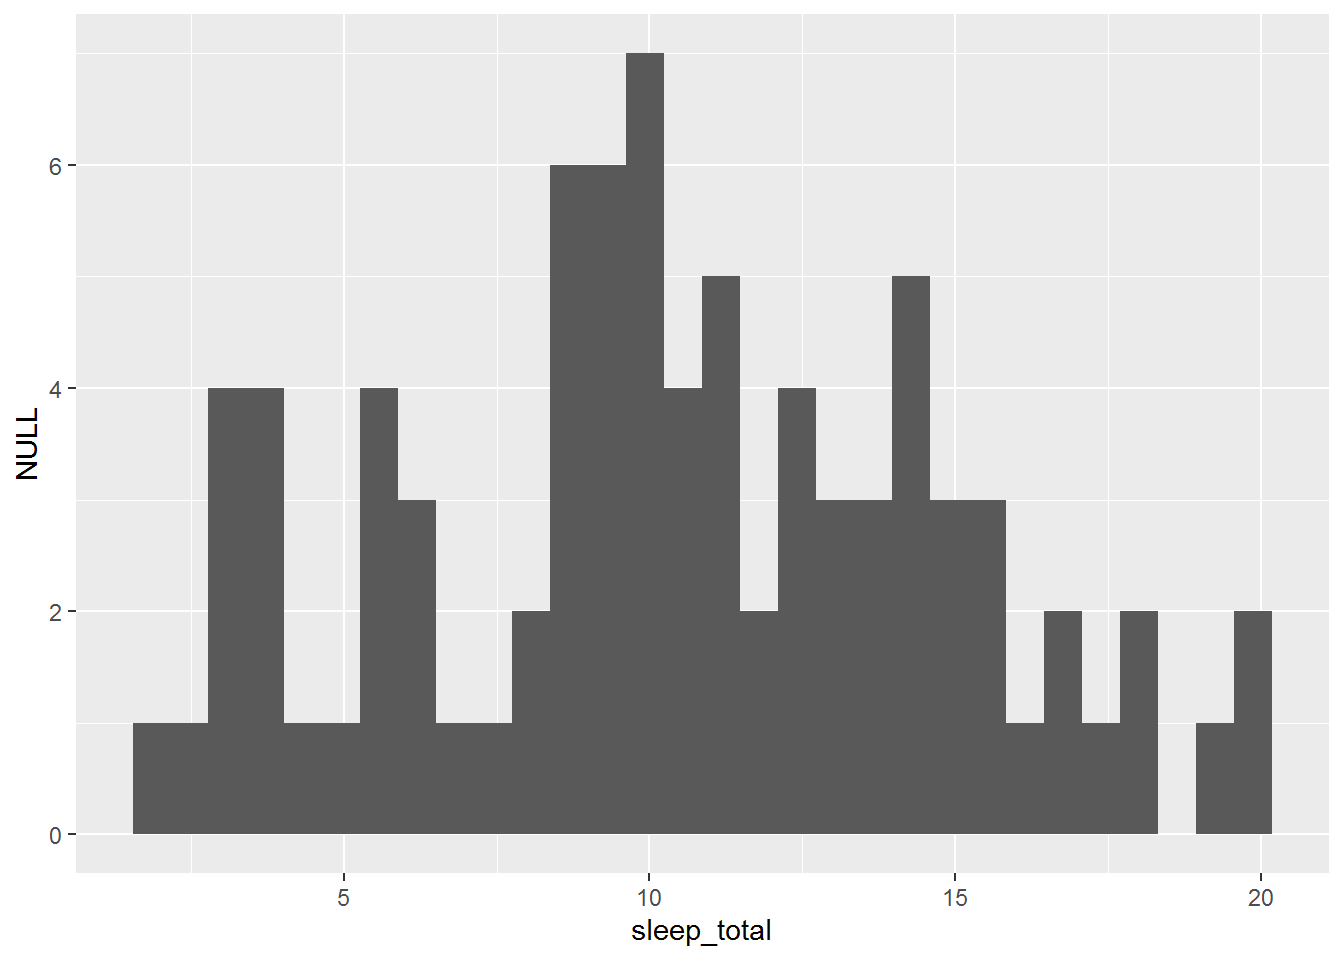
\includegraphics{graficosConR_files/figure-latex/unnamed-chunk-6-1.pdf}

La altura de cada barra en el histograma es proporcional a la frecuencia de datos que caen en el intervalo correspondiente. Por defecto, en la función \texttt{qplot}el número de barras es igual a \texttt{bins=30}. Este valor es muy arbitrario. Otra alternativa consiste en elegir un número \(k\) de barras en función del tamaña muestral \(n\), como por ejemplo, el criterio de Sturges (\(k=1+\log_2(n)\)) o el criterio de Rule (\(k=2n^{1/3}\)). Abajo, un histograma con un número de barras que sigue este ultimo criterio:

\begin{Shaded}
\begin{Highlighting}[]
\FunctionTok{qplot}\NormalTok{(sleep\_total,}\AttributeTok{data=}\NormalTok{msleep,}\AttributeTok{bins=}\DecValTok{8}\NormalTok{,}\AttributeTok{color=}\FunctionTok{I}\NormalTok{(}\StringTok{"grey70"}\NormalTok{),}\AttributeTok{fill=}\FunctionTok{I}\NormalTok{(}\StringTok{"lightblue"}\NormalTok{))}
\end{Highlighting}
\end{Shaded}

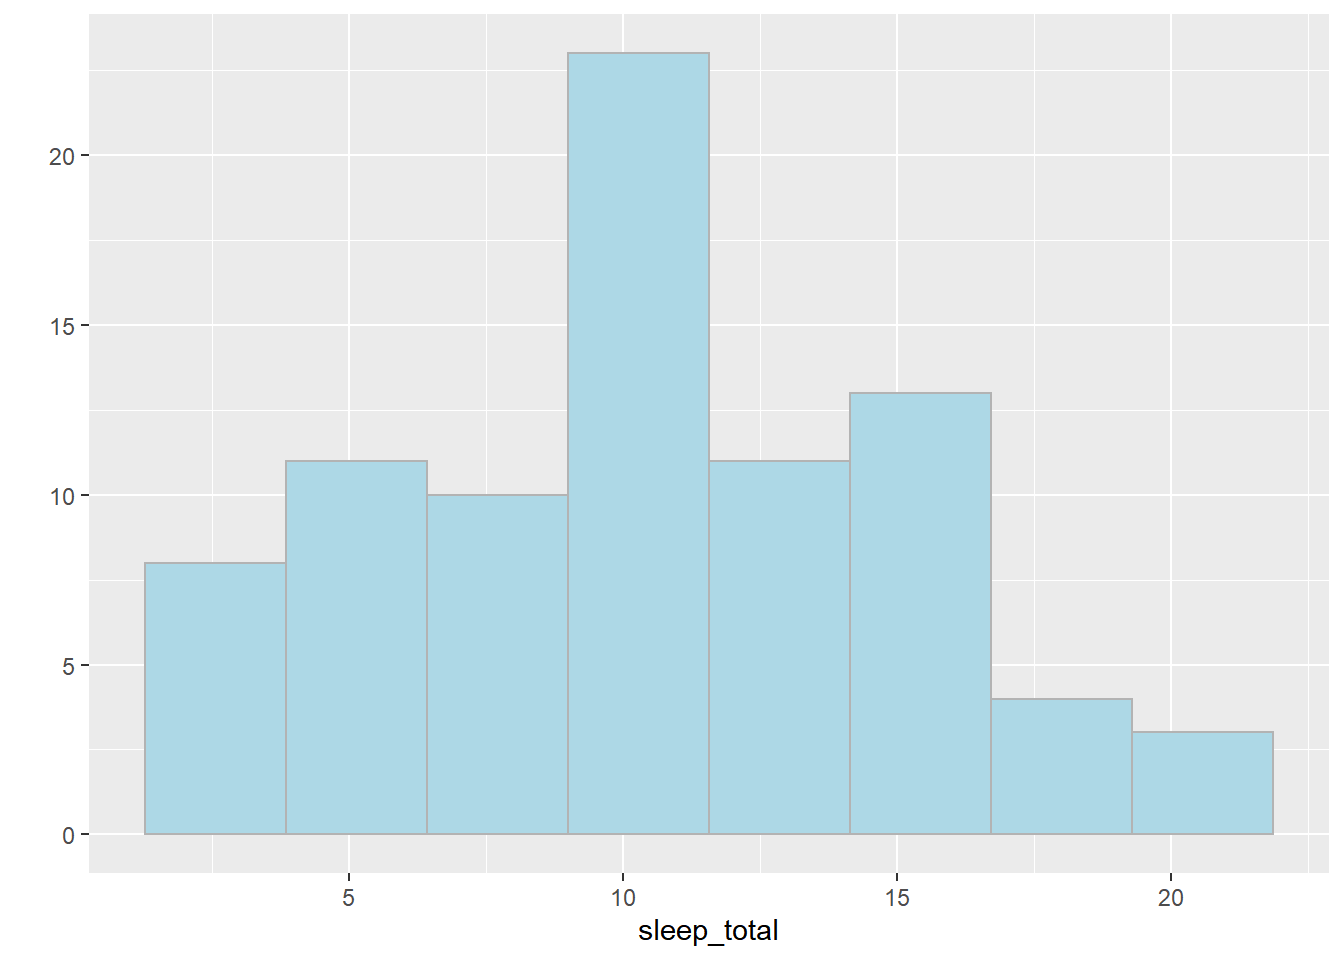
\includegraphics{graficosConR_files/figure-latex/unnamed-chunk-7-1.pdf}

\begin{nota}
El argumento \texttt{fill}controla el color de relleno de las barras y
el argumento \texttt{color} el color del borde. Para especificar un
color concreto se utiliza la función I(). Si el color varía con otra
variable \textbf{z}, se especifica esta dependencia escribiendo
fill=\textbf{z}.
\end{nota}

\begin{Shaded}
\begin{Highlighting}[]
\FunctionTok{qplot}\NormalTok{(sleep\_total,}\AttributeTok{data=}\NormalTok{msleep,}\AttributeTok{bins=}\DecValTok{12}\NormalTok{,}\AttributeTok{fill=}\NormalTok{vore) }\CommentTok{\#distribución del tiempo de sueño según dieta del mamifero. Representación poco adecuada en general.}
\end{Highlighting}
\end{Shaded}

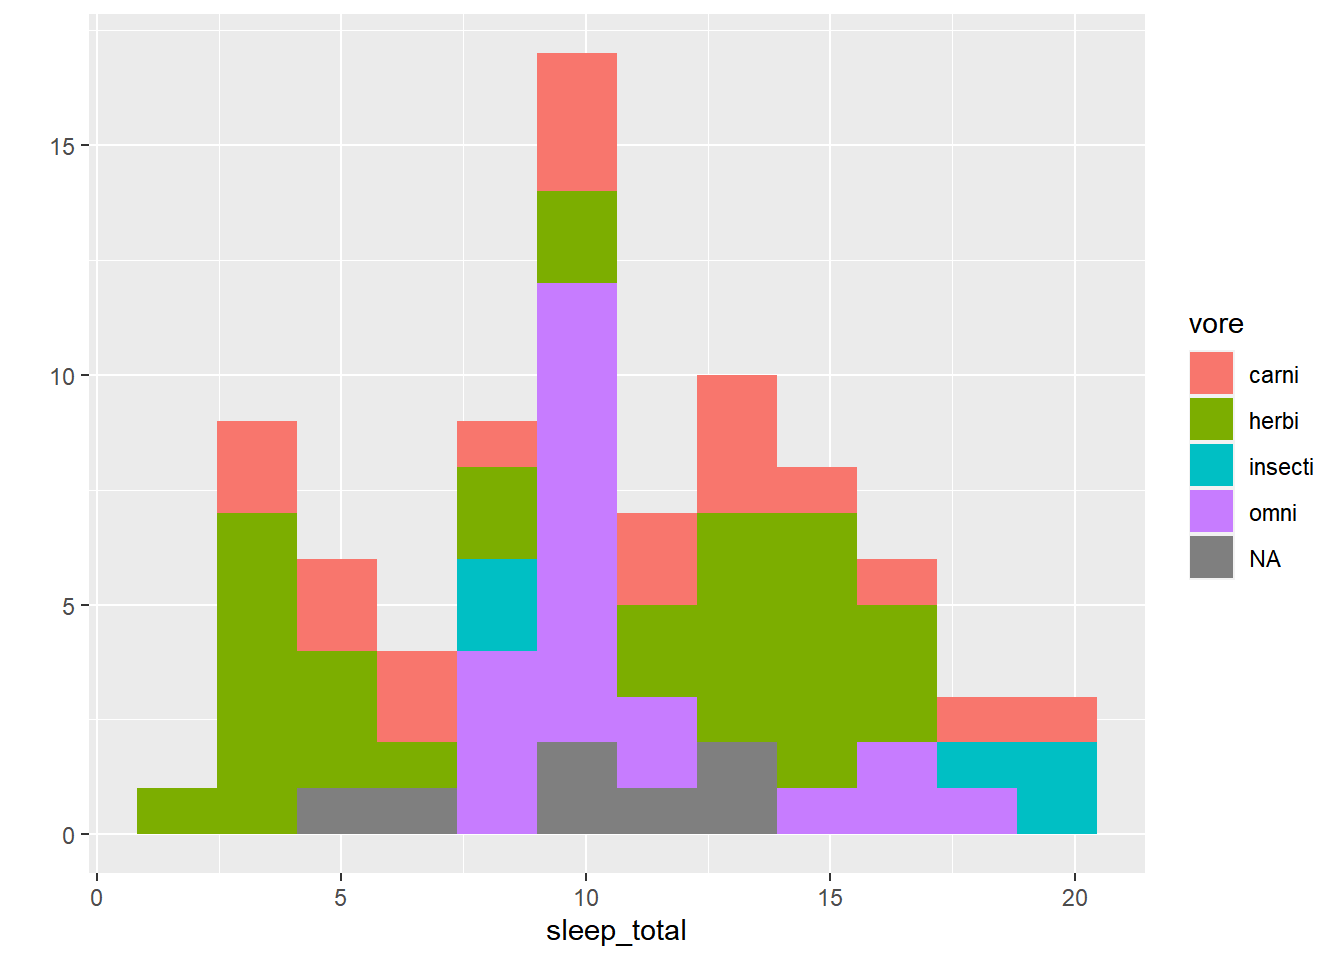
\includegraphics{graficosConR_files/figure-latex/unnamed-chunk-9-1.pdf}

\hypertarget{diagrama-de-caja-boxplot}{%
\subsubsection{Diagrama de caja (boxplot)}\label{diagrama-de-caja-boxplot}}

Otra representación similar es el diagrama de caja. Este diagrama describe la distribución de una variable numérica mediante una caja y unos segmentos que acotan las regiones donde la variable tiene el grueso de sus valores. Esta representación es menos fina que la del histograma pero es más robusta (menos sensible a valores extremos).

Esta representación es especialmente adecuada cuando se quiere describir como varía la distribución de una variable numérica en función de una variable categórica. Así, la distribución del tiempo de sueño según la dieta del mamífero se puede representar de la siguiente manera:

\begin{Shaded}
\begin{Highlighting}[]
\FunctionTok{qplot}\NormalTok{(vore,sleep\_total,}\AttributeTok{data=}\NormalTok{msleep,}\AttributeTok{geom=}\StringTok{"boxplot"}\NormalTok{,}\AttributeTok{xlab=}\StringTok{"Dieta"}\NormalTok{)}
\end{Highlighting}
\end{Shaded}

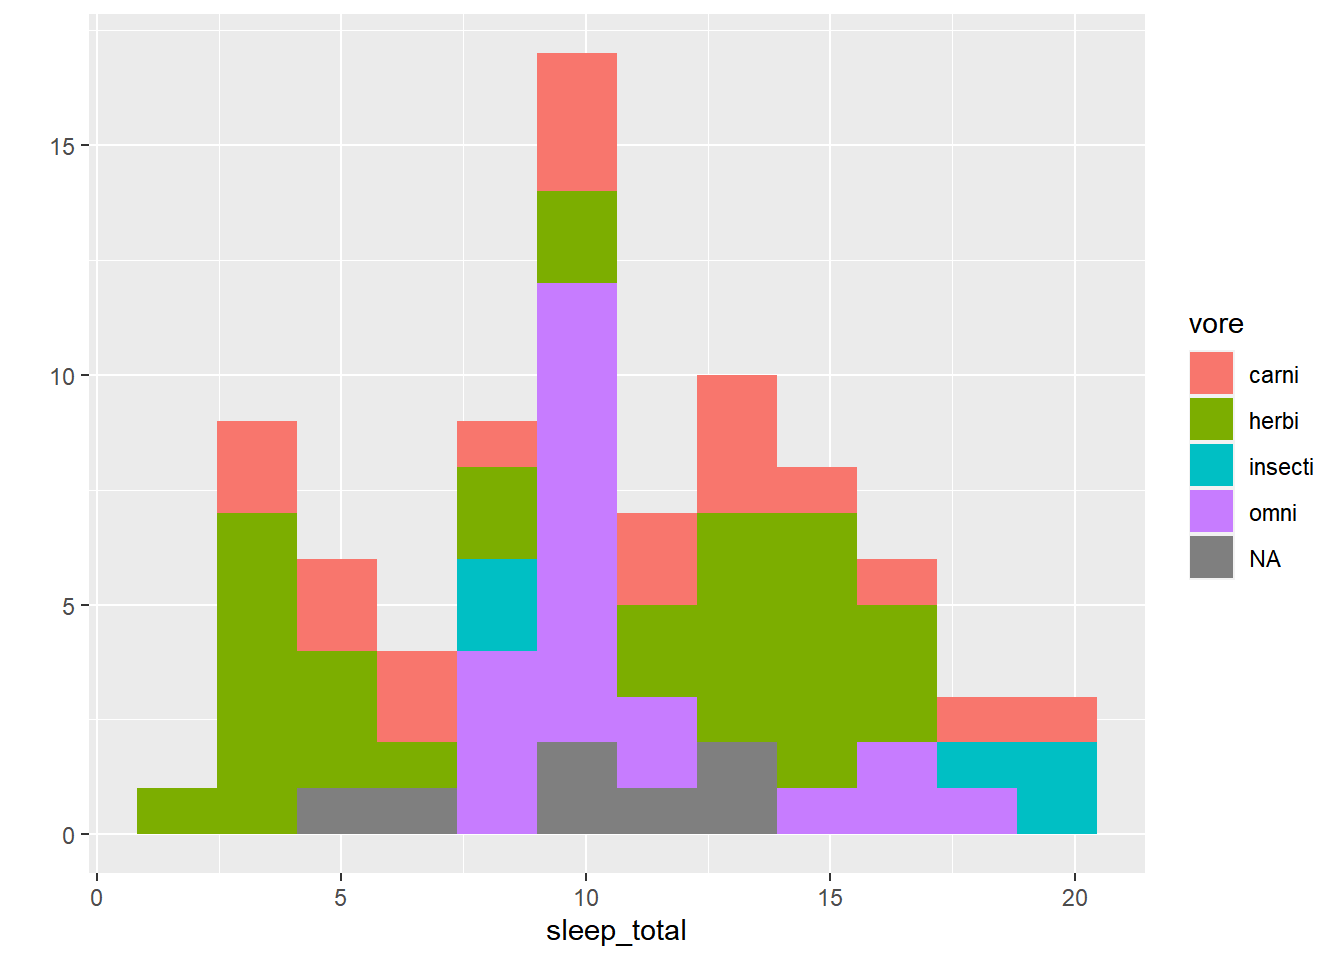
\includegraphics{graficosConR_files/figure-latex/unnamed-chunk-10-1.pdf}

\begin{ej}
Cargar la base de datos de la encuesta nacional americana \texttt{nhs} y
representar la distribución del índice de masa corporal (imc) según el
sexo y la raza.
\end{ej}

\begin{Shaded}
\begin{Highlighting}[]
\FunctionTok{load}\NormalTok{(}\StringTok{"data/nhs.RDA"}\NormalTok{)}
\CommentTok{\#View(nhs)}
\end{Highlighting}
\end{Shaded}

\hypertarget{diagrama-de-barras}{%
\subsubsection{Diagrama de barras}\label{diagrama-de-barras}}

Los diagramas de barras permiten representar la distribución de una variable categórica. En esta representación, cada categoría viene representada por una barra cuya altura es proporcional a su frecuencia en la muestra.

\begin{Shaded}
\begin{Highlighting}[]
\FunctionTok{qplot}\NormalTok{(raza,}\AttributeTok{data=}\NormalTok{nhs) }\CommentTok{\#Distribución de las razas en la muestra de la encuesta americana }
\end{Highlighting}
\end{Shaded}

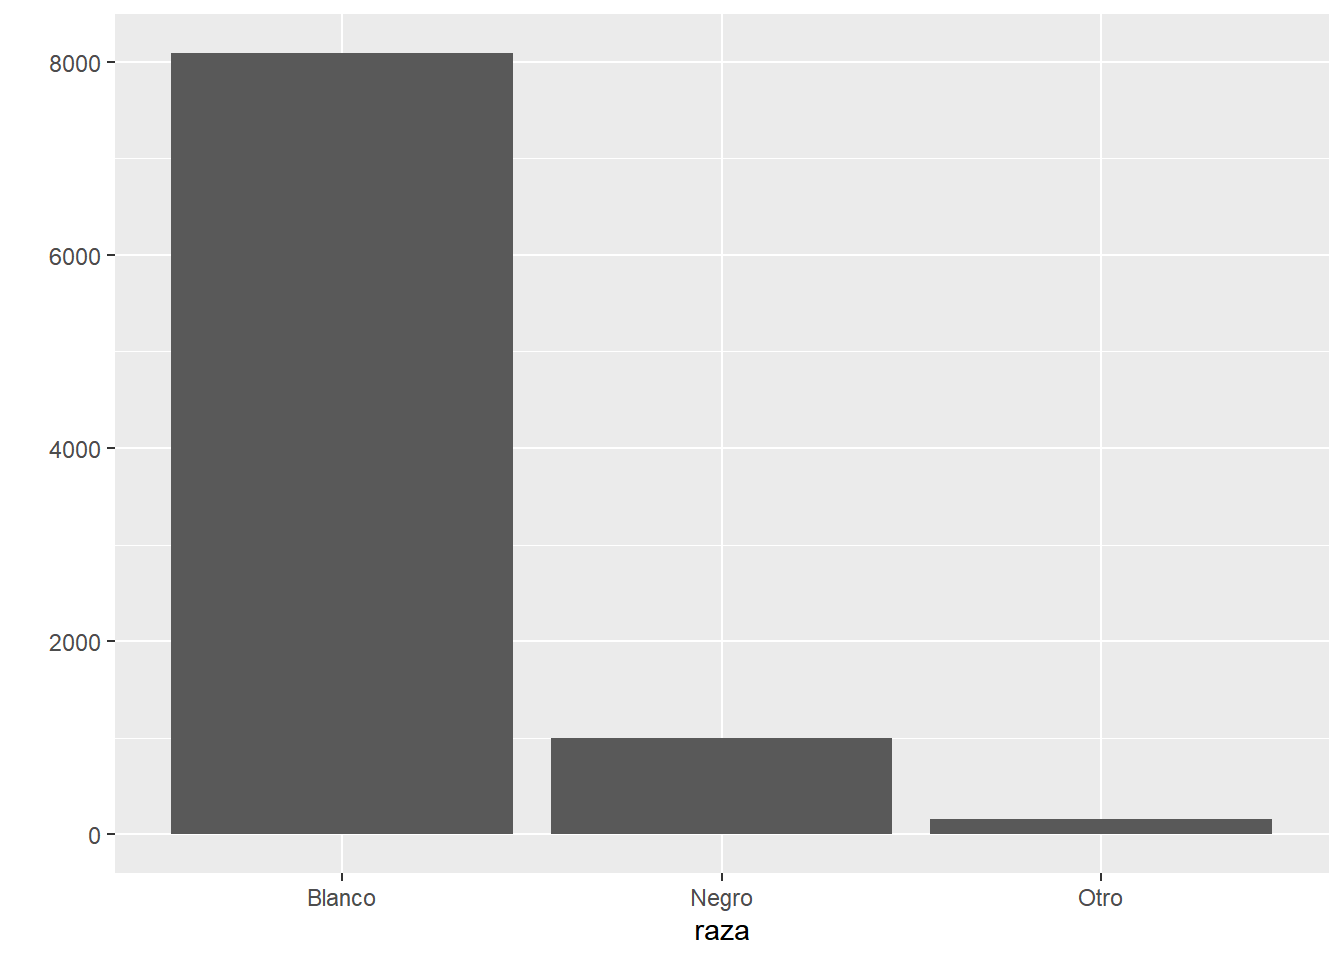
\includegraphics{graficosConR_files/figure-latex/unnamed-chunk-13-1.pdf}

\begin{Shaded}
\begin{Highlighting}[]
\FunctionTok{qplot}\NormalTok{(raza,}\AttributeTok{data=}\NormalTok{nhs,}\AttributeTok{fill=}\NormalTok{sexo,}\AttributeTok{color=}\FunctionTok{I}\NormalTok{(}\StringTok{"black"}\NormalTok{)) }\CommentTok{\#Distribución del sexo segun la raza \textasciigrave{}\textasciigrave{}\textasciigrave{}}
\end{Highlighting}
\end{Shaded}

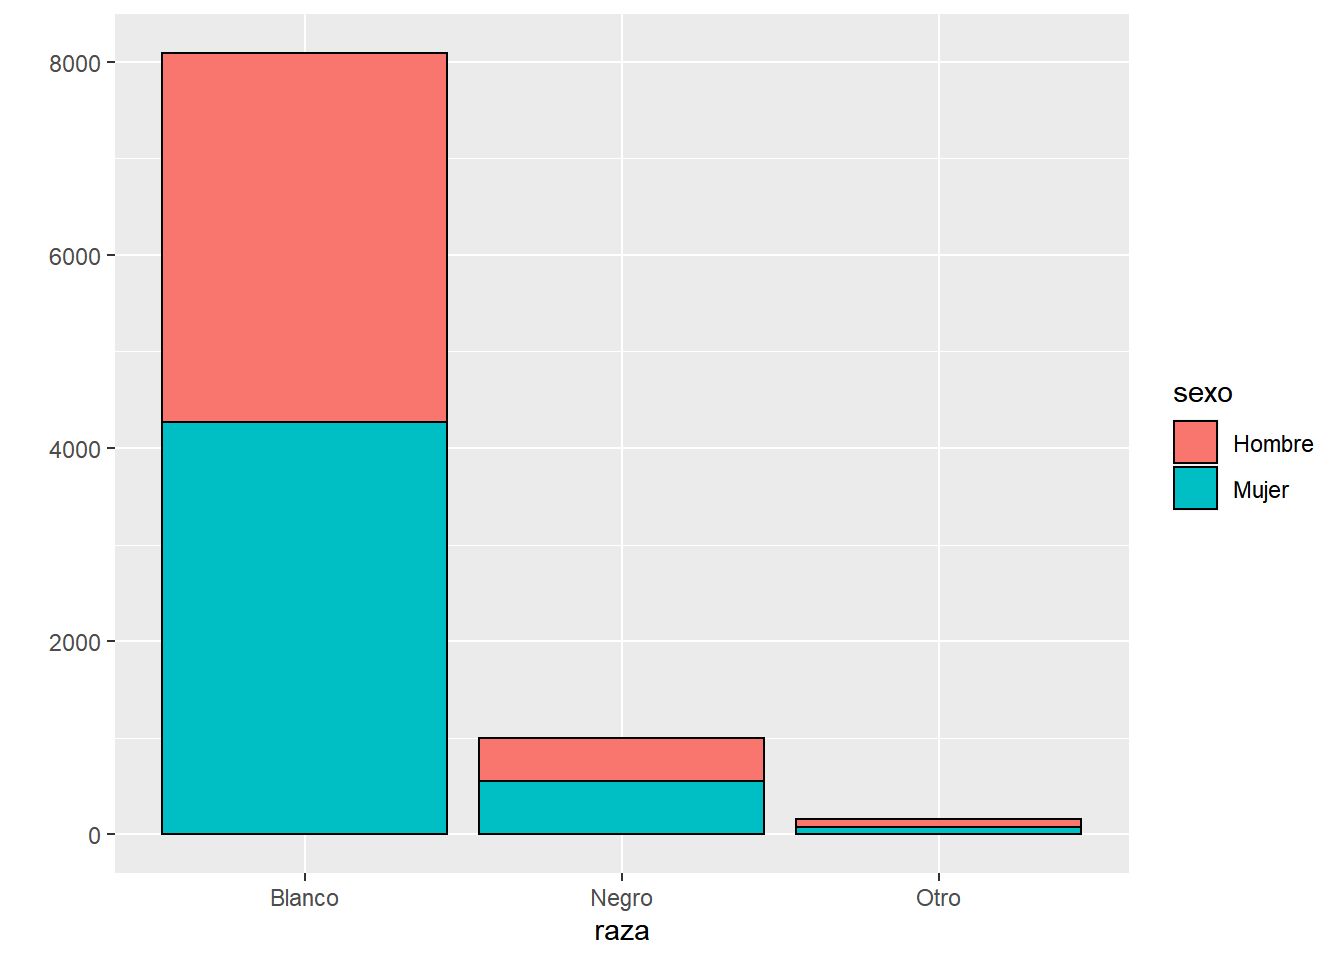
\includegraphics{graficosConR_files/figure-latex/unnamed-chunk-13-2.pdf}

Utilizando el argumento \texttt{fill} se puede ver como varia la distribución de una variable respecto a otra (aquí el sexo según la raza). El gráfico obtenido resulta poco claro y veremos más adelante como mejorarlo.

\begin{ej}
Representar la distribución del ``sobrepeso'' (imc\textgreater25) según
la raza, utilizando la muestra de la encuesta nacional americana.
\end{ej}

\hypertarget{relaciuxf3n-entre-dos-variables}{%
\subsection{Relación entre dos variables}\label{relaciuxf3n-entre-dos-variables}}

\hypertarget{diagrama-de-dispersiuxf3n}{%
\subsubsection{Diagrama de dispersión}\label{diagrama-de-dispersiuxf3n}}

Para describir la relación entre dos variables cuantitativas se suele utilizar gráficos de dispersión. Estos gráficos describen esta relación mediante una nube de puntos en un plano cartesiano. Cada punto de la nube corresponde a una fila de la base de datos y cada una de las variables corresponde a un eje.
En el gráfico siguiente se describe la relación entre las horas de sueño y el peso del animal:

\begin{Shaded}
\begin{Highlighting}[]
\FunctionTok{qplot}\NormalTok{(bodywt,sleep\_total,}\AttributeTok{data=}\NormalTok{msleep,}\AttributeTok{xlab=}\StringTok{"peso (en kg, escala log)"}\NormalTok{,}\AttributeTok{log=}\StringTok{"x"}\NormalTok{)}
\end{Highlighting}
\end{Shaded}

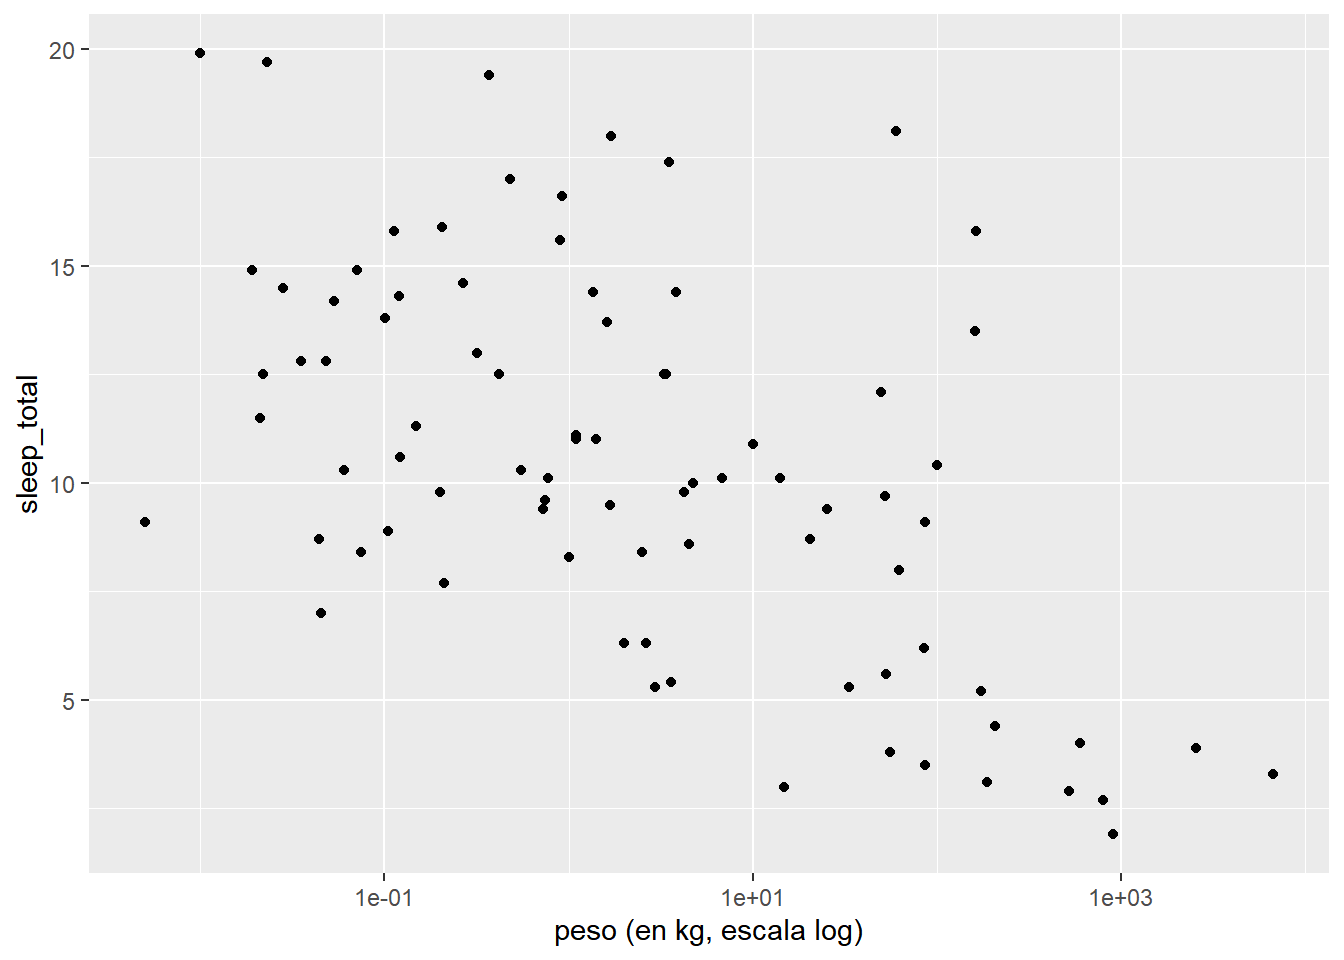
\includegraphics{graficosConR_files/figure-latex/unnamed-chunk-15-1.pdf}

Ajustando una curva suave (``smooth'') a la nube de puntos, se puede apreciar mejor la tendencia en esta relación:

\begin{Shaded}
\begin{Highlighting}[]
\FunctionTok{qplot}\NormalTok{(bodywt,sleep\_total,}\AttributeTok{data=}\NormalTok{msleep,}\AttributeTok{log=}\StringTok{"x"}\NormalTok{,}\AttributeTok{geom=}\StringTok{"smooth"}\NormalTok{)}
\end{Highlighting}
\end{Shaded}

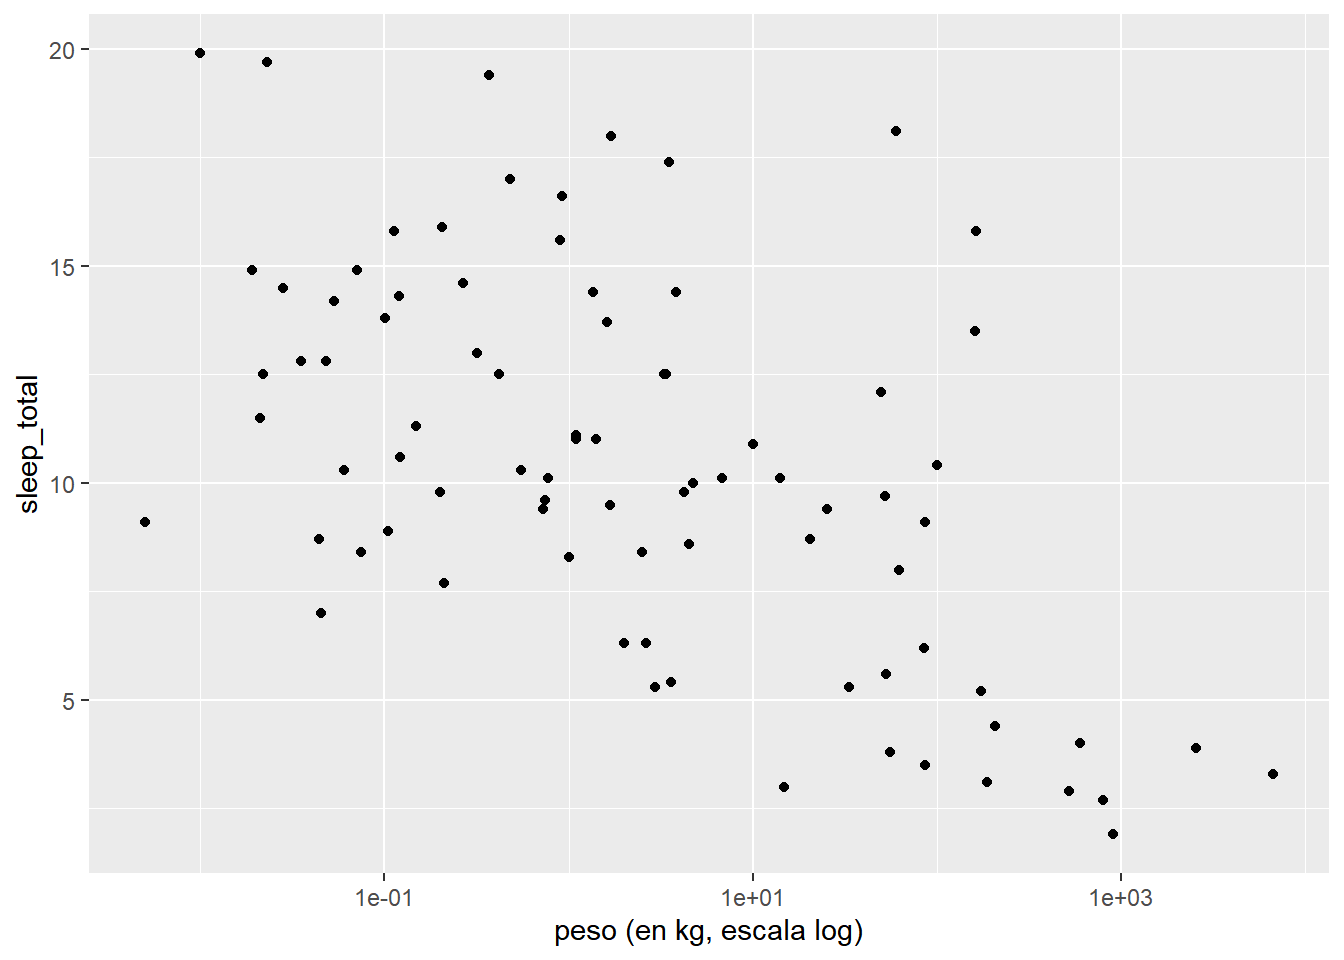
\includegraphics{graficosConR_files/figure-latex/unnamed-chunk-16-1.pdf}

\begin{Shaded}
\begin{Highlighting}[]
\CommentTok{\#qplot(bodywt,sleep\_total,data=msleep,log="x",geom="smooth", method="lm") \#\# para ajutar una recta; "lm": linear model}
\end{Highlighting}
\end{Shaded}

Para evitar los problemas de solapamiento de puntos en la representación se puede poner algo de ruido en los datos ( \texttt{geom="jitter"} ), jugar con el tamaño de los puntos (\texttt{size}) o utilizar el parámetro de transparencia (\texttt{alpha}):

\begin{Shaded}
\begin{Highlighting}[]
\FunctionTok{qplot}\NormalTok{(edad, imc,}\AttributeTok{data=}\NormalTok{nhs,}\AttributeTok{alpha=}\FunctionTok{I}\NormalTok{(.}\DecValTok{1}\NormalTok{),}\AttributeTok{size=}\FunctionTok{I}\NormalTok{(}\DecValTok{1}\NormalTok{))}
\end{Highlighting}
\end{Shaded}

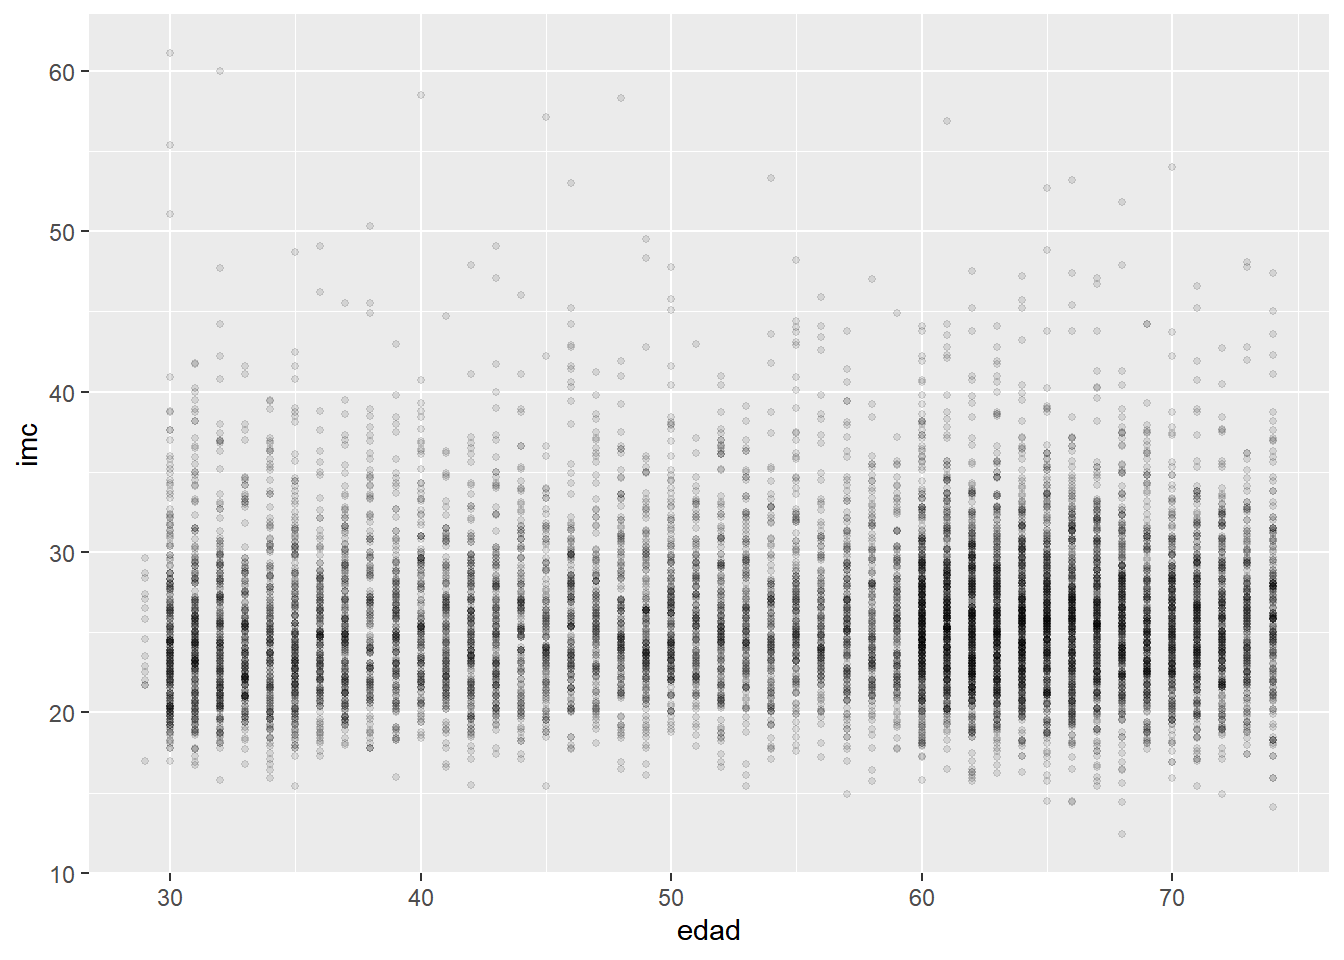
\includegraphics{graficosConR_files/figure-latex/unnamed-chunk-17-1.pdf}

\begin{Shaded}
\begin{Highlighting}[]
\CommentTok{\#qplot(edad, imc,data=nhs, alpha=I(.1),size=I(1), geom="jitter") \#Mejor resultado añadiendo algo de ruido}
\end{Highlighting}
\end{Shaded}

\begin{ej}
Utilizando la encuesta nacional americana, describir la relación entre
la edad y la presión arterial sistólica. En un mismo gráfico, describir
como esta relación cambia con el sexo.
\end{ej}

\hypertarget{dotchart}{%
\subsubsection{Dotchart}\label{dotchart}}

Si una de las variables es categórica y tiene muchas categorías, el gráfico de dispersión puede ser también apropiado:

\begin{Shaded}
\begin{Highlighting}[]
\FunctionTok{qplot}\NormalTok{(sleep\_total,order,}\AttributeTok{data=}\NormalTok{msleep,}\AttributeTok{col=}\NormalTok{vore) }
\end{Highlighting}
\end{Shaded}

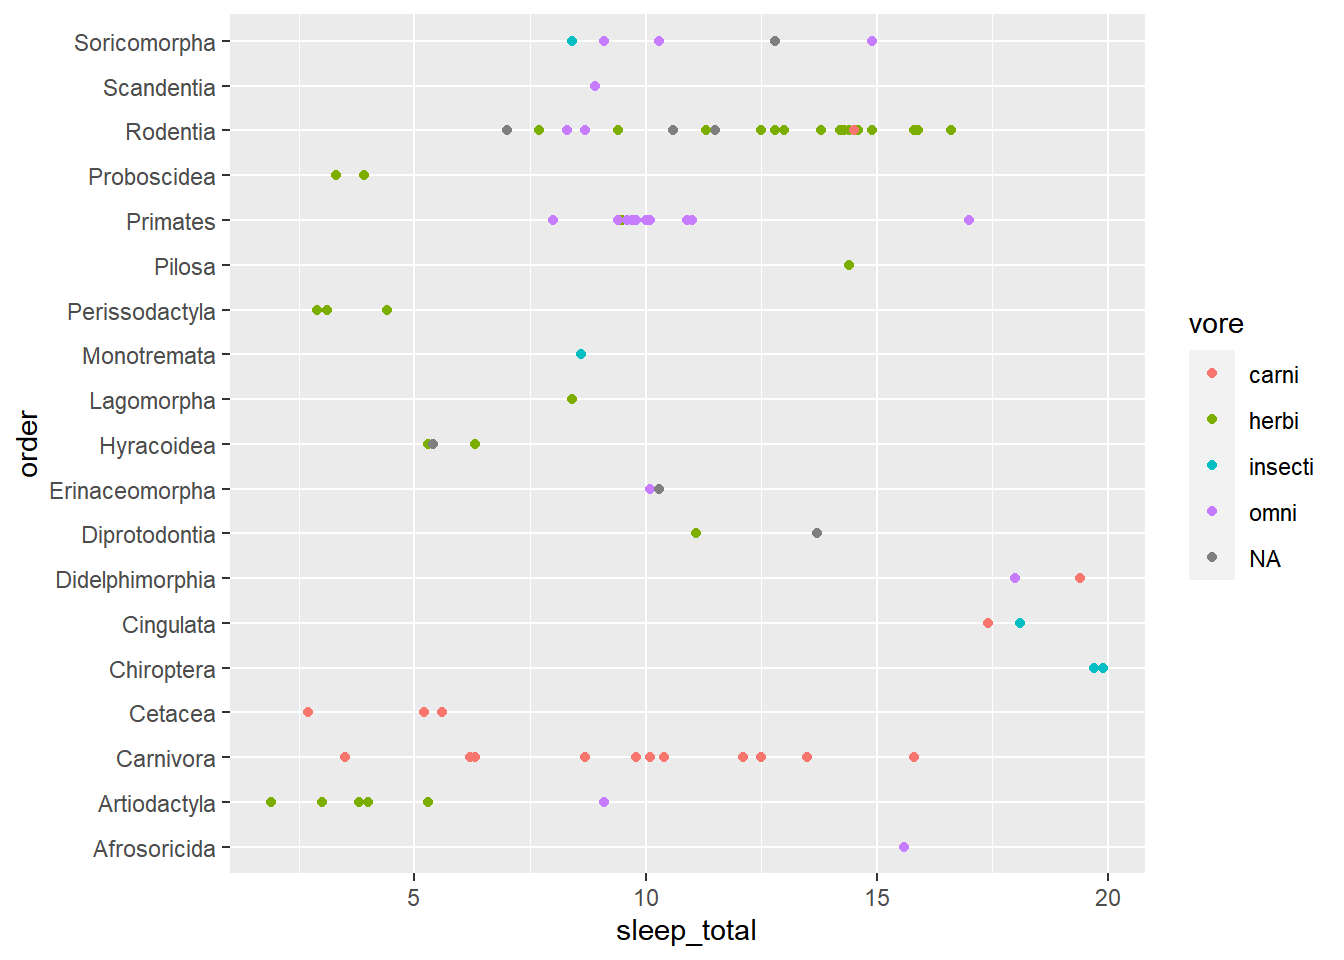
\includegraphics{graficosConR_files/figure-latex/unnamed-chunk-19-1.pdf}

Pero, es recomendable para mayor claridad ordenar la variable categórica de acuerdo a la otra variable:

\begin{Shaded}
\begin{Highlighting}[]
\FunctionTok{qplot}\NormalTok{(sleep\_total,}\FunctionTok{reorder}\NormalTok{(order,sleep\_total),}\AttributeTok{data=}\NormalTok{msleep,}\AttributeTok{col=}\NormalTok{vore,}\AttributeTok{ylab=}\StringTok{"horas de sueño"}\NormalTok{)}
\end{Highlighting}
\end{Shaded}

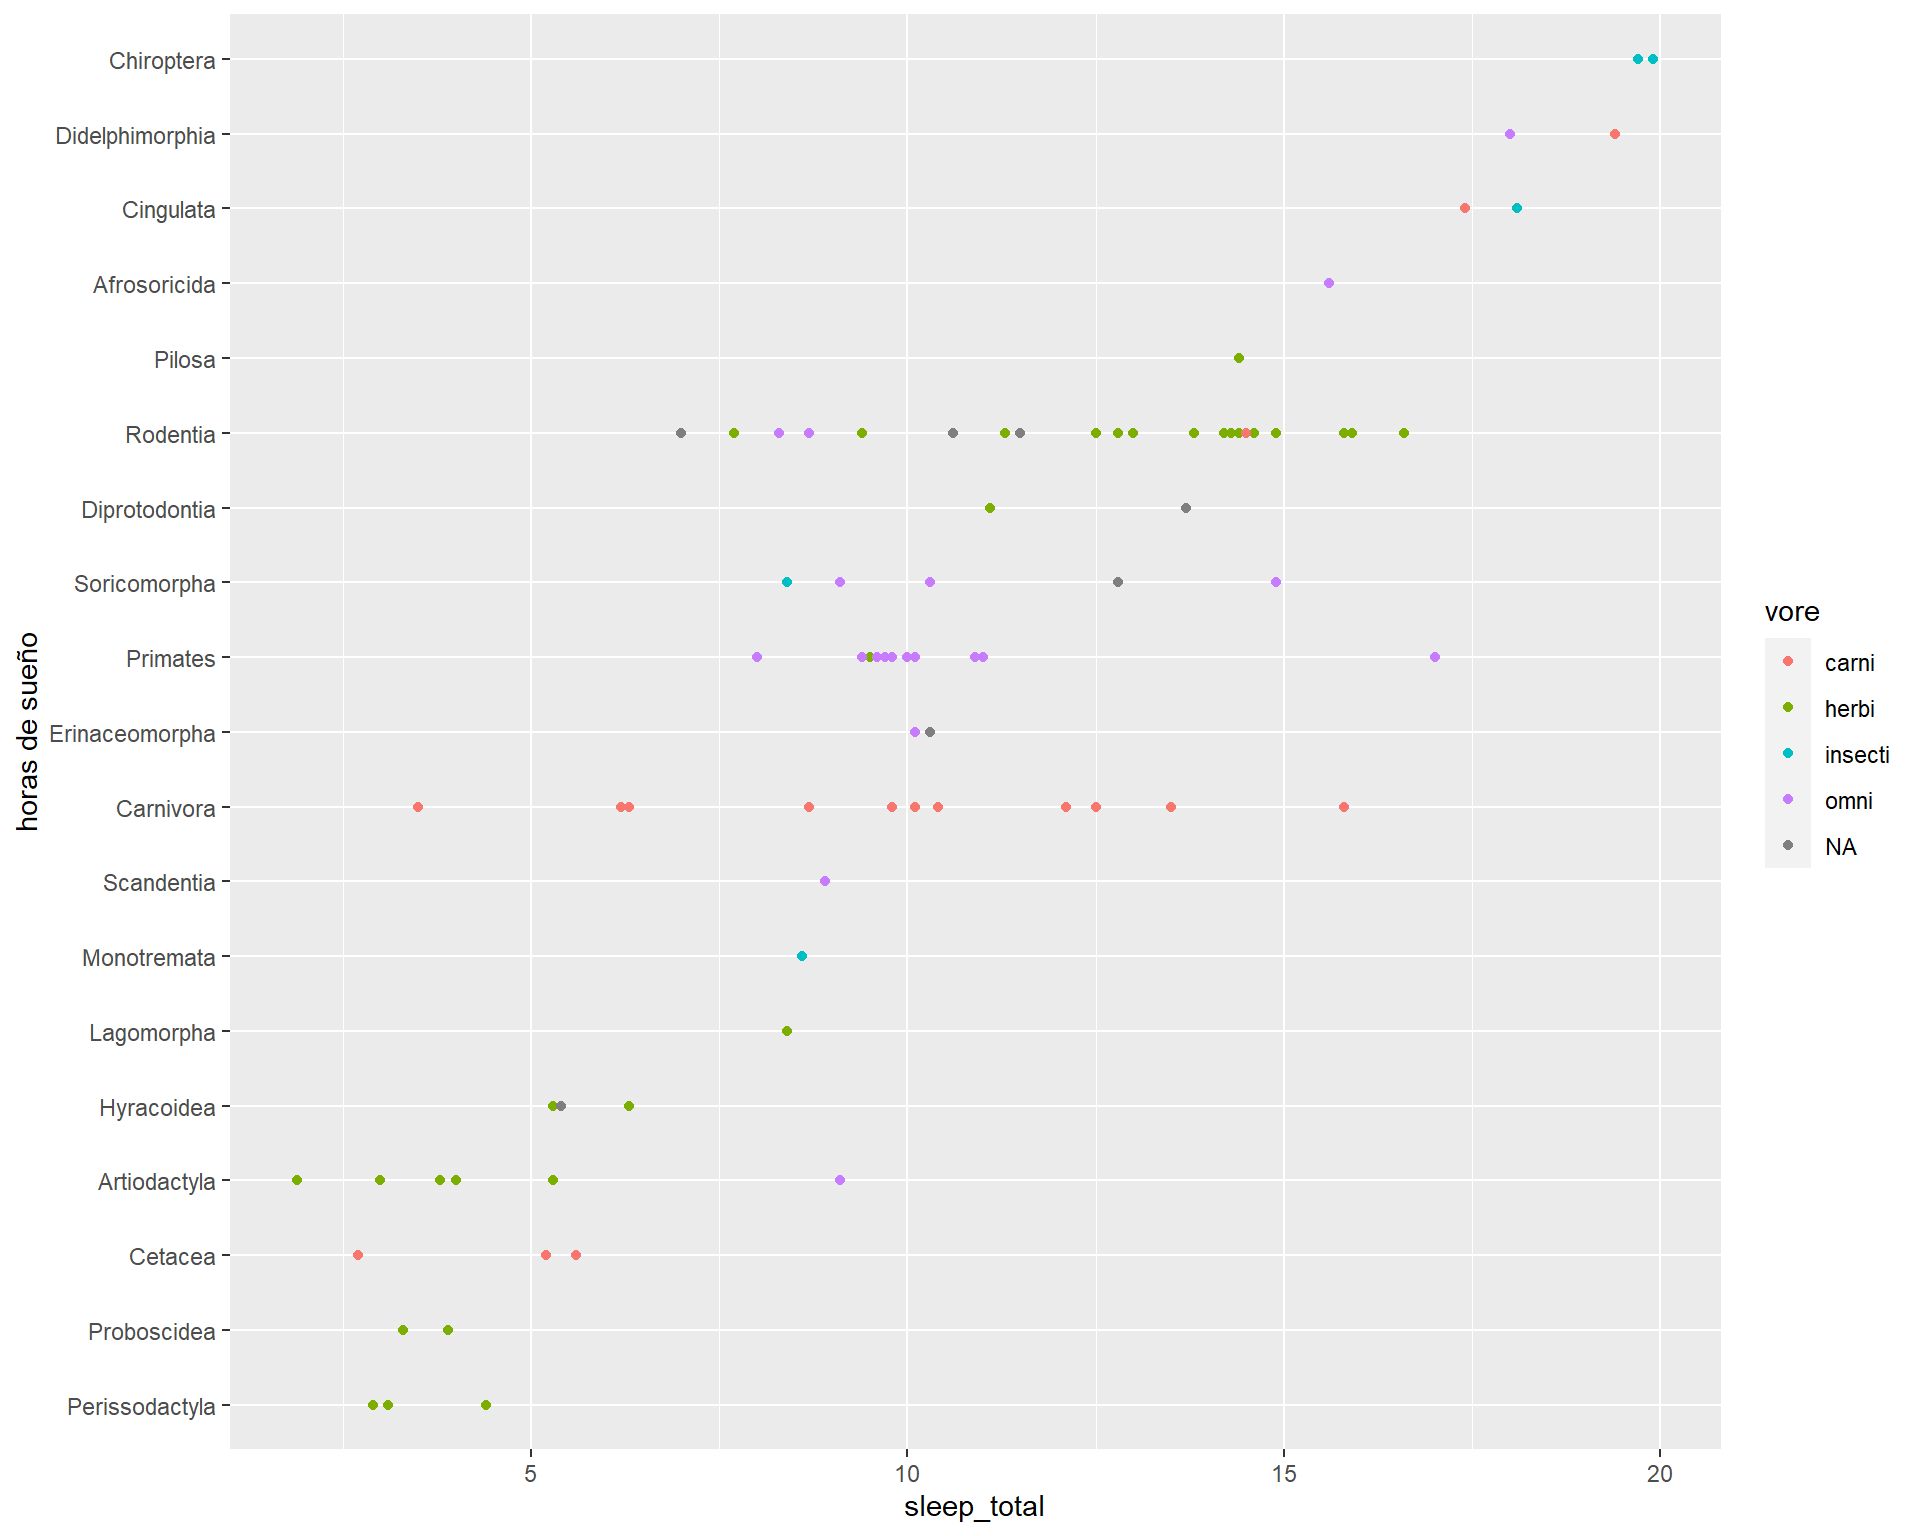
\includegraphics{graficosConR_files/figure-latex/unnamed-chunk-20-1.pdf}

\begin{ej}
Describir con un gráfico similar al anterior, los datos de la base de
datos \texttt{islands} sobre superficies de islas. Puede ser oportuno
recurrir a una escala log.
\end{ej}

\hypertarget{relaciuxf3n-con-una-variable-temporal}{%
\subsubsection{Relación con una variable temporal}\label{relaciuxf3n-con-una-variable-temporal}}

Si una de las variables es el tiempo, a menudo es conveniente recurrir a lineas (\texttt{geom="line"}) en vez de puntos para representar la evolución de la otra variable.

\begin{Shaded}
\begin{Highlighting}[]
\FunctionTok{require}\NormalTok{(gapminder) }\CommentTok{\#base de datos sobre esperanza de vida según caracteristicas socio{-}demograficas del pais}
\NormalTok{datos}\OtherTok{=}\FunctionTok{subset}\NormalTok{(gapminder,country }\SpecialCharTok{\%in\%} \FunctionTok{c}\NormalTok{(}\StringTok{"Spain"}\NormalTok{,}\StringTok{"Greece"}\NormalTok{,}\StringTok{"Poland"}\NormalTok{)) }\CommentTok{\#sólo se consideran España, Grecia y Polonia}
\FunctionTok{qplot}\NormalTok{(year,lifeExp,}\AttributeTok{data=}\NormalTok{datos,}\AttributeTok{geom=}\StringTok{"line"}\NormalTok{,}\AttributeTok{color=}\NormalTok{country)}
\end{Highlighting}
\end{Shaded}

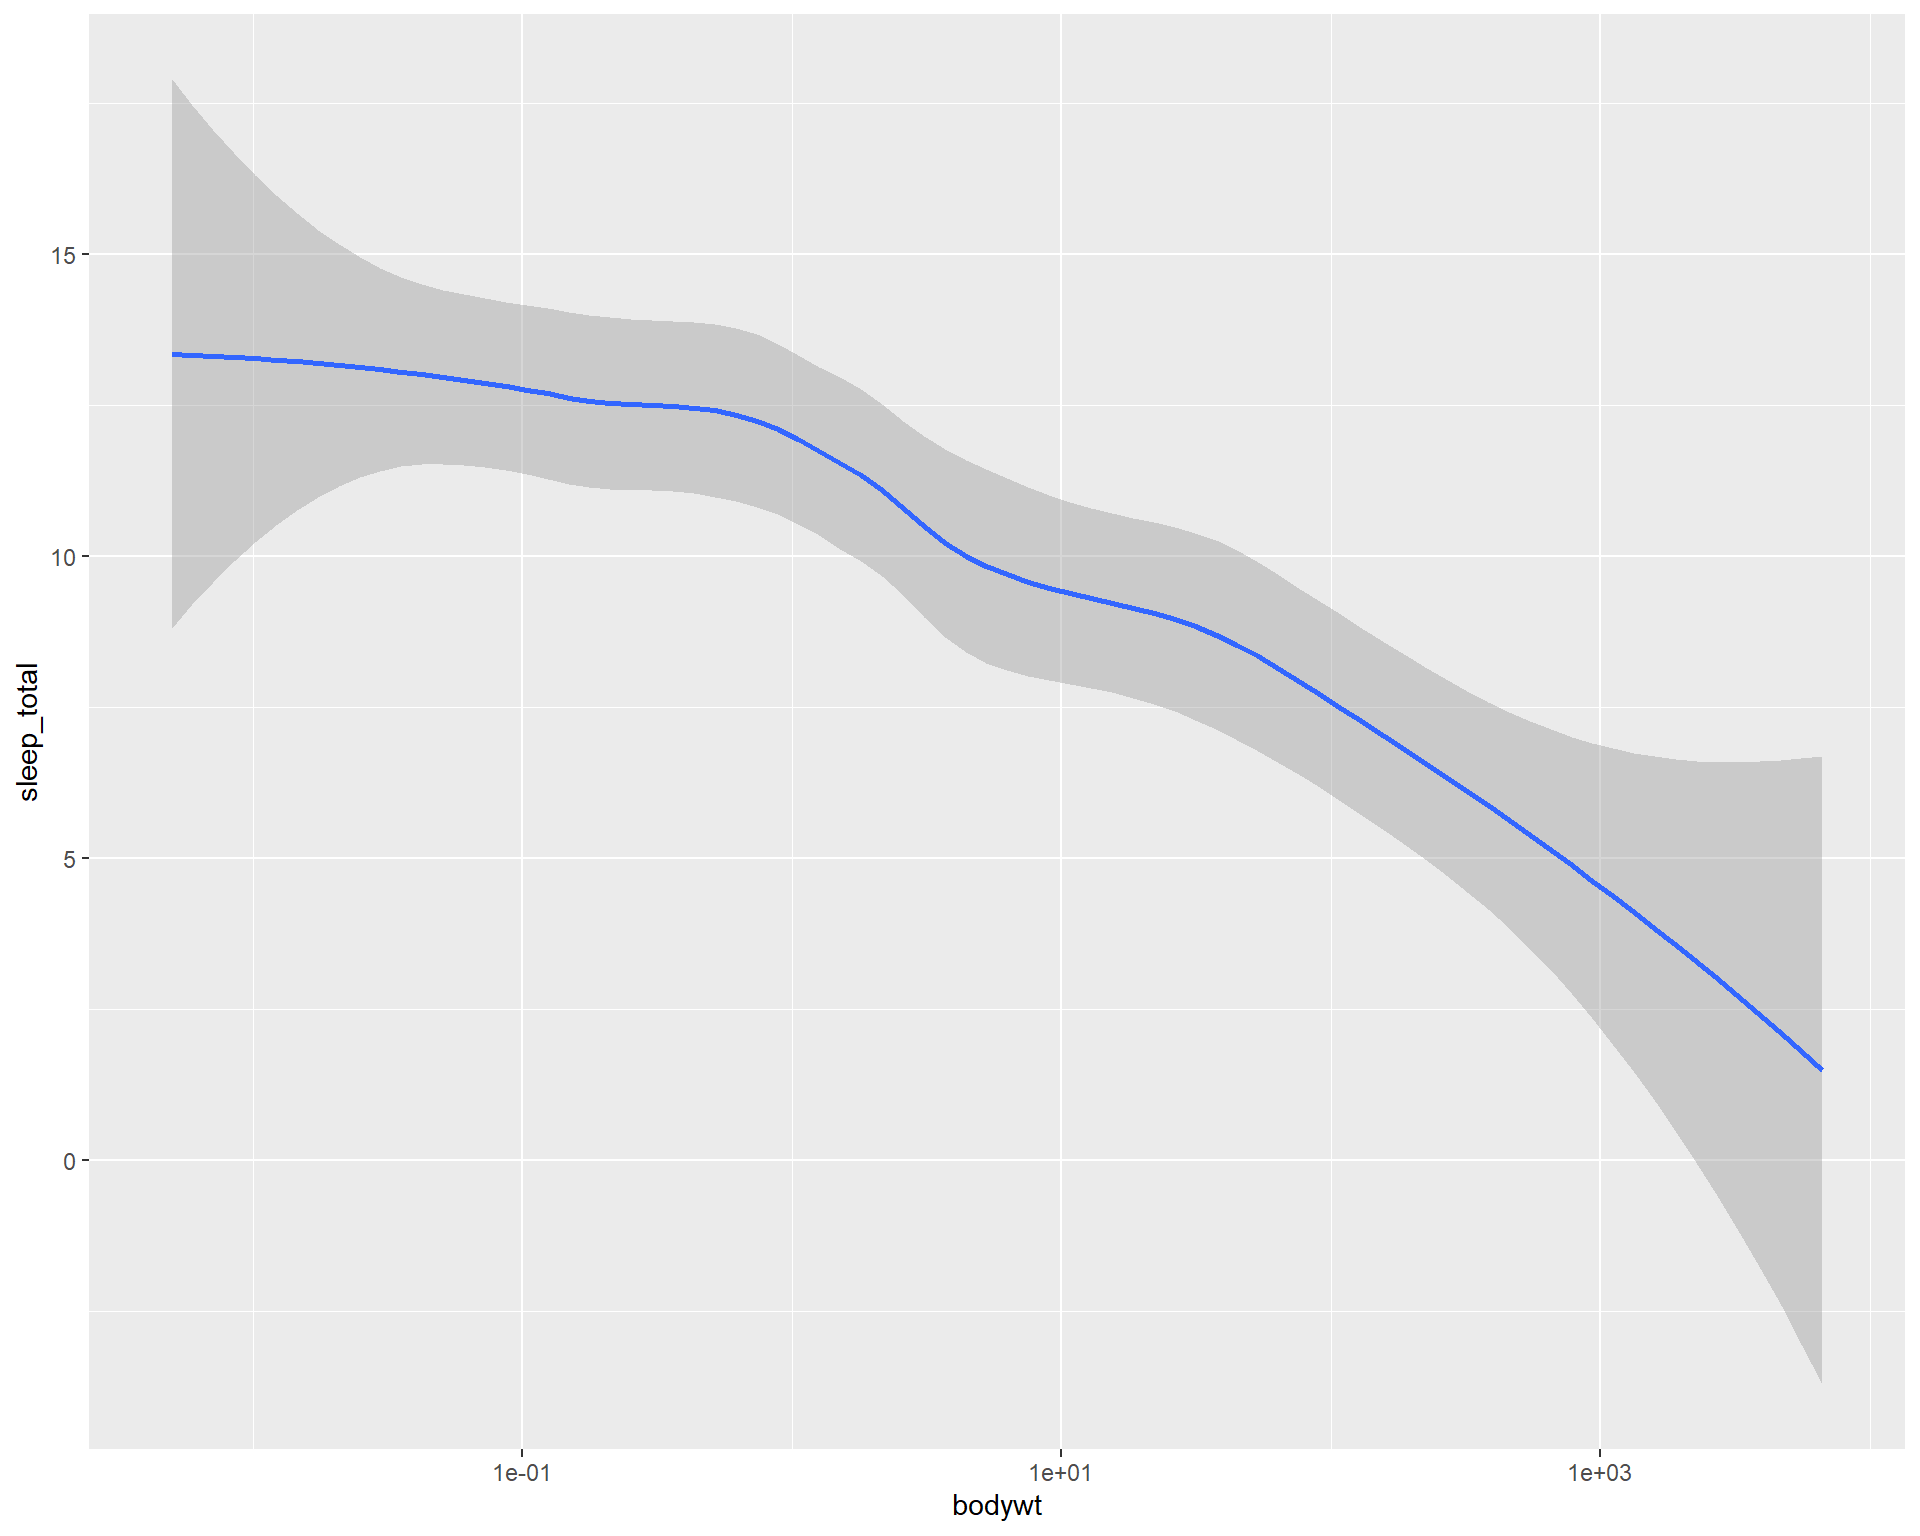
\includegraphics{graficosConR_files/figure-latex/unnamed-chunk-22-1.pdf}

Sin embargo para representar la tendencia en una nube de puntos se utilizará la opción \texttt{geom="smooth"}:

\begin{Shaded}
\begin{Highlighting}[]
\FunctionTok{qplot}\NormalTok{(year,lifeExp,}\AttributeTok{data=}\NormalTok{gapminder,}\AttributeTok{geom=}\StringTok{"smooth"}\NormalTok{,}\AttributeTok{color=}\NormalTok{continent,}\AttributeTok{se=}\ConstantTok{FALSE}\NormalTok{) }\CommentTok{\#se=FALSE para quitar intervalos de confianza}
\end{Highlighting}
\end{Shaded}

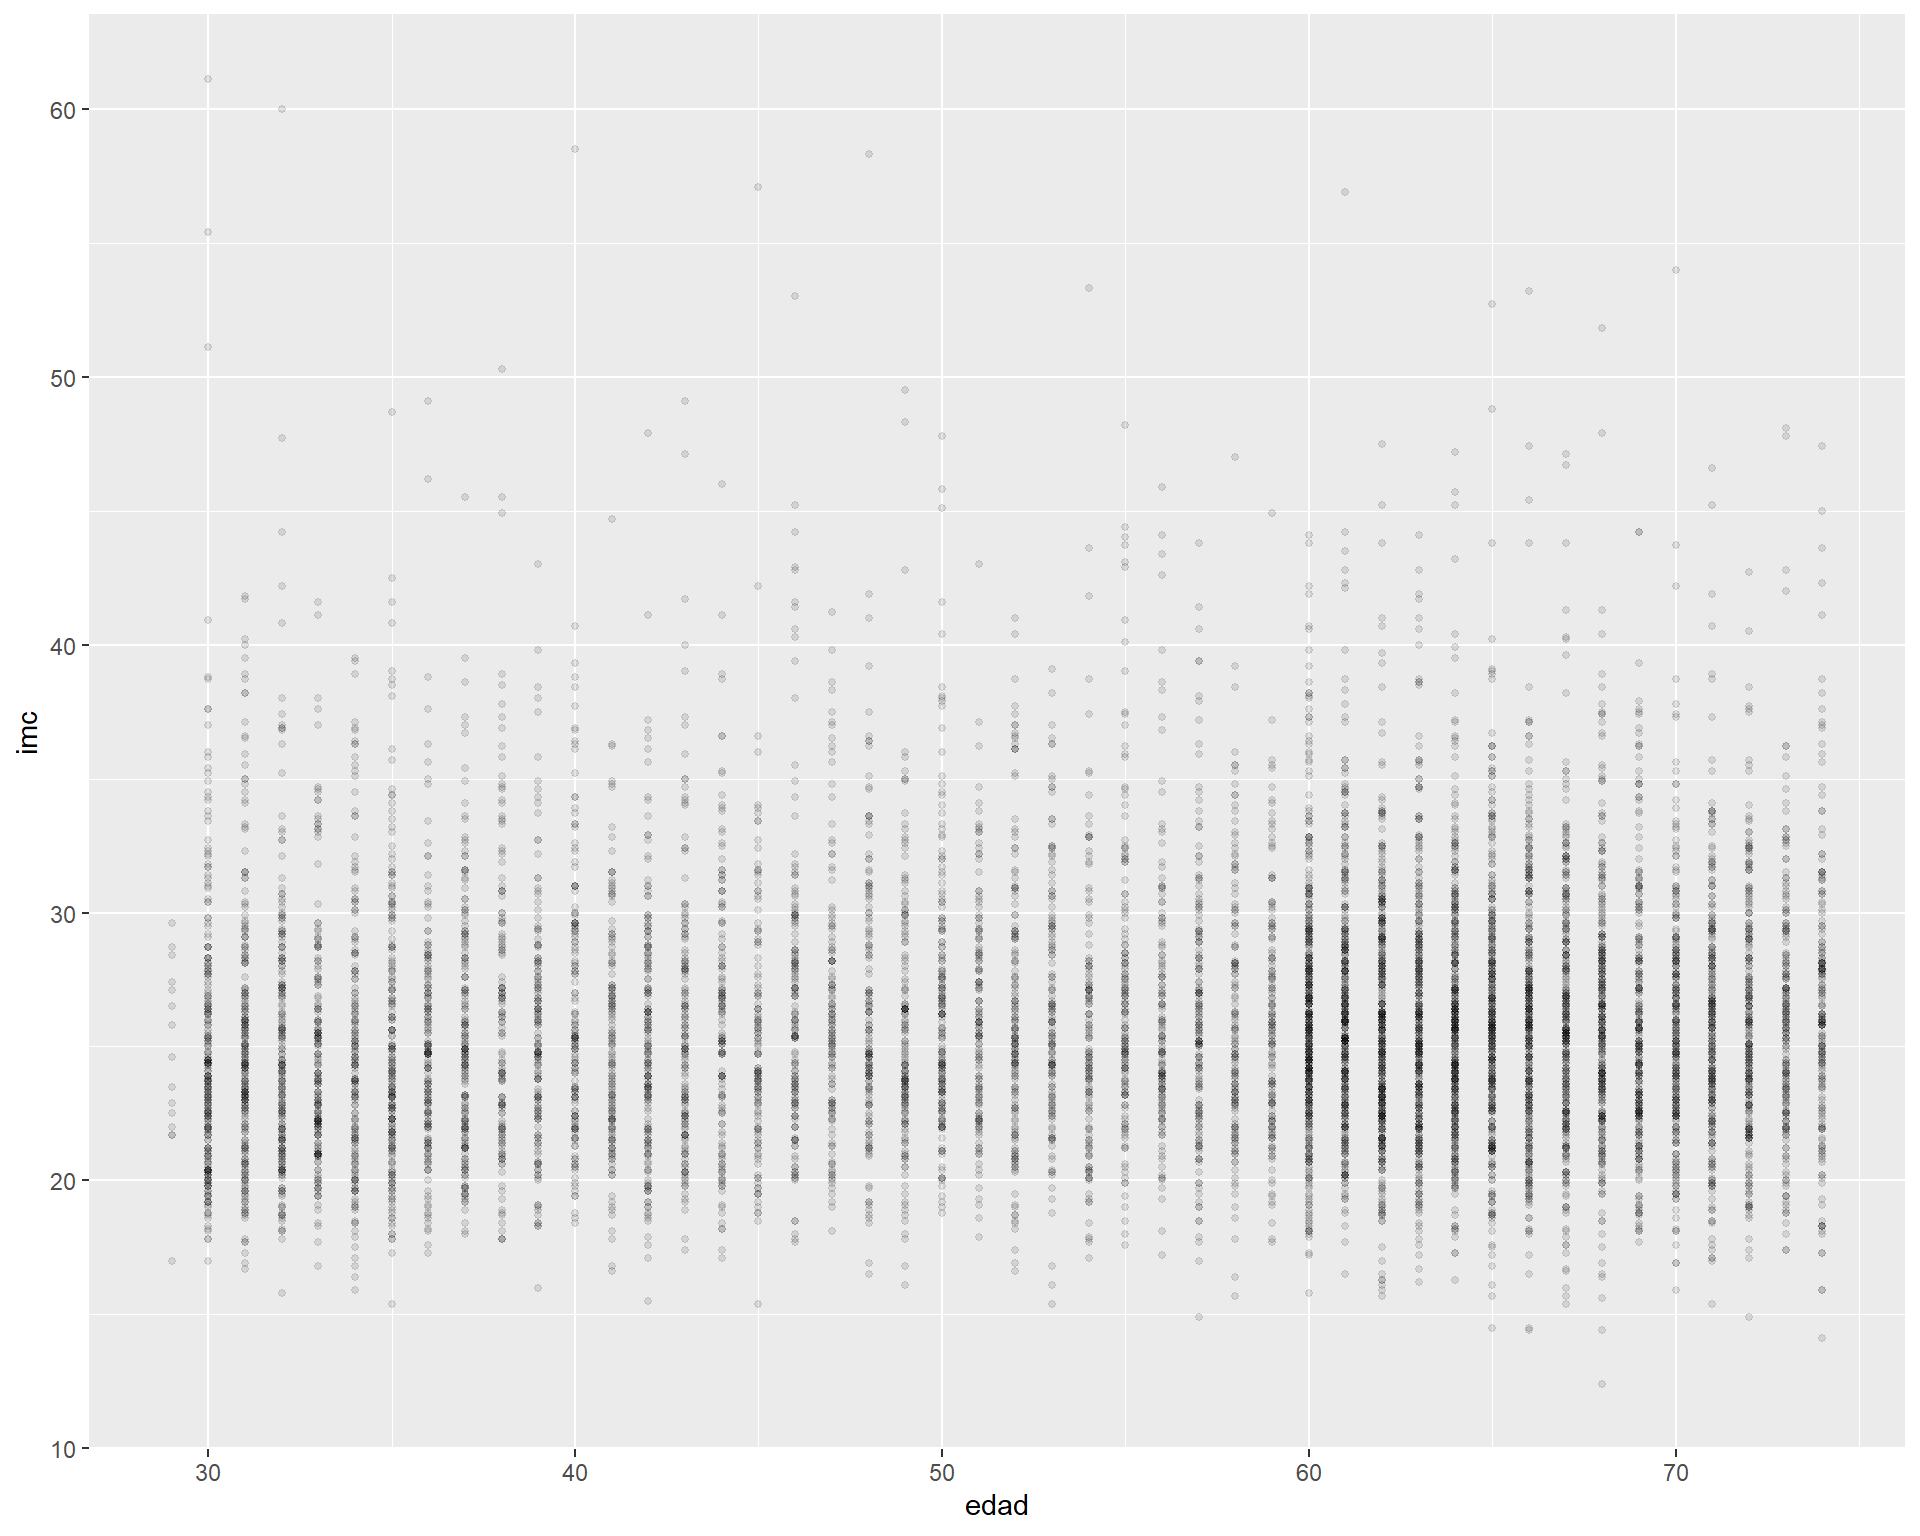
\includegraphics{graficosConR_files/figure-latex/unnamed-chunk-23-1.pdf}

\begin{ej}
Describir con gráficos similares a los anteriores, los datos de la base
de datos \texttt{cancer} sobre la evolución de las tasas de mortalidad
por cáncer en España en el periodo 1975-2012. Empezar por ejemplo,
representando la evolución de la mortalidad por cáncer de pulmón según
el sexo.
\end{ej}

\hypertarget{gruxe1ficos-avanzados}{%
\section{Gráficos avanzados}\label{gruxe1ficos-avanzados}}

Esta sección es una introducción a las ideas del libro \emph{The Grammar of Graphics} de Leland Wilkinson (2005) tal y como vienen implementadas en el paquete \texttt{ggplot2} de Hadley Wickham (2009).

A continuación veremos los elementos principales de esta gramática y como nos permiten elaborar de manera sencilla representaciones visuales del comportamiento de una variable de interés a través de los distintos niveles de otras.

El gráfico siguiente muestra la evolución de la tasa de mortalidad por cáncer según la localización, en España durante el periodo 1975-2012.

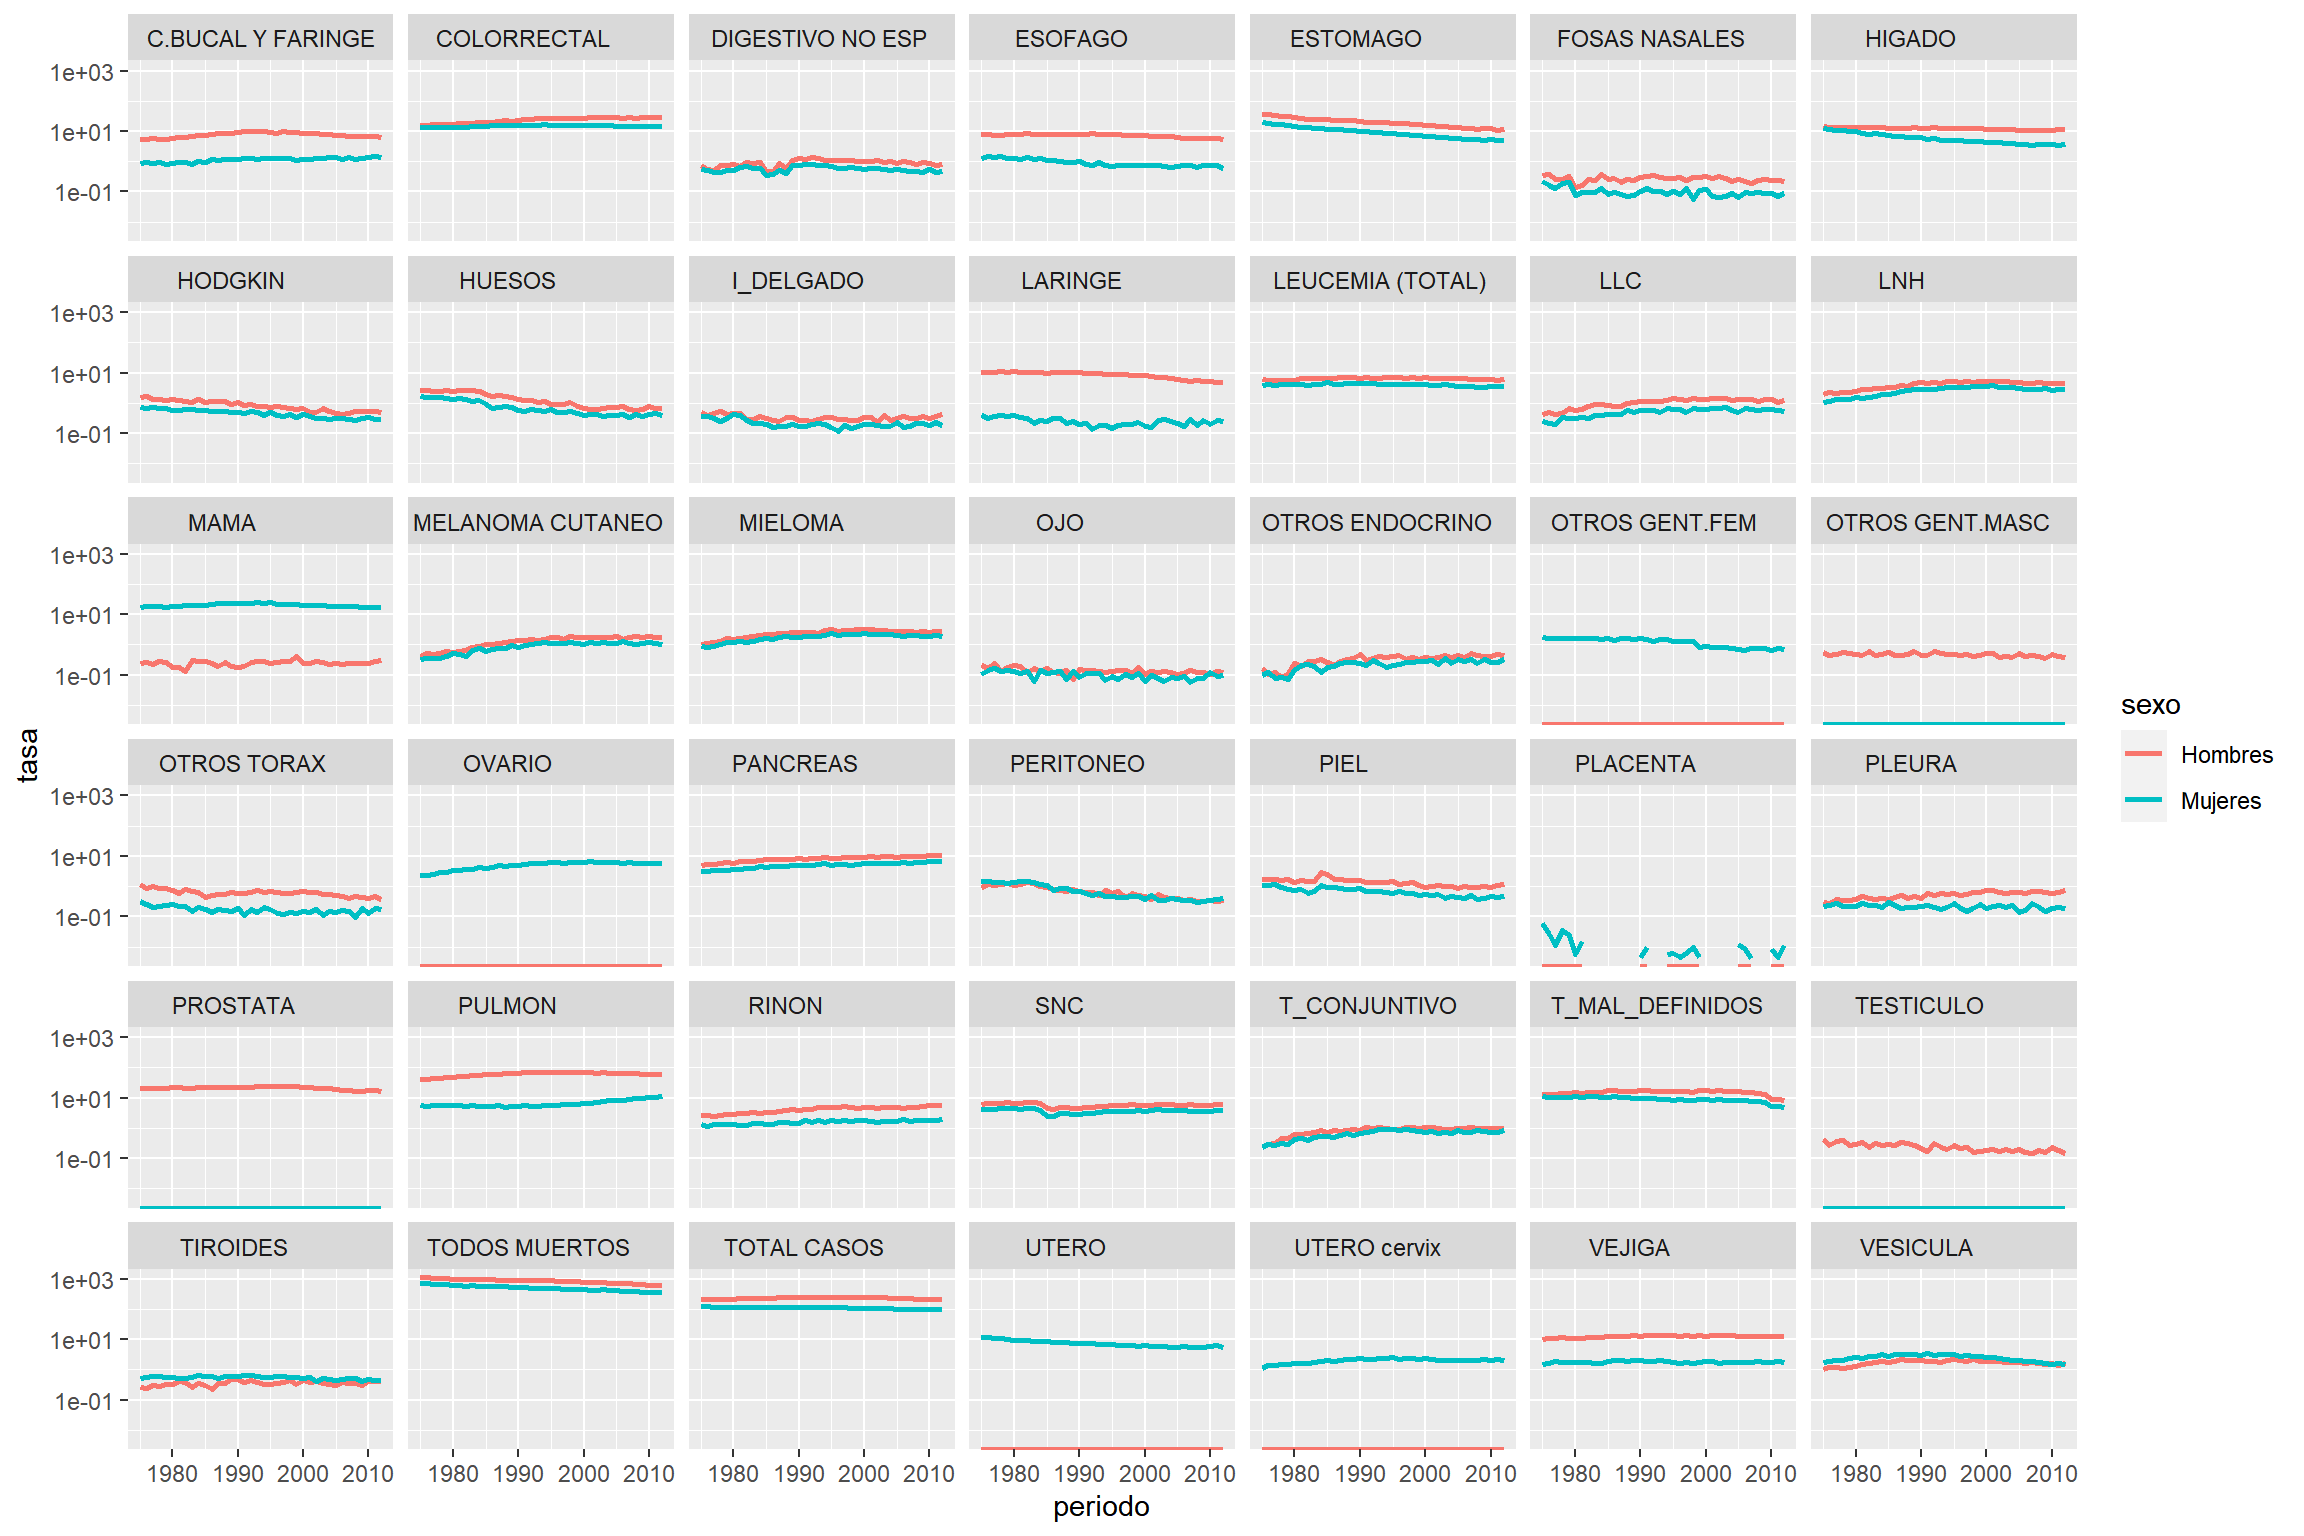
\includegraphics{graficosConR_files/figure-latex/unnamed-chunk-25-1.pdf}

\hypertarget{elementos-de-un-gruxe1fico}{%
\subsection{Elementos de un gráfico}\label{elementos-de-un-gruxe1fico}}

El gráfico anterior, se obtuvo de la siguiente manera. En primer lugar, se carga los datos de mortalidad:

\begin{Shaded}
\begin{Highlighting}[]
\FunctionTok{require}\NormalTok{(data.table)}
\FunctionTok{load}\NormalTok{(}\StringTok{"data/cancer.RDA"}\NormalTok{) }\CommentTok{\#carga los datos}
\NormalTok{cancer}
\end{Highlighting}
\end{Shaded}

\begin{verbatim}
##          sexo periodo             tumor       tasa
##    1: Hombres    1975 C.BUCAL Y FARINGE   5.541879
##    2: Hombres    1976 C.BUCAL Y FARINGE   5.512168
##    3: Hombres    1977 C.BUCAL Y FARINGE   5.827874
##    4: Hombres    1978 C.BUCAL Y FARINGE   5.323451
##    5: Hombres    1979 C.BUCAL Y FARINGE   5.461059
##   ---                                             
## 3188: Mujeres    2008 TODOS MUERTOS     385.294977
## 3189: Mujeres    2009 TODOS MUERTOS     373.009470
## 3190: Mujeres    2010 TODOS MUERTOS     359.444478
## 3191: Mujeres    2011 TODOS MUERTOS     357.461639
## 3192: Mujeres    2012 TODOS MUERTOS     359.691700
\end{verbatim}

La expresión de \texttt{ggplot2} para crear el gráfico fue:

\begin{Shaded}
\begin{Highlighting}[]
\FunctionTok{ggplot}\NormalTok{(cancer) }\SpecialCharTok{+}
  \FunctionTok{aes}\NormalTok{(}\AttributeTok{x =}\NormalTok{ periodo, }\AttributeTok{y =}\NormalTok{ tasa, }\AttributeTok{col =}\NormalTok{ sexo) }\SpecialCharTok{+}
  \FunctionTok{geom\_line}\NormalTok{(}\AttributeTok{size=}\DecValTok{1}\NormalTok{) }\SpecialCharTok{+} \FunctionTok{scale\_y\_log10}\NormalTok{() }\SpecialCharTok{+}
  \FunctionTok{facet\_wrap}\NormalTok{( }\SpecialCharTok{\textasciitilde{}}\NormalTok{ tumor) }
\end{Highlighting}
\end{Shaded}

Esta expresión combina varios elementos que discutiremos en detalle a continuación:

\begin{itemize}
\tightlist
\item
  \textbf{Datos}: siempre un ``data.frame''
\item
  \textbf{Estéticas}: elementos representables gráficamente (la posición \texttt{x} e \texttt{y}, el color, la forma, \ldots) en columnas del data.frame.
\item
  \textbf{Geometrías} (o capas): puntos, rectas, histogramas, densidades, etc. También se llaman capas porque pueden superponerse.
\item
  \textbf{Facetas}: parten un gráfico en sublienzos preservando las escalas (pequeños múltiplos)
\end{itemize}

\hypertarget{datos}{%
\subsubsection{Datos}\label{datos}}

Uno de los elementos más importantes de un gráfico son los datos que se quieren representar. Una particularidad de \texttt{ggplot2} es que solo acepta un tipo de datos: un \texttt{data.frame}.

Por otro lado, es preferible que los datos estén en un formato ``largo'' (long format), es decir, una columna para cada dimensión y una fila para cada observación.

Para ilustrar esta idea, se considera la base de datos \texttt{VADeaths} que proporciona tasas de mortalidad (por 1000 personas/año) en Virginia (1940) por grupos socio-demográficos y de edad.

\begin{tabular}{lrrrr}
\toprule
  & Rural Male & Rural Female & Urban Male & Urban Female\\
\midrule
50-54 & 11.7 & 8.7 & 15.4 & 8.4\\
55-59 & 18.1 & 11.7 & 24.3 & 13.6\\
60-64 & 26.9 & 20.3 & 37.0 & 19.3\\
65-69 & 41.0 & 30.9 & 54.6 & 35.1\\
70-74 & 66.0 & 54.3 & 71.1 & 50.0\\
\bottomrule
\end{tabular}

Antes de representar los datos, convertimos la base en un formato alargado.

\begin{Shaded}
\begin{Highlighting}[]
\FunctionTok{require}\NormalTok{(data.table)}
\NormalTok{temp}\OtherTok{=}\FunctionTok{as.data.table}\NormalTok{(VADeaths,}\AttributeTok{keep.rownames=}\ConstantTok{TRUE}\NormalTok{)}
\NormalTok{mortalidad}\OtherTok{=}\FunctionTok{melt}\NormalTok{(temp,}\AttributeTok{id.vars=}\StringTok{"rn"}\NormalTok{) }\CommentTok{\#formato alargado}
\FunctionTok{names}\NormalTok{(mortalidad) }\OtherTok{\textless{}{-}} \FunctionTok{c}\NormalTok{(}\StringTok{"edad"}\NormalTok{,}\StringTok{"grupo"}\NormalTok{,}\StringTok{"tasa"}\NormalTok{)}
\NormalTok{mortalidad}
\end{Highlighting}
\end{Shaded}

\begin{verbatim}
##      edad        grupo tasa
##  1: 50-54   Rural Male 11.7
##  2: 55-59   Rural Male 18.1
##  3: 60-64   Rural Male 26.9
##  4: 65-69   Rural Male 41.0
##  5: 70-74   Rural Male 66.0
##  6: 50-54 Rural Female  8.7
##  7: 55-59 Rural Female 11.7
##  8: 60-64 Rural Female 20.3
##  9: 65-69 Rural Female 30.9
## 10: 70-74 Rural Female 54.3
## 11: 50-54   Urban Male 15.4
## 12: 55-59   Urban Male 24.3
## 13: 60-64   Urban Male 37.0
## 14: 65-69   Urban Male 54.6
## 15: 70-74   Urban Male 71.1
## 16: 50-54 Urban Female  8.4
## 17: 55-59 Urban Female 13.6
## 18: 60-64 Urban Female 19.3
## 19: 65-69 Urban Female 35.1
## 20: 70-74 Urban Female 50.0
\end{verbatim}

\begin{Shaded}
\begin{Highlighting}[]
\NormalTok{p }\OtherTok{\textless{}{-}} \FunctionTok{ggplot}\NormalTok{(mortalidad)}
\end{Highlighting}
\end{Shaded}

El código anterior crea un objeto, \texttt{p} que viene a ser un proto-gráfico: contiene los datos que vamos a utilizar, los del conjunto de datos \texttt{mortalidad}. Obviamente, el código anterior es insuficiente para crear un gráfico: aún no hemos indicado qué queremos hacer con \texttt{mortalidad}.

\hypertarget{estuxe9ticas-aes}{%
\subsubsection{\texorpdfstring{Estéticas (\texttt{aes})}{Estéticas (aes)}}\label{estuxe9ticas-aes}}

En un conjunto de datos hay columnas: edad, altura, ingresos, temperatura, etc. En un gráfico hay, en la terminología de \texttt{ggplot2}, \emph{aesthetic}. Estéticas son, por ejemplo, la distancia horizontal o vertical, el color, la forma (de un punto), el tamaño (de un punto o el grosor de una línea), etc.

\begin{Shaded}
\begin{Highlighting}[]
\NormalTok{p }\OtherTok{\textless{}{-}}\NormalTok{ p }\SpecialCharTok{+} \FunctionTok{aes}\NormalTok{(}\AttributeTok{x =}\NormalTok{ edad, }\AttributeTok{y =}\NormalTok{ tasa, }\AttributeTok{colour =}\NormalTok{ grupo)}
\end{Highlighting}
\end{Shaded}

se están añadiendo a \texttt{p} información sobre las estéticas que tiene que utilizar y qué variables de \texttt{mortalidad} tiene que utilizar:

\begin{itemize}
\tightlist
\item
  La abscisa \texttt{x}, vendrá dada por el grupo de edad.
\item
  La ordenada \texttt{y}, por la tasa de mortalidad.
\item
  El color, por el grupo socio-demográfico.
\end{itemize}

Al \emph{protográfico} se le han sumado las estéticas. En las secciones siguientes se le \emph{sumarán} otros elementos adicionales. Lo importante es recordar cómo la suma es el signo que combina los elementos que componen el lenguaje de los gráficos.

De todos modos, es habitual combinar ambos pasos en una única expresión

\begin{Shaded}
\begin{Highlighting}[]
\NormalTok{p }\OtherTok{\textless{}{-}} \FunctionTok{ggplot}\NormalTok{(mortalidad, }\FunctionTok{aes}\NormalTok{(}\AttributeTok{x =}\NormalTok{ edad, }\AttributeTok{y =}\NormalTok{ tasa, }\AttributeTok{colour =}\NormalTok{ grupo))}
\end{Highlighting}
\end{Shaded}

El objeto \texttt{p} resultante aún no es un gráfico ni se puede representar. Le faltan capas, que es el objeto de la siguiente sección. No obstante, se puede inspeccionar la relación (o \emph{mapeo}) entre estéticas y columnas de los datos:

\begin{Shaded}
\begin{Highlighting}[]
\NormalTok{p}\SpecialCharTok{$}\NormalTok{mapping}
\end{Highlighting}
\end{Shaded}

\begin{verbatim}
## Aesthetic mapping: 
## * `x`      -> `edad`
## * `y`      -> `tasa`
## * `colour` -> `grupo`
\end{verbatim}

¿Cuántas estéticas existen? Alrededor de una docena, aunque se utilizan, generalmente, menos:

\begin{itemize}
\tightlist
\item
  \texttt{x} e \texttt{y}, coordenadas horizontal y vertical.
\item
  \texttt{colour}, para el color.
\item
  \texttt{size}, para el tamaño.
\item
  \texttt{shape}, que indica la forma de los puntos (cuadrados, triángulos, etc.) de los puntos o del trazo (continuo, punteado) de las líneas.
\item
  \texttt{alpha} para la transparencia: los valores más altos tendrían formas opacas y los más bajos, casi transparentes. También muy útil para el solapamiento de puntos.
\item
  \texttt{fill}, para el color de relleno de las formas sólidas (barras, etc.).
\end{itemize}

\begin{nota}
Hay que advertir que NO todas las \emph{estéticas} tienen la misma
potencia en un gráfico. El ojo humano percibe fácilmente longitudes
distintas. Pero tiene problemas para comparar áreas (que es lo que
regula la estética \texttt{size}) o intensidades de color. Se recomienda
usar las estéticas más potentes para representar las variables más
importantes.
\end{nota}

\hypertarget{capas-geoms}{%
\subsubsection{\texorpdfstring{Capas (\texttt{geoms})}{Capas (geoms)}}\label{capas-geoms}}

Las capas (o \texttt{geoms} para \texttt{ggplot2}) son los verbos del lenguaje de los gráficos. Indican qué hacer con los datos y las estéticas elegidas, cómo representarlos en un lienzo:

\begin{Shaded}
\begin{Highlighting}[]
\NormalTok{p }\OtherTok{\textless{}{-}}\NormalTok{ p }\SpecialCharTok{+} \FunctionTok{geom\_point}\NormalTok{()}
\NormalTok{p}
\end{Highlighting}
\end{Shaded}

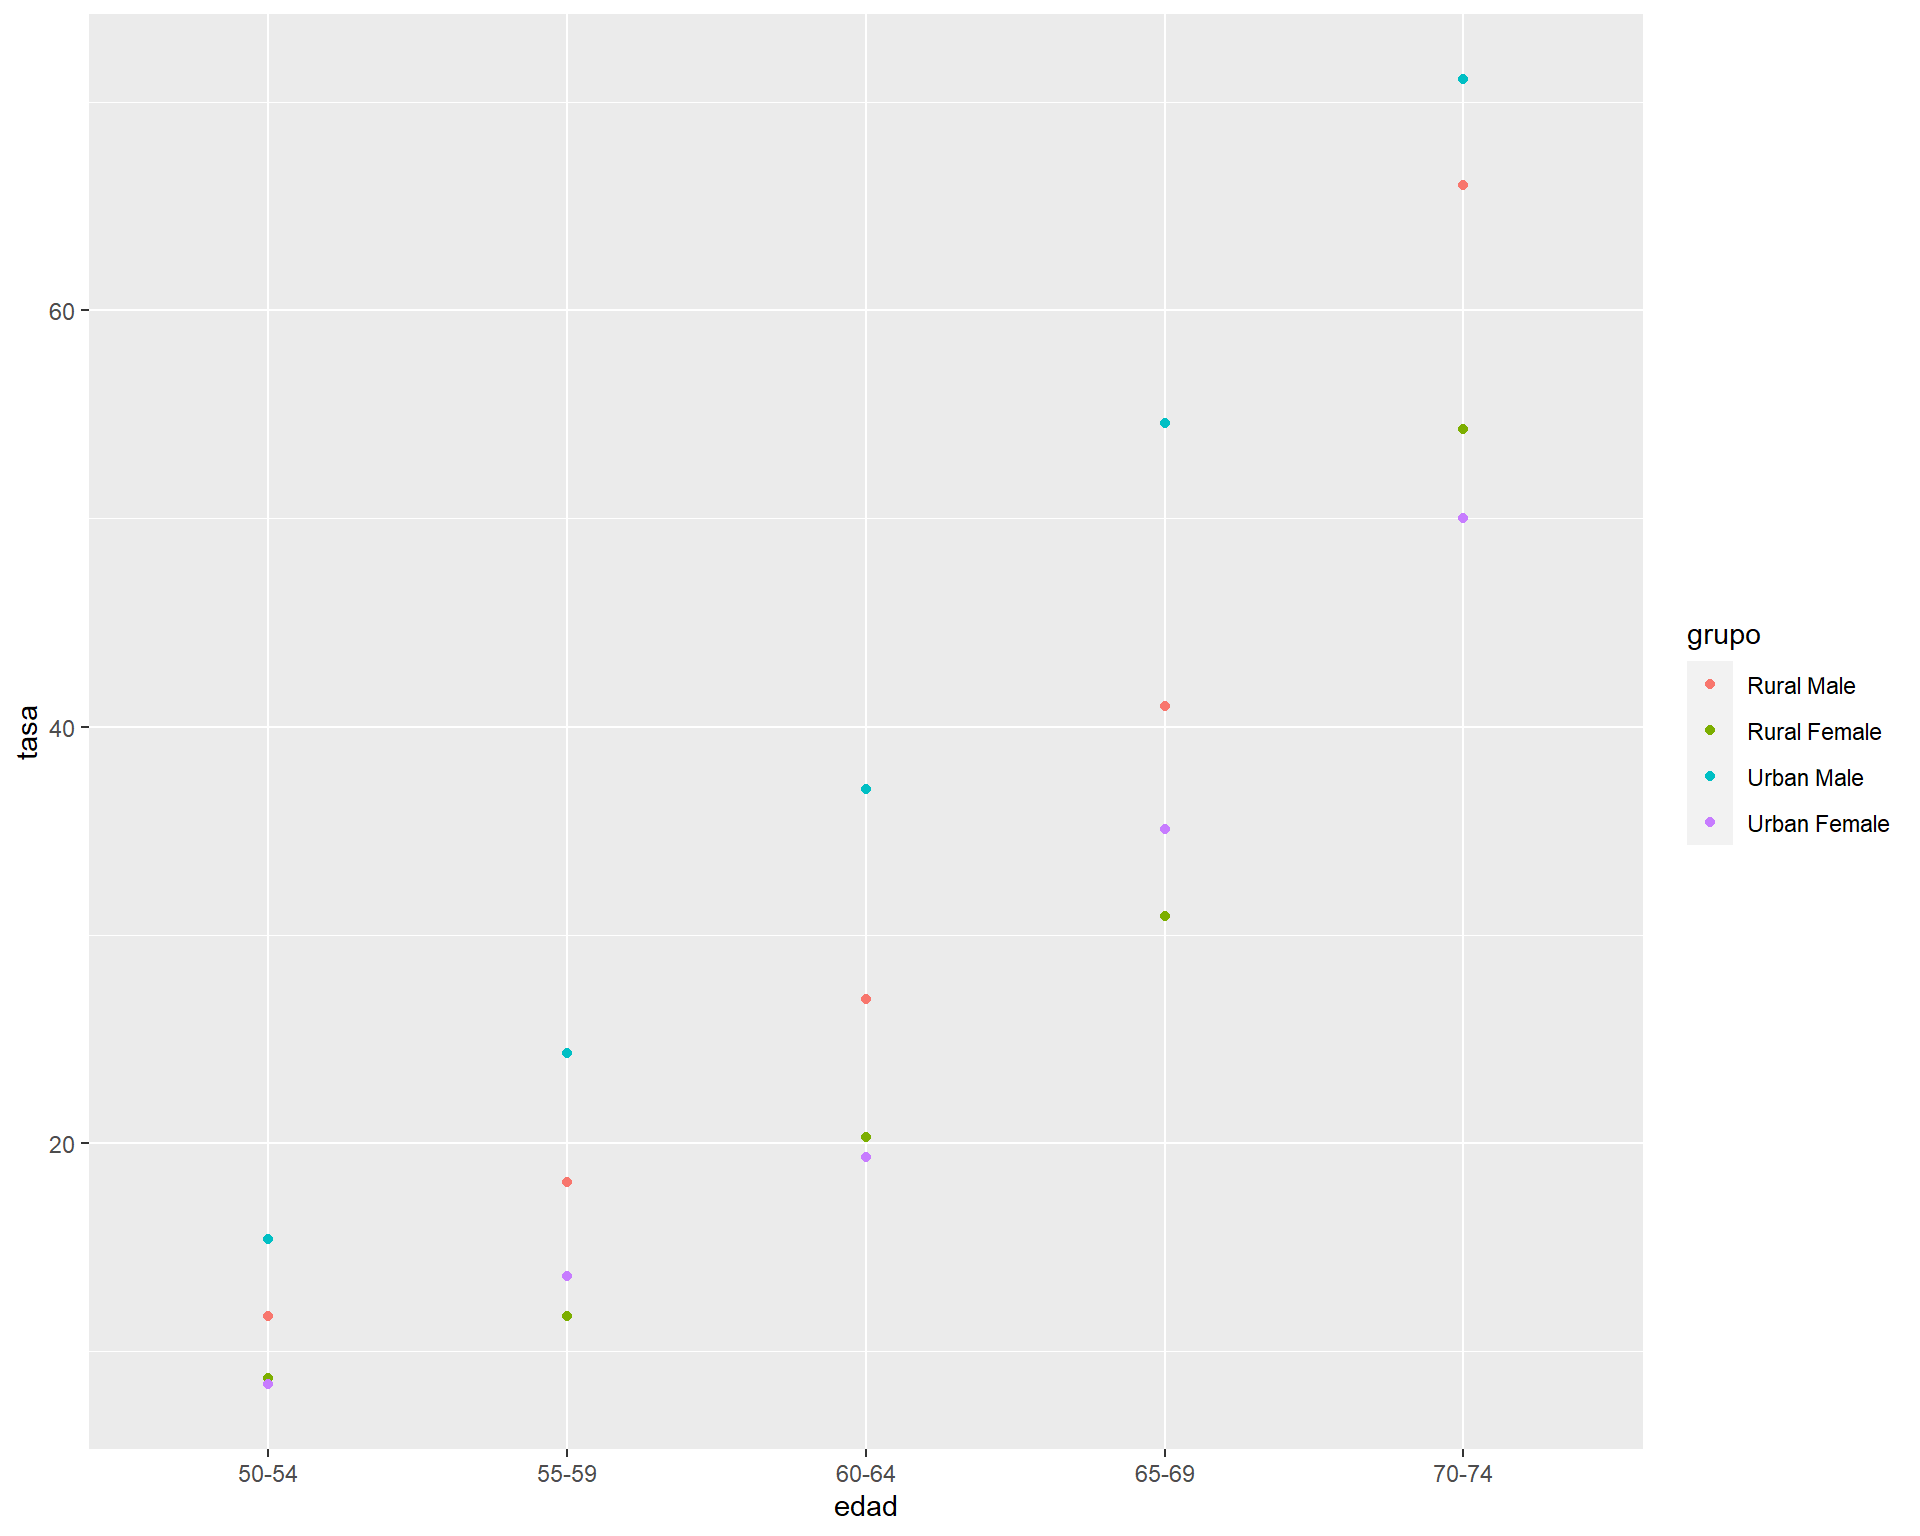
\includegraphics{graficosConR_files/figure-latex/unnamed-chunk-35-1.pdf}

Una vez añadida una capa al gráfico, este puede pintarse (que es lo que ocurre al llamar a \texttt{p}). Se obtiene el mismo resultado haciendo, en una única línea,

\begin{Shaded}
\begin{Highlighting}[]
\FunctionTok{ggplot}\NormalTok{(mortalidad, }\FunctionTok{aes}\NormalTok{(}\AttributeTok{x =}\NormalTok{ edad, }\AttributeTok{y =}\NormalTok{ tasa, }\AttributeTok{colour =}\NormalTok{ grupo)) }\SpecialCharTok{+} \FunctionTok{geom\_point}\NormalTok{()}
\end{Highlighting}
\end{Shaded}

Una característica de las capas, y de ahí su nombre, es que pueden superponerse. Por ejemplo,

\begin{Shaded}
\begin{Highlighting}[]
\FunctionTok{ggplot}\NormalTok{(mortalidad, }\FunctionTok{aes}\NormalTok{(}\AttributeTok{x =}\NormalTok{ edad, }\AttributeTok{y =}\NormalTok{ tasa, }\AttributeTok{colour =}\NormalTok{ grupo, }\AttributeTok{group=}\NormalTok{ grupo)) }\SpecialCharTok{+} 
  \FunctionTok{geom\_point}\NormalTok{() }\SpecialCharTok{+} \FunctionTok{geom\_line}\NormalTok{()}
\end{Highlighting}
\end{Shaded}

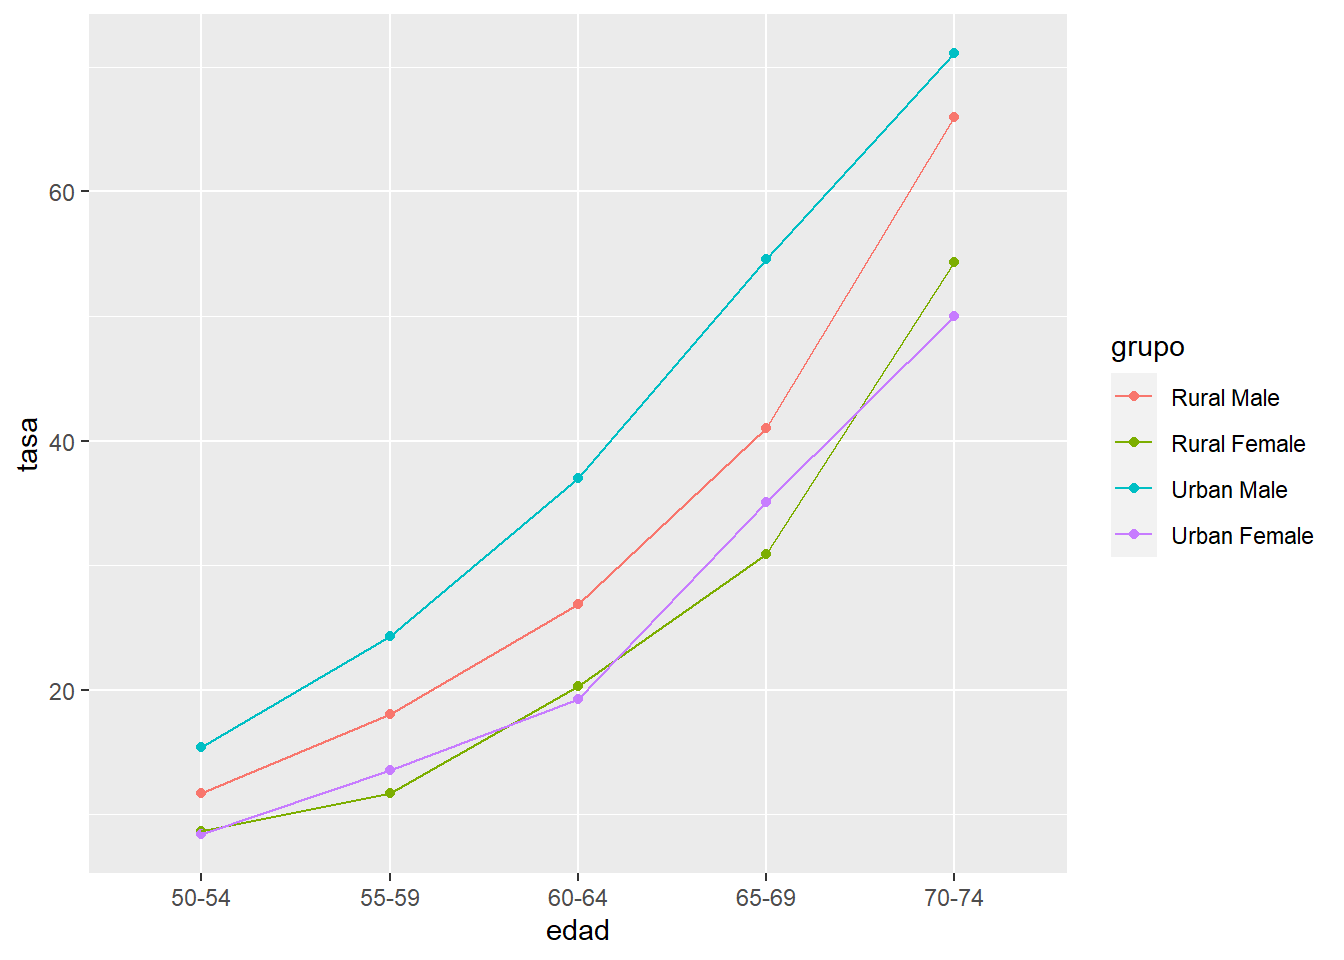
\includegraphics{graficosConR_files/figure-latex/unnamed-chunk-37-1.pdf}

\begin{Shaded}
\begin{Highlighting}[]
\CommentTok{\# Se requiere la estética \textasciigrave{}group\textasciigrave{} para conectar los puntos de una linea cuando la variable en abscisa es un factor.}
\end{Highlighting}
\end{Shaded}

Existen muchos tipos de capas. Los más usuales son \texttt{geom\_point}, \texttt{geom\_line}, \texttt{geom\_histogram}, \texttt{geom\_bar} y \texttt{geom\_boxplot} (ver las página \texttt{https://ggplot2.tidyverse.org/reference/}) para una lista actualizada.

Abajo una representación mediante un diagrama de barra de los datos anteriores:

\begin{Shaded}
\begin{Highlighting}[]
\FunctionTok{ggplot}\NormalTok{(mortalidad, }\FunctionTok{aes}\NormalTok{(}\AttributeTok{x =}\NormalTok{ edad, }\AttributeTok{y =}\NormalTok{ tasa, }\AttributeTok{fill =}\NormalTok{ grupo)) }\SpecialCharTok{+} 
  \FunctionTok{geom\_bar}\NormalTok{(}\AttributeTok{stat=}\StringTok{"identity"}\NormalTok{,}\AttributeTok{position=}\StringTok{"dodge"}\NormalTok{)}
\end{Highlighting}
\end{Shaded}

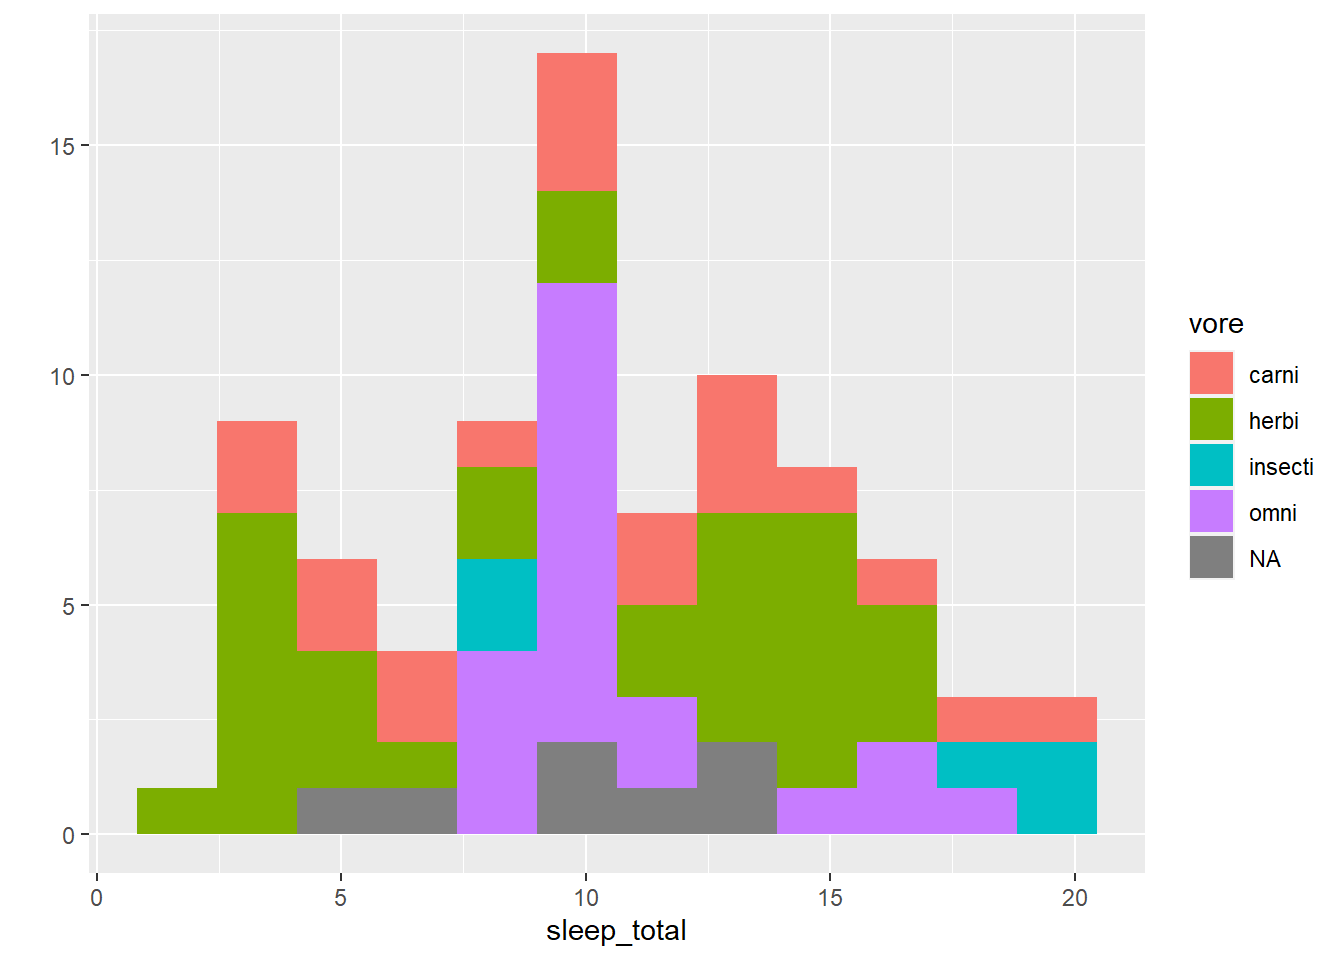
\includegraphics{graficosConR_files/figure-latex/unnamed-chunk-38-1.pdf}

\begin{ej}
Elaborar el siguientes gráfico sobre la evolución del paro en España.
Utilizar la capa \texttt{geom\_smooth} para suavizar la tendencia y la
estética \texttt{linetype} para distintos tipos de curvas.
\end{ej}

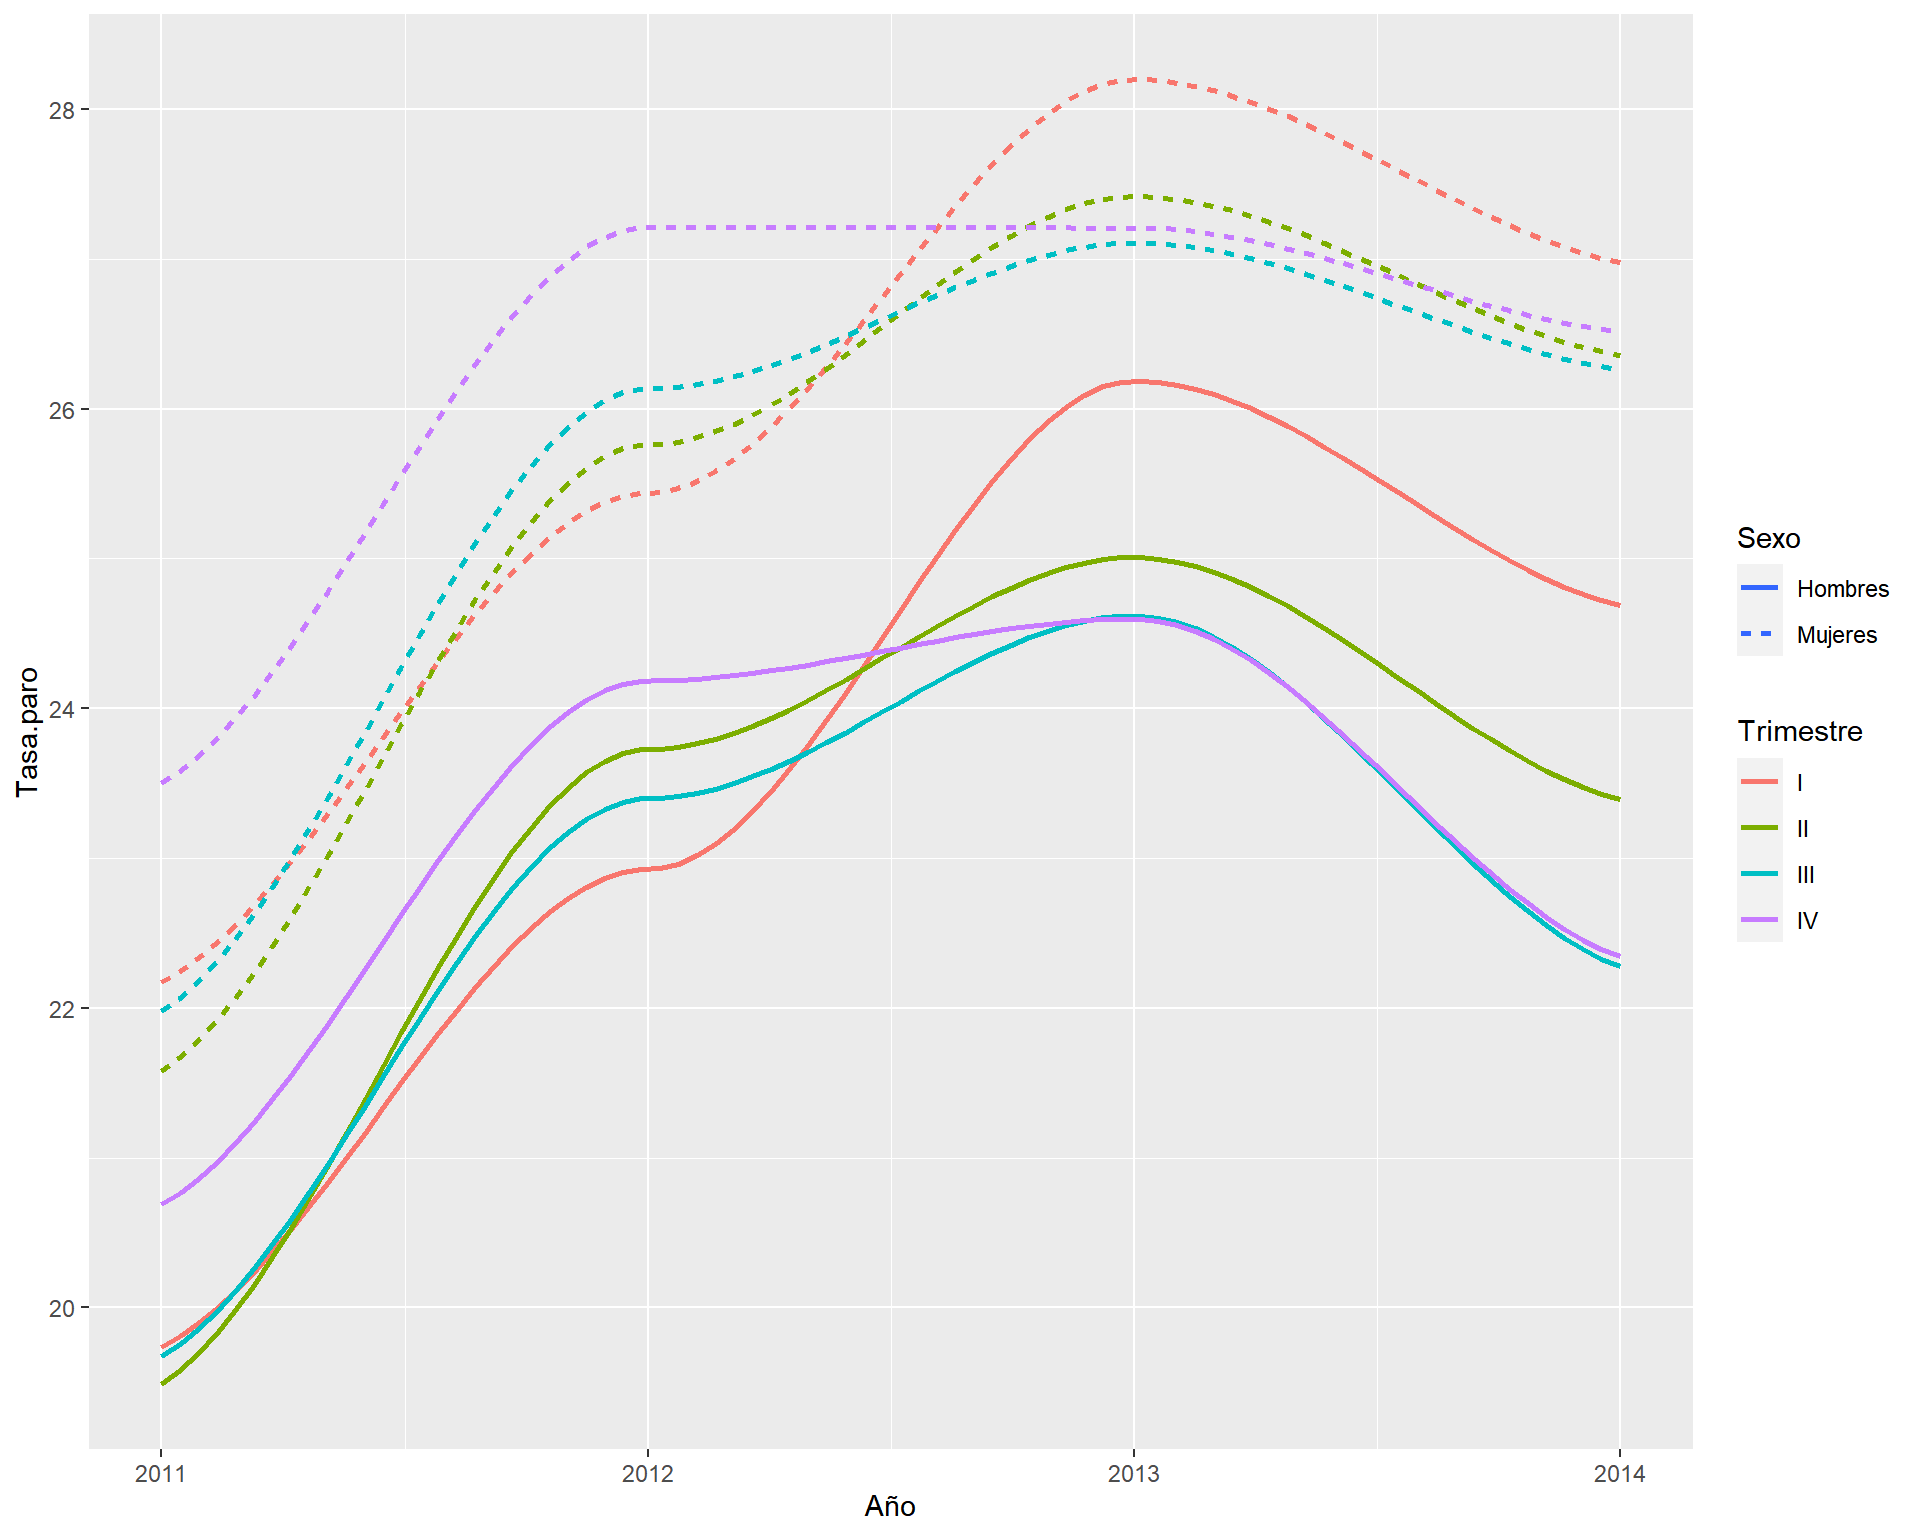
\includegraphics{graficosConR_files/figure-latex/unnamed-chunk-40-1.pdf}

\begin{ej}
Elaborar un gráfico sobre la evolución del número de hospitalización por
COVID en España. Se podría utilizar la capa \texttt{geom\_area} y la
estética \texttt{fill} para distinguir mejor los distintos grupos de
edad.
\end{ej}

\hypertarget{facetas}{%
\subsubsection{Facetas}\label{facetas}}

Las facetas permiten subdividir un gráfico y suele ser un recurso muy eficiente para describir el comportamiento de una variable en función de otra variable categórica. Así por ejemplo, con los datos de mortalidad,

\begin{Shaded}
\begin{Highlighting}[]
\FunctionTok{ggplot}\NormalTok{(mortalidad, }\FunctionTok{aes}\NormalTok{(}\AttributeTok{x =}\NormalTok{ edad, }\AttributeTok{y =}\NormalTok{ tasa)) }\SpecialCharTok{+} 
  \FunctionTok{geom\_bar}\NormalTok{(}\AttributeTok{stat=}\StringTok{"identity"}\NormalTok{) }\SpecialCharTok{+}
  \FunctionTok{facet\_grid}\NormalTok{(}\SpecialCharTok{\textasciitilde{}}\NormalTok{grupo)}
\end{Highlighting}
\end{Shaded}

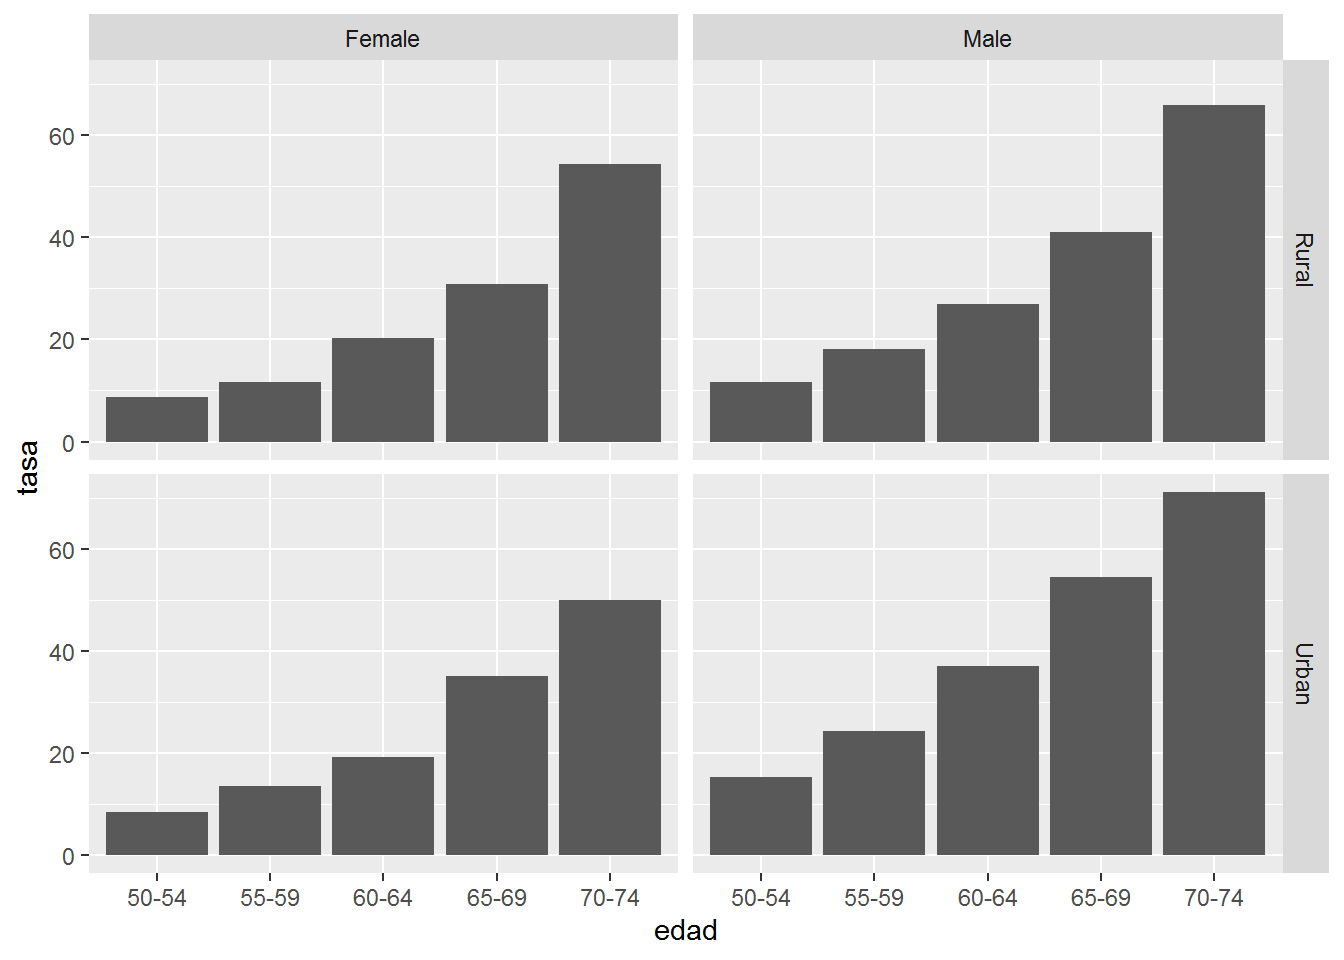
\includegraphics{graficosConR_files/figure-latex/unnamed-chunk-42-1.pdf}

crea tres gráficos dispuestos horizontalmente que comparan la relación entre la anchura y la longitud del pétalo de las tres especies de iris. Una característica de estos gráficos, que es crítica para poder hacer comparaciones adecuadas, es que comparten ejes.

Los gráficos podrían disponerse verticalmente reemplazando \texttt{facet\_grid(\textasciitilde{}grupo)} por \texttt{facet\_grid(grupo\textasciitilde{})} en el código anterior. Además, se puede subdividir el lienzo por dos (¡o más!) variables así:

\begin{Shaded}
\begin{Highlighting}[]
\NormalTok{mortalidad[,}\FunctionTok{c}\NormalTok{(}\StringTok{"zone"}\NormalTok{, }\StringTok{"sex"}\NormalTok{)}\SpecialCharTok{:}\ErrorTok{=} \FunctionTok{tstrsplit}\NormalTok{(grupo, }\StringTok{" "}\NormalTok{)]}
\FunctionTok{ggplot}\NormalTok{(mortalidad, }\FunctionTok{aes}\NormalTok{(}\AttributeTok{x =}\NormalTok{ edad, }\AttributeTok{y =}\NormalTok{ tasa)) }\SpecialCharTok{+} 
  \FunctionTok{geom\_bar}\NormalTok{(}\AttributeTok{stat=}\StringTok{"identity"}\NormalTok{) }\SpecialCharTok{+}
  \FunctionTok{facet\_grid}\NormalTok{(zone }\SpecialCharTok{\textasciitilde{}}\NormalTok{ sex)}
\end{Highlighting}
\end{Shaded}

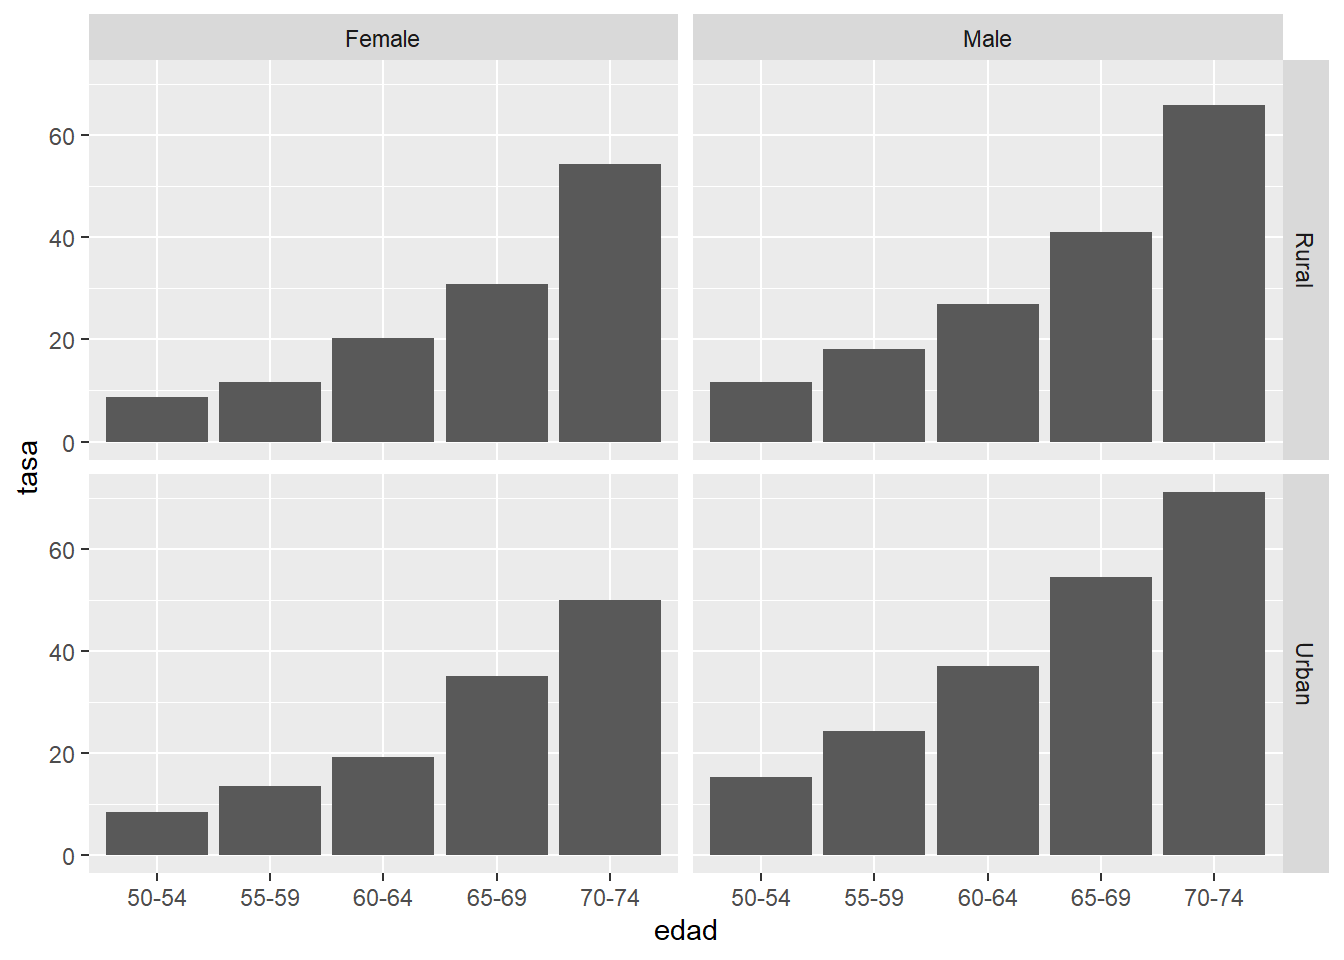
\includegraphics{graficosConR_files/figure-latex/unnamed-chunk-43-1.pdf}

\begin{ej}
Elaborar los siguientes gráficos sobre la evolución del paro (NOta: para
el segundo gráfico, limitar la base a las provincias de Zaragoza,
Huesca, Teruel.)
\end{ej}

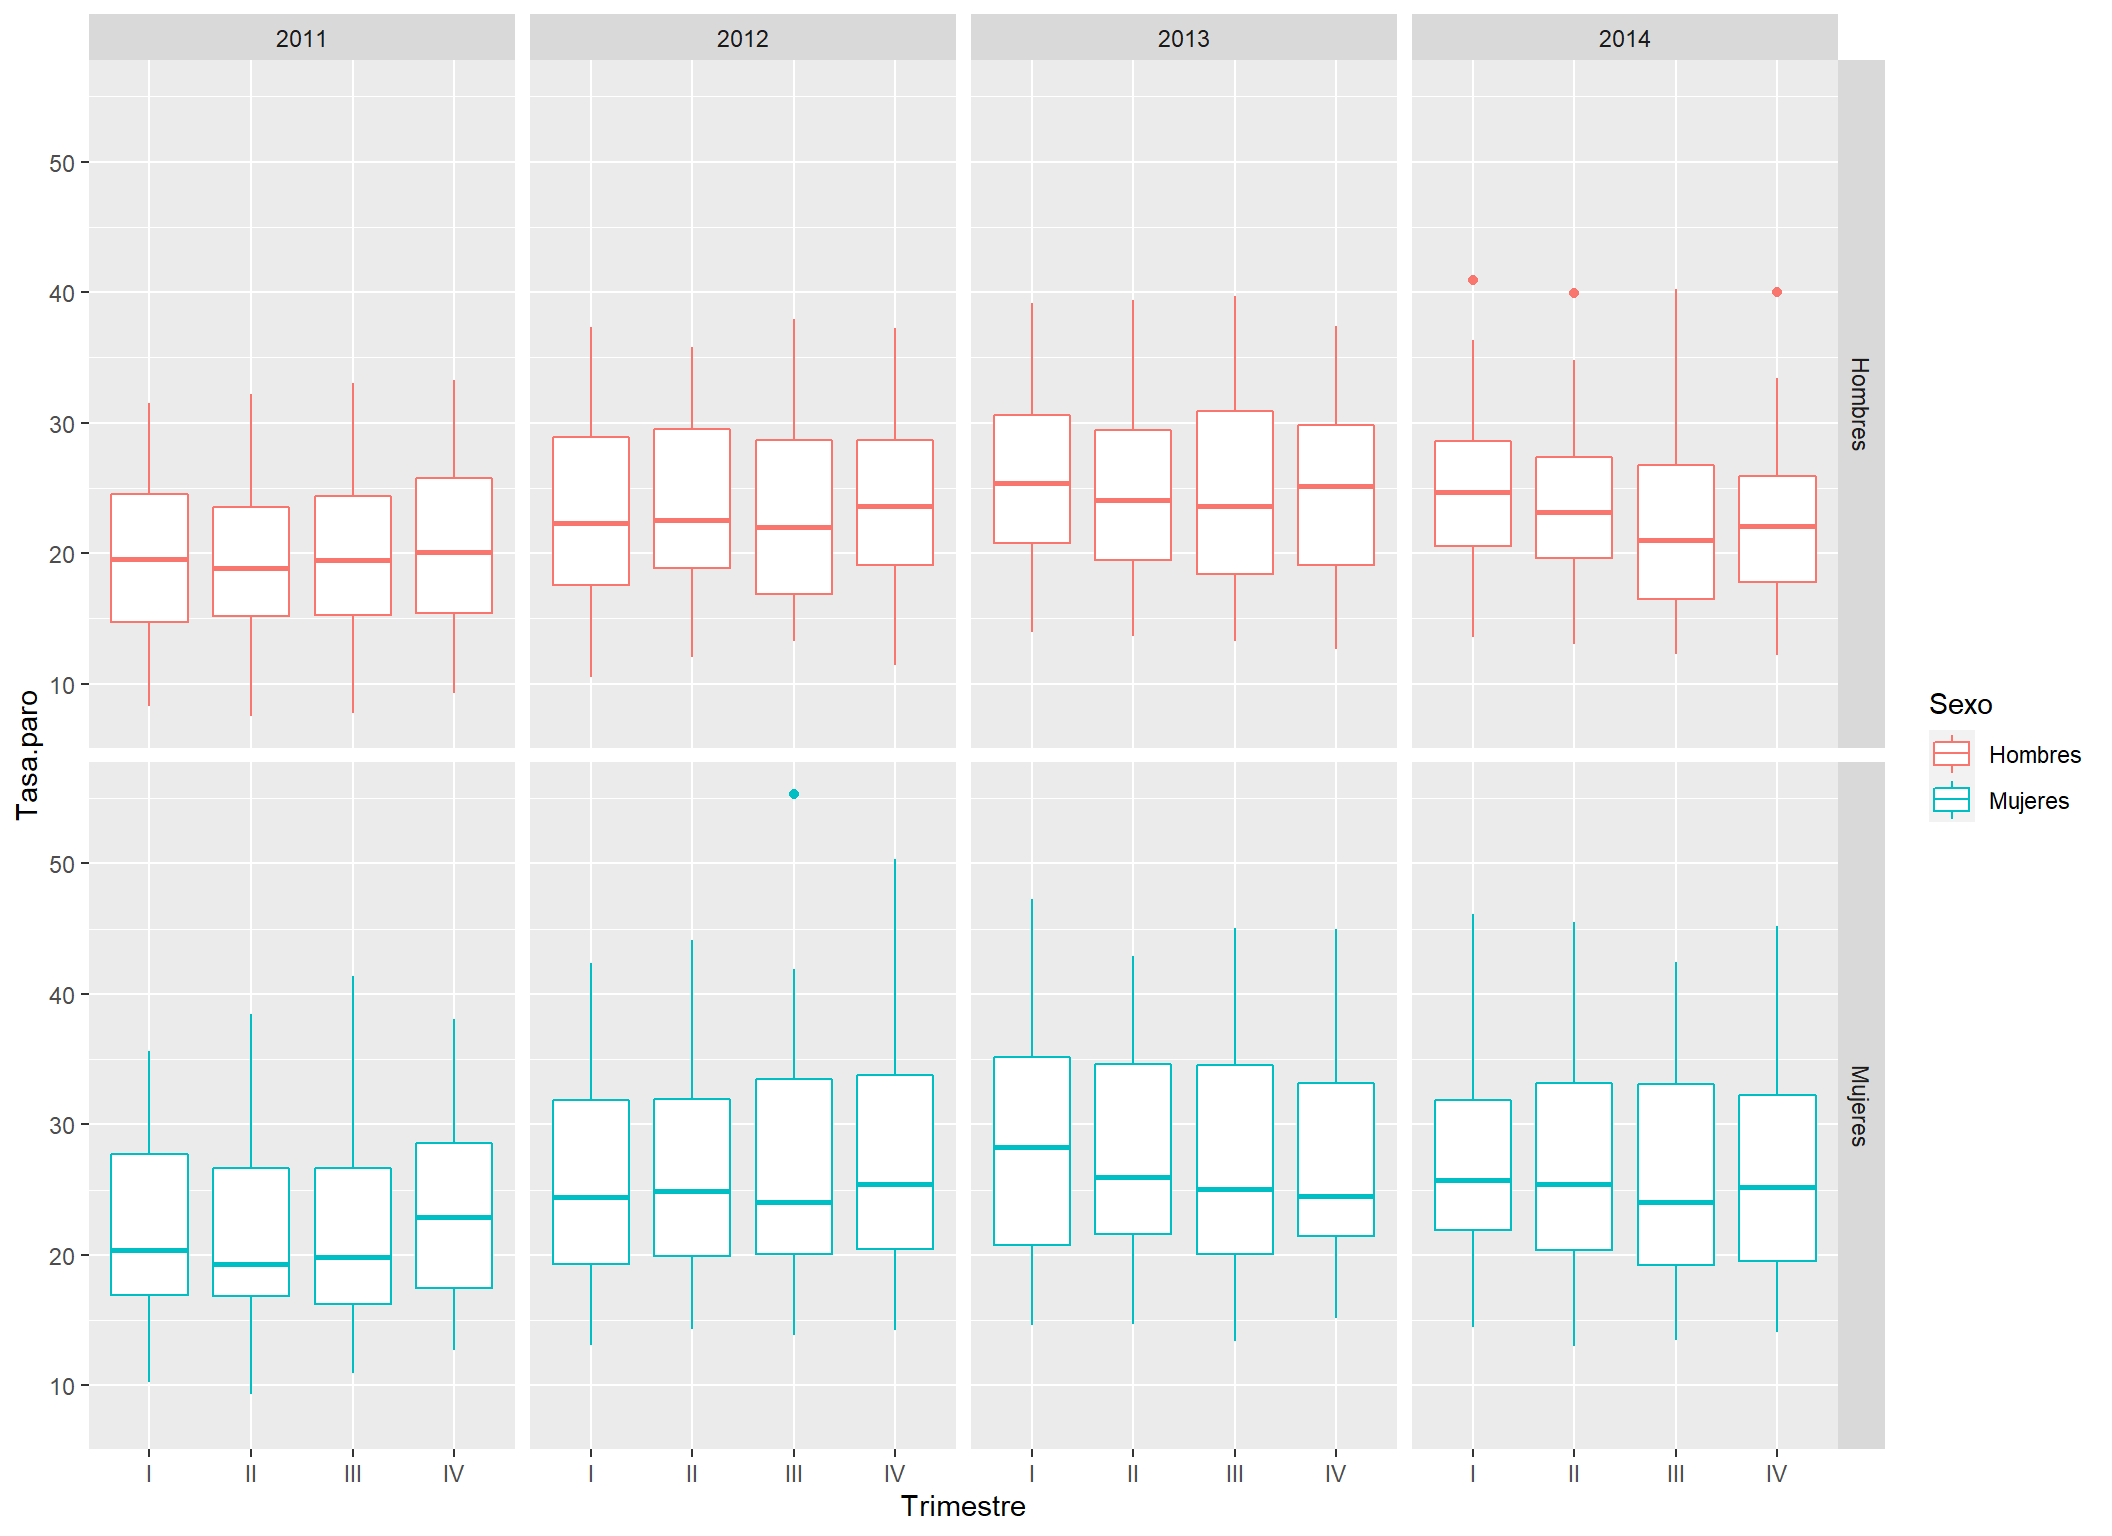
\includegraphics{graficosConR_files/figure-latex/unnamed-chunk-45-1.pdf} 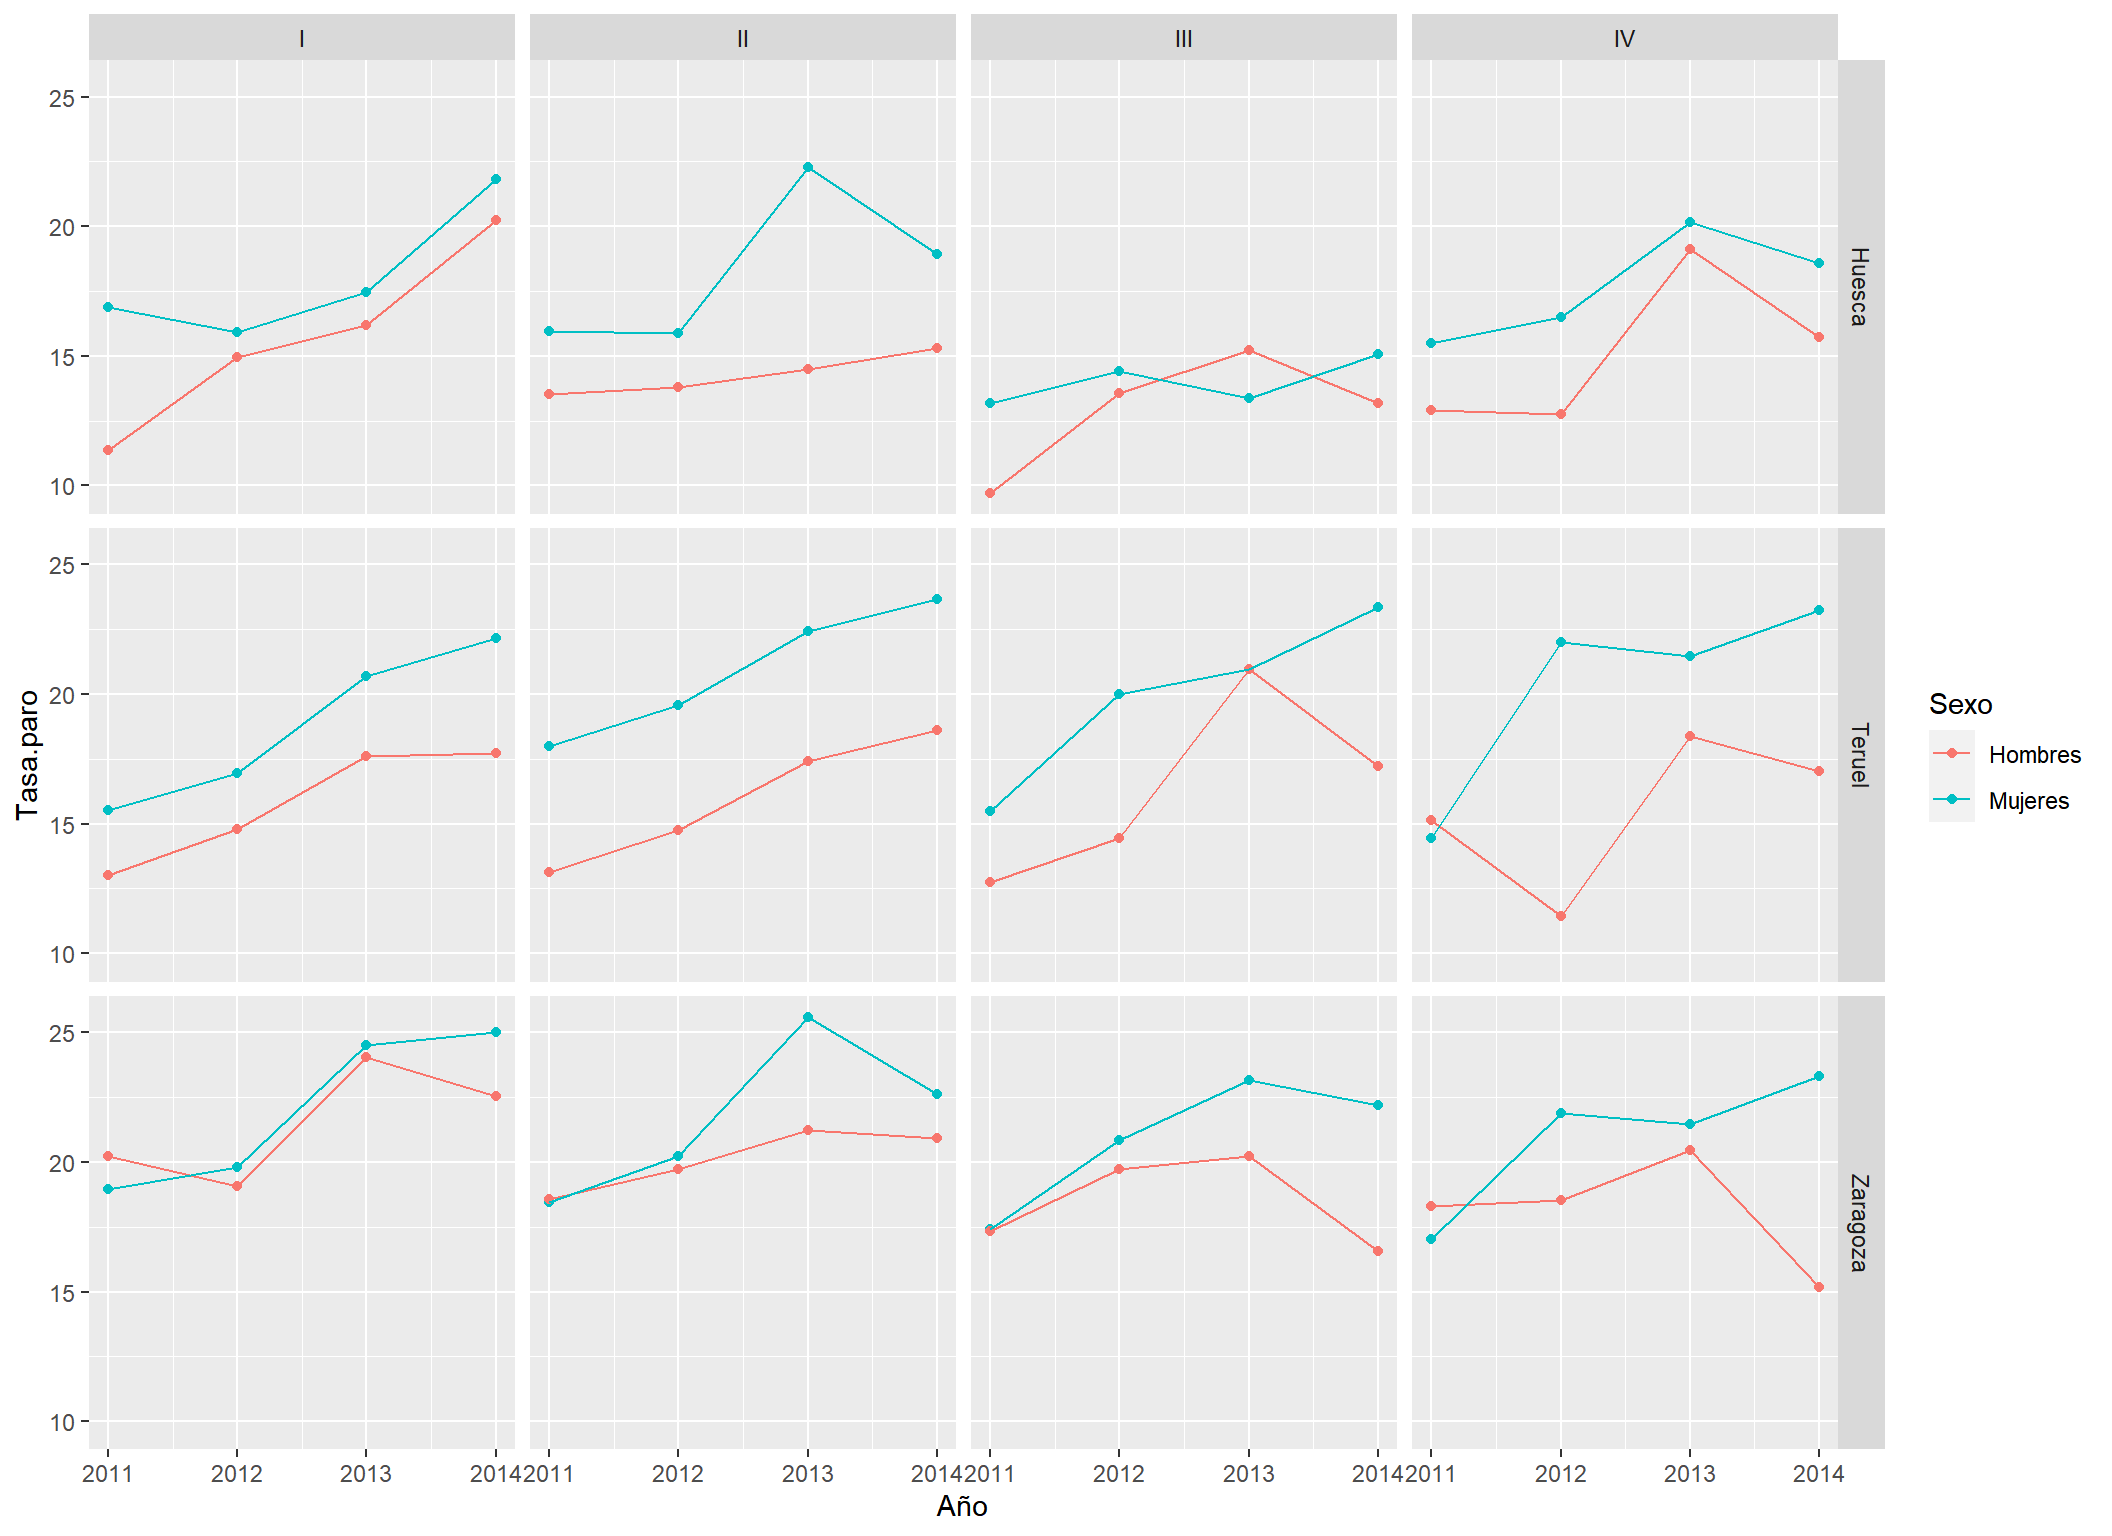
\includegraphics{graficosConR_files/figure-latex/unnamed-chunk-45-2.pdf}

En caso de haber muchas categorías (p.e., todas las provincias), puede usarse la función \texttt{facet\_wrap} para distribuir las sub-gráficas en una cuadrícula (ver gráfico a principio de la sección).

\hypertarget{toque-final}{%
\subsubsection{Toque final}\label{toque-final}}

\hypertarget{etiquetas}{%
\paragraph{Etiquetas}\label{etiquetas}}

Las estéticas se pueden etiquetar con la función \texttt{labs}. Además, se le puede añadir un título al gráfico usando la función \texttt{ggtitle}. Por ejemplo, en el gráfico anterior se pueden re-etiquetar los ejes y la leyenda escribiendo

\begin{Shaded}
\begin{Highlighting}[]
\NormalTok{obesidad}\OtherTok{\textless{}{-}}\FunctionTok{fread}\NormalTok{(}\StringTok{"data/obesidad.csv"}\NormalTok{)}
\NormalTok{p}\OtherTok{\textless{}{-}}\FunctionTok{ggplot}\NormalTok{(obesidad,}\FunctionTok{aes}\NormalTok{(}\AttributeTok{x=}\NormalTok{renta,}\AttributeTok{y=}\NormalTok{imc,}\AttributeTok{color=}\NormalTok{region))}\SpecialCharTok{+}\FunctionTok{geom\_smooth}\NormalTok{(}\AttributeTok{method=}\StringTok{"lm"}\NormalTok{)}
\NormalTok{p }\SpecialCharTok{+} \FunctionTok{ggtitle}\NormalTok{(}\StringTok{"Relación entre Indice de Masa Corporal (IMC) y renta"}\NormalTok{) }\SpecialCharTok{+} 
        \FunctionTok{labs}\NormalTok{(}\AttributeTok{x =} \StringTok{"Renta (en miles de dolares por año)"}\NormalTok{, }\AttributeTok{y =} \FunctionTok{quote}\NormalTok{(}\FunctionTok{IMC}\NormalTok{ (kg}\SpecialCharTok{/}\NormalTok{m)), }\AttributeTok{color =} \StringTok{"Continente"}\NormalTok{)}
\end{Highlighting}
\end{Shaded}

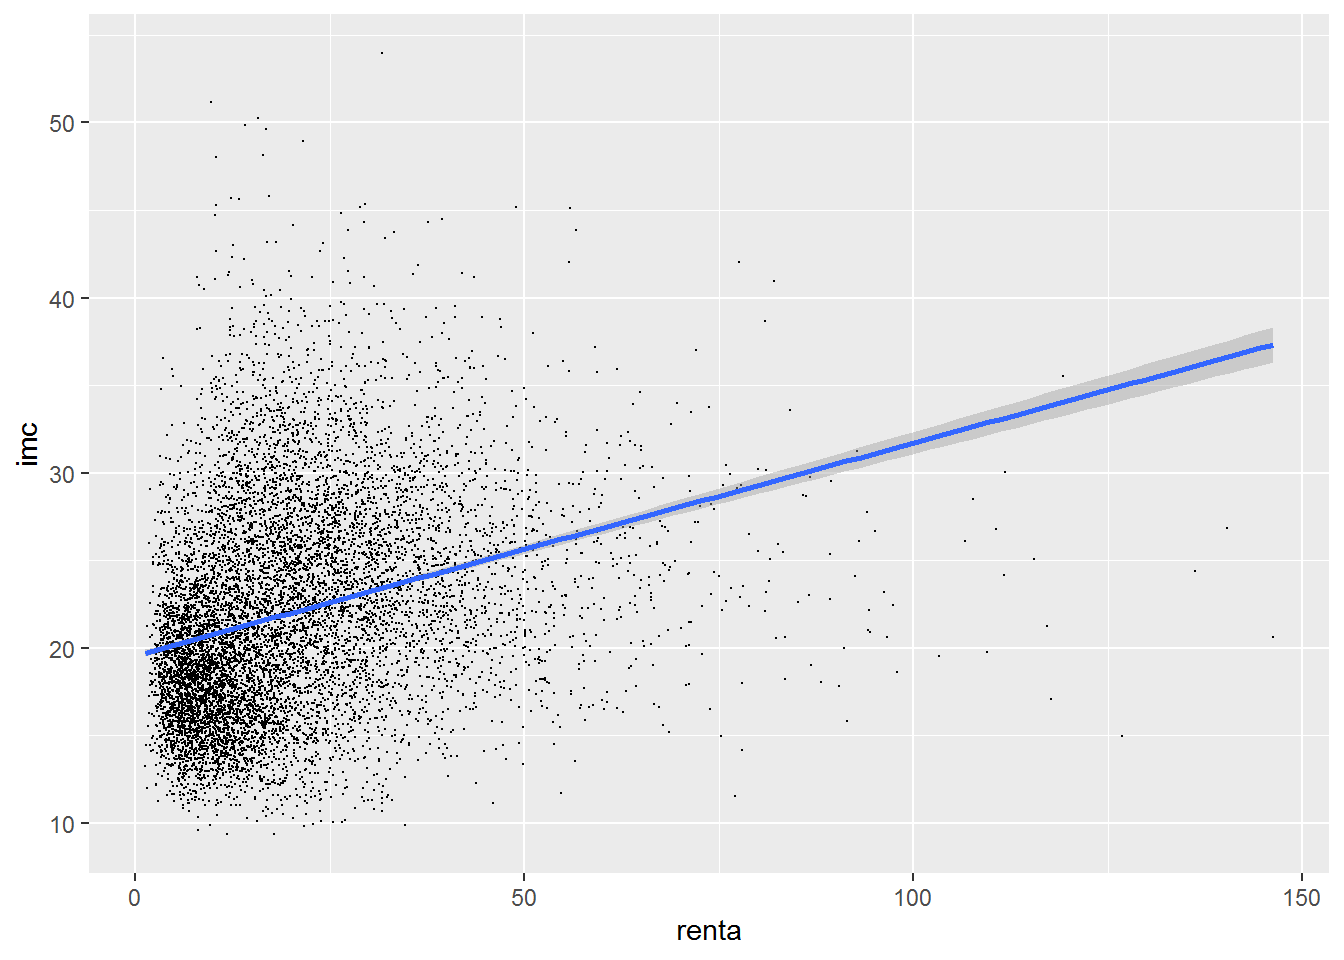
\includegraphics{graficosConR_files/figure-latex/unnamed-chunk-46-1.pdf}

\hypertarget{escalas}{%
\paragraph{Escalas}\label{escalas}}

Las escalas de las estéticas pueden ser modificadas para mejorar la claridad del gráfico.

\begin{Shaded}
\begin{Highlighting}[]
\NormalTok{p}\OtherTok{\textless{}{-}}\FunctionTok{ggplot}\NormalTok{(obesidad,}\FunctionTok{aes}\NormalTok{(}\AttributeTok{x=}\NormalTok{renta,}\AttributeTok{y=}\NormalTok{imc))}\SpecialCharTok{+}\FunctionTok{geom\_point}\NormalTok{(}\AttributeTok{size=}\NormalTok{.}\DecValTok{1}\NormalTok{)}\SpecialCharTok{+}\FunctionTok{geom\_smooth}\NormalTok{(}\AttributeTok{method=}\StringTok{"lm"}\NormalTok{)}
\NormalTok{p }
\end{Highlighting}
\end{Shaded}

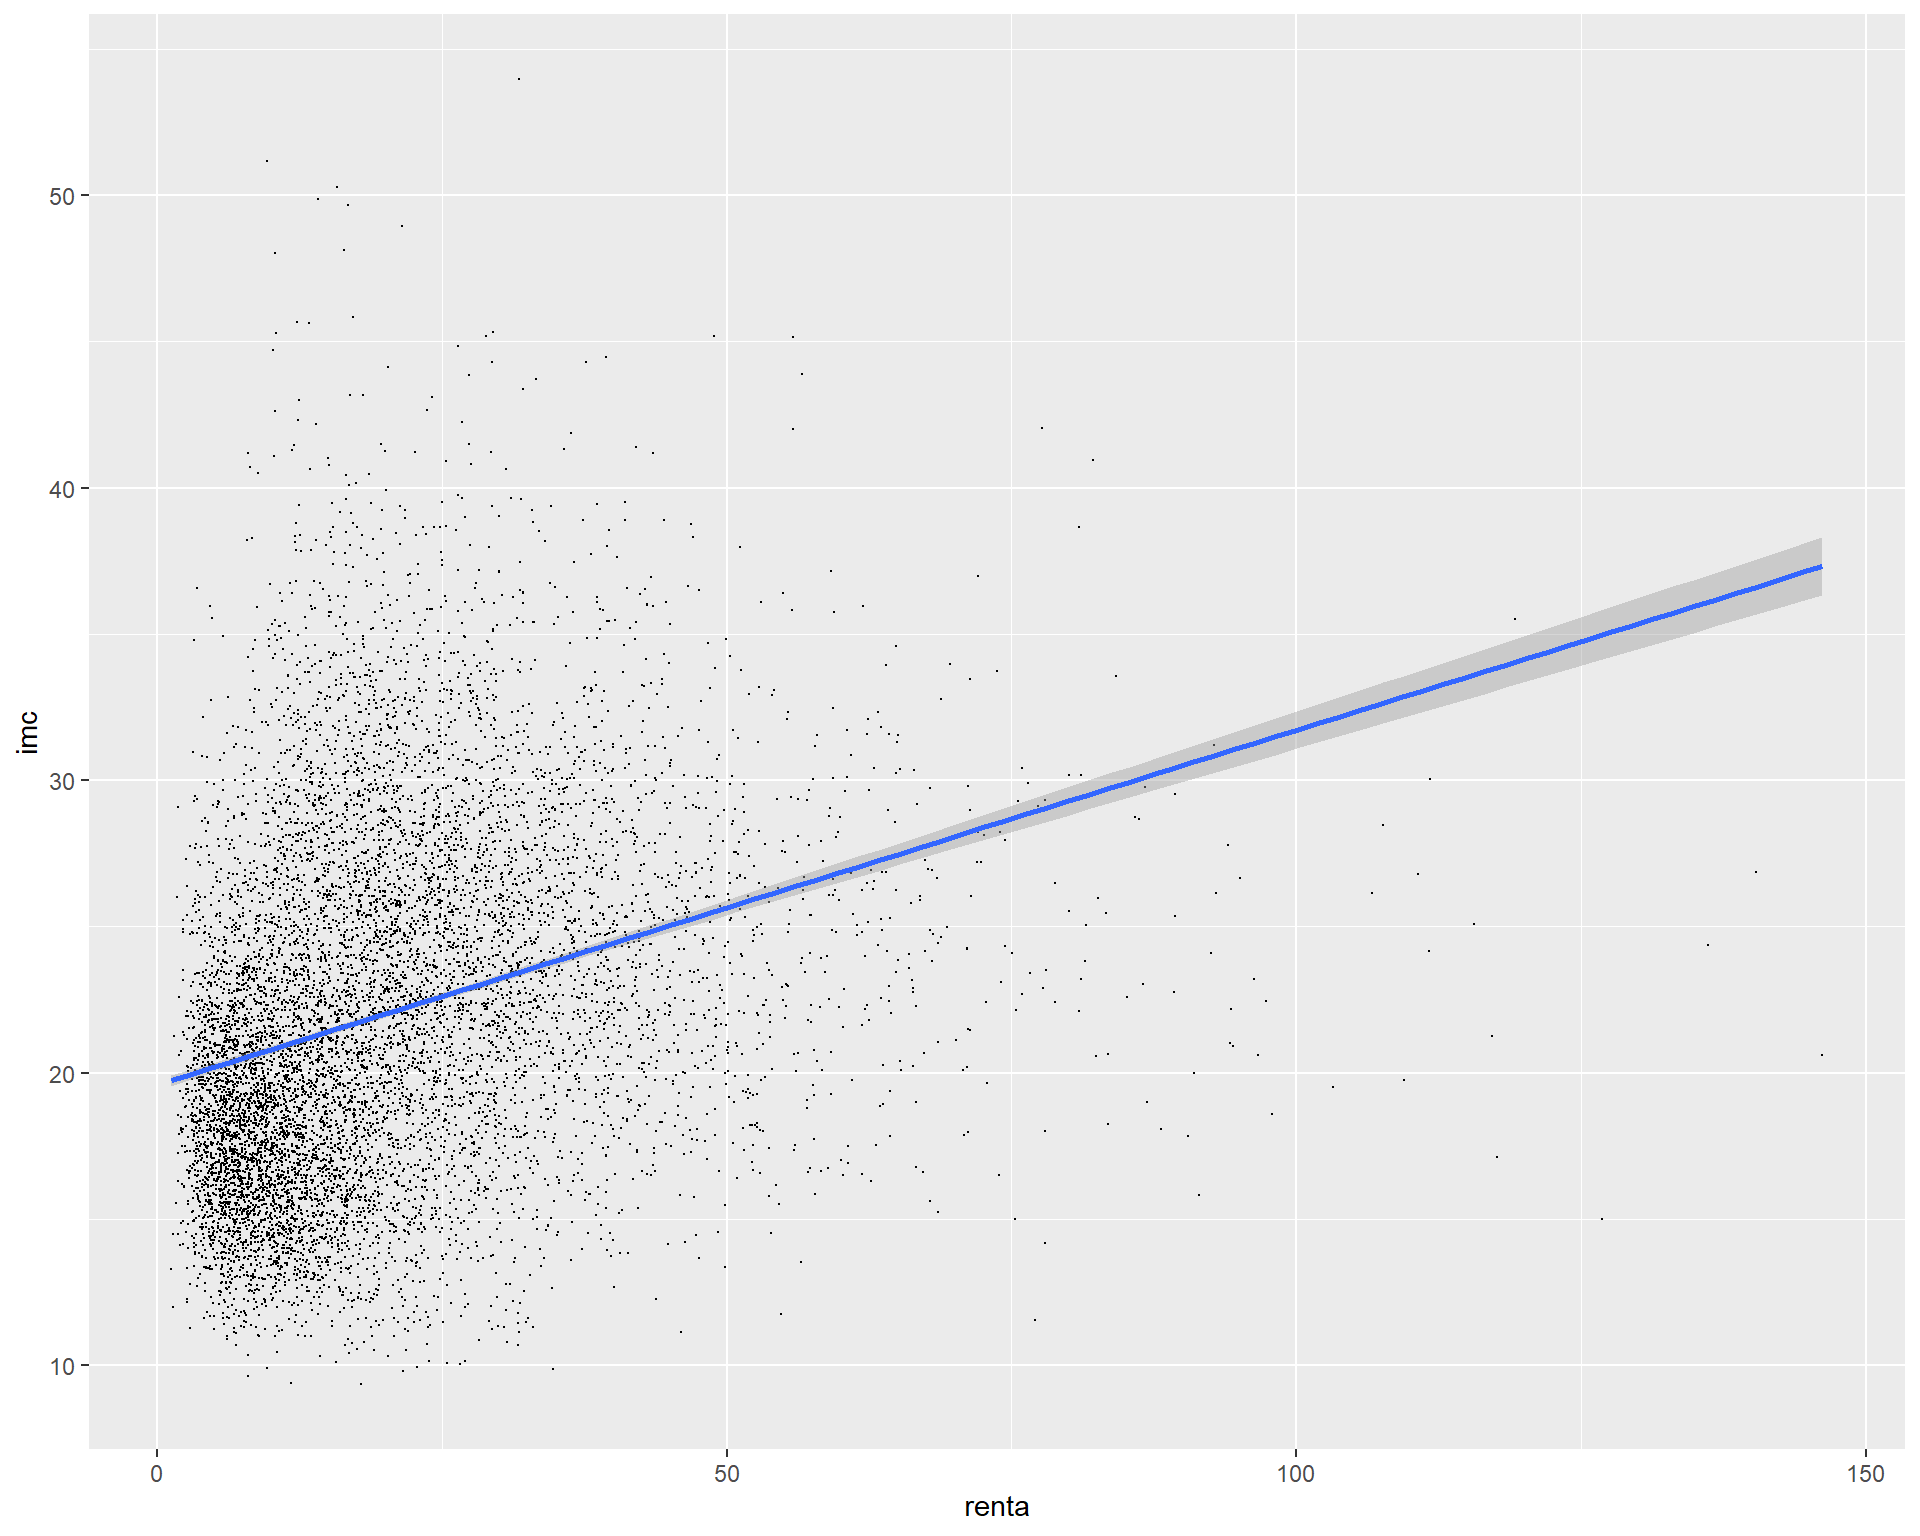
\includegraphics{graficosConR_files/figure-latex/unnamed-chunk-47-1.pdf}

\begin{Shaded}
\begin{Highlighting}[]
\NormalTok{p}\SpecialCharTok{+}\FunctionTok{scale\_x\_log10}\NormalTok{()}\SpecialCharTok{+}\FunctionTok{scale\_y\_continuous}\NormalTok{(}\AttributeTok{breaks=}\FunctionTok{seq}\NormalTok{(}\DecValTok{10}\NormalTok{,}\DecValTok{50}\NormalTok{,}\DecValTok{10}\NormalTok{),}\AttributeTok{trans=}\StringTok{"log"}\NormalTok{)}
\end{Highlighting}
\end{Shaded}

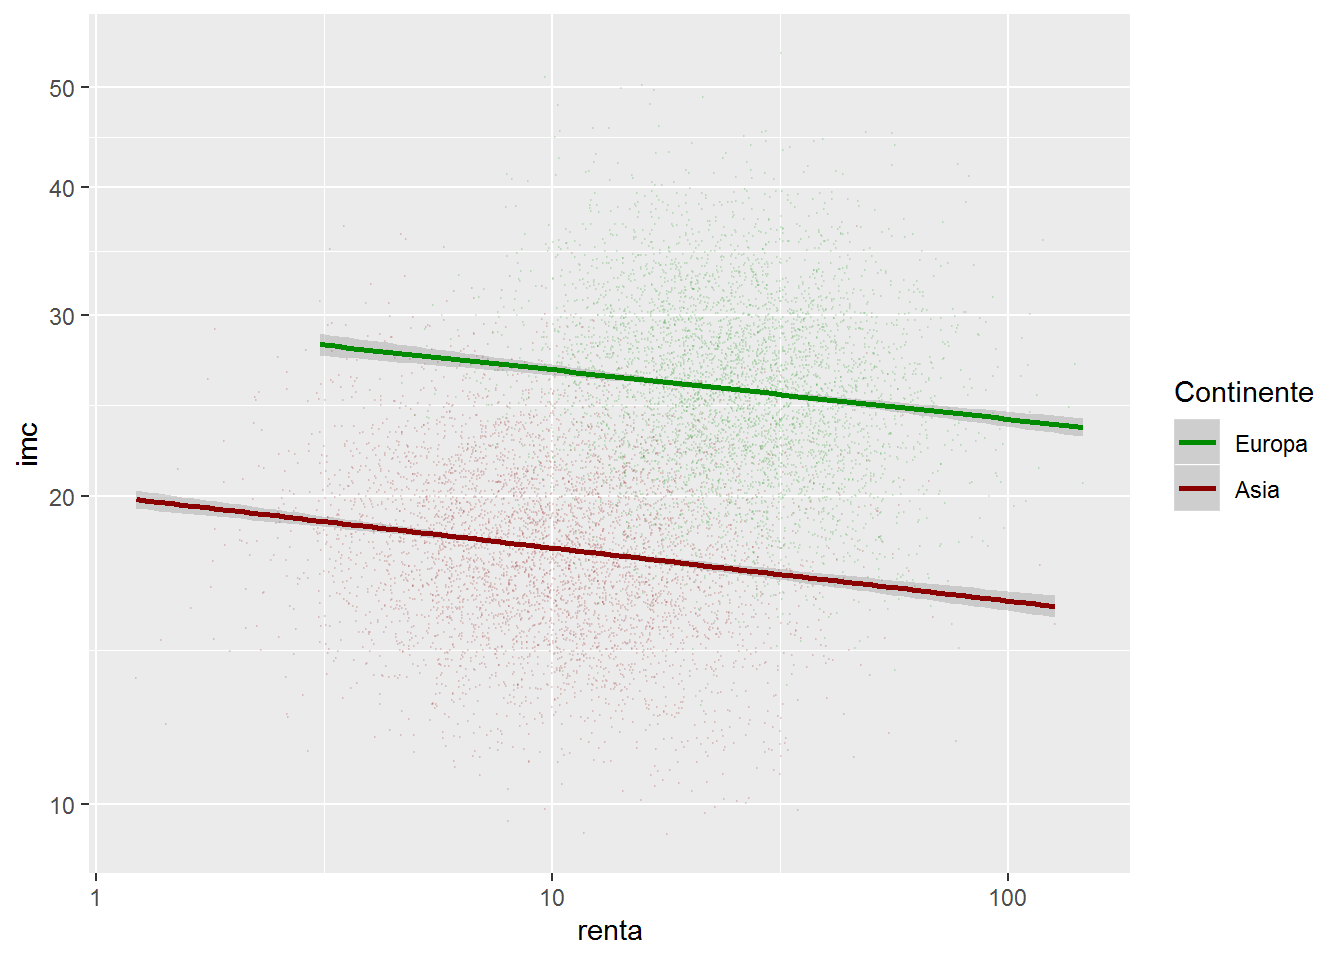
\includegraphics{graficosConR_files/figure-latex/unnamed-chunk-48-1.pdf}

\begin{Shaded}
\begin{Highlighting}[]
\FunctionTok{ggplot}\NormalTok{(obesidad,}\FunctionTok{aes}\NormalTok{(}\AttributeTok{x=}\NormalTok{renta,}\AttributeTok{y=}\NormalTok{imc,}\AttributeTok{color=}\NormalTok{region))}\SpecialCharTok{+}\FunctionTok{geom\_smooth}\NormalTok{(}\AttributeTok{method=}\StringTok{"lm"}\NormalTok{) }\SpecialCharTok{+} 
  \FunctionTok{geom\_point}\NormalTok{(}\AttributeTok{size=}\NormalTok{.}\DecValTok{1}\NormalTok{,}\AttributeTok{alpha=}\NormalTok{.}\DecValTok{1}\NormalTok{)}\SpecialCharTok{+}
  \FunctionTok{scale\_x\_log10}\NormalTok{()}\SpecialCharTok{+}\FunctionTok{scale\_y\_continuous}\NormalTok{(}\AttributeTok{breaks=}\FunctionTok{seq}\NormalTok{(}\DecValTok{10}\NormalTok{,}\DecValTok{50}\NormalTok{,}\DecValTok{10}\NormalTok{),}\AttributeTok{trans=}\StringTok{"log"}\NormalTok{)}\SpecialCharTok{+}
  \FunctionTok{scale\_color\_manual}\NormalTok{(}\StringTok{"Continente"}\NormalTok{,}\AttributeTok{values=}\FunctionTok{c}\NormalTok{(}\StringTok{"green4"}\NormalTok{,}\StringTok{"red4"}\NormalTok{),}\AttributeTok{limits=}\FunctionTok{c}\NormalTok{(}\StringTok{"Europa"}\NormalTok{,}\StringTok{"Asia"}\NormalTok{))}
\end{Highlighting}
\end{Shaded}

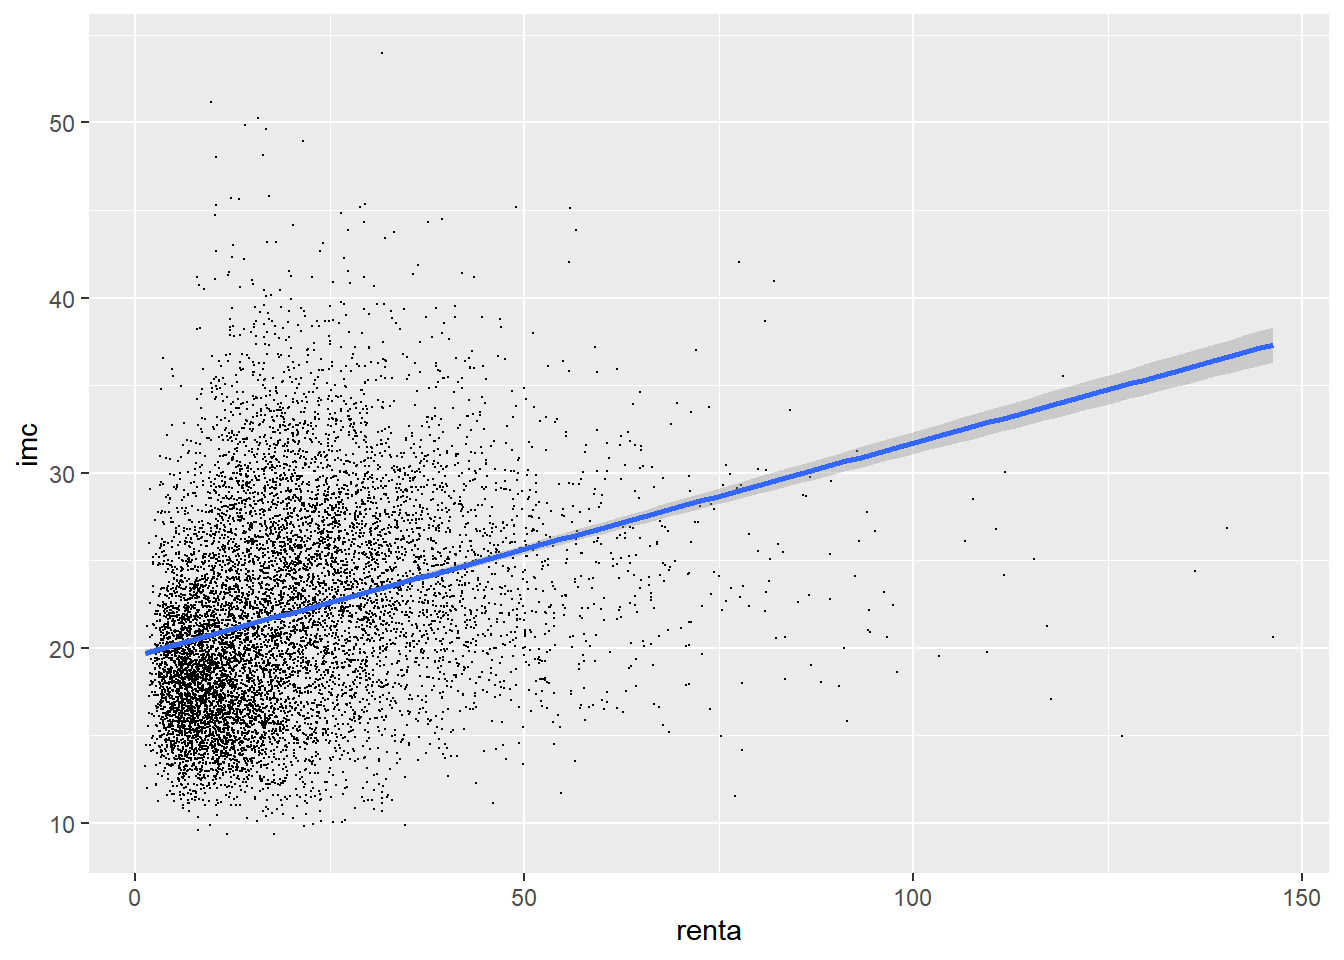
\includegraphics{graficosConR_files/figure-latex/unnamed-chunk-49-1.pdf}

\hypertarget{temas}{%
\paragraph{Temas}\label{temas}}

Los \emph{temas} de \texttt{ggplot2} permiten modificar aspectos estéticos del gráfico que no tienen que ver con los datos en sí. Eso incluye los ejes, etiquetas, colores de fondo, el tamaño de los márgenes, etc. Cambiar el tema por defecto, puede ser útil cuando los gráficos tienen que adecuarse a una imagen corporativa o atenerse a algún criterio de publicación.

El tema que usa \texttt{ggplot2} por defecto es \texttt{theme\_grey}. Al escribir \texttt{theme\_grey()} en la consola de R, se muestran alrededor de cuarenta elementos modificables y sus atributos tal y como los define dicho tema.

¿Qué se puede hacer con los temas? Una primera opción es elegir otro. Por ejemplo, se puede reemplazar el habitual por otros disponibles en el paquete como \texttt{theme\_bw} (o \texttt{theme\_classic}) haciendo

\begin{Shaded}
\begin{Highlighting}[]
\NormalTok{p }\SpecialCharTok{+} \FunctionTok{facet\_grid}\NormalTok{(}\SpecialCharTok{\textasciitilde{}}\NormalTok{region) }\SpecialCharTok{+} \FunctionTok{theme\_bw}\NormalTok{()}
\NormalTok{p }\SpecialCharTok{+} \FunctionTok{facet\_grid}\NormalTok{(}\SpecialCharTok{\textasciitilde{}}\NormalTok{region) }\SpecialCharTok{+} \FunctionTok{theme\_classic}\NormalTok{()}
\end{Highlighting}
\end{Shaded}

Es posible usar tanto los temas que incluye \texttt{ggplot2} por defecto como otros creados por la comunidad. Algunos, por ejemplo, tratan de imitar el estilo de publicaciones reconocidas como The Economist o similares. Algunos están recogidos en paquetes como, por ejemplo, \texttt{ggthemes}.

\hypertarget{exportaciuxf3n-de-los-graficos}{%
\paragraph{Exportación de los graficos}\label{exportaciuxf3n-de-los-graficos}}

Una vez creado un gráfico, es posible exportarlo en diversos formatos:

\begin{itemize}
\tightlist
\item
  Imagen tipo bitmap (\texttt{jpeg},\texttt{png},\texttt{bmp},\texttt{tiff},\ldots)
\item
  Imagen vectorial (\texttt{pdf},\texttt{svg},\ldots)
\end{itemize}

La función \texttt{ggsave} guarda en un fichero el último gráfico generado con \texttt{ggplot2}. Lo hace, además, en el formato indicado en el nombre del fichero que se quiere generar. Así,

\begin{Shaded}
\begin{Highlighting}[]
\FunctionTok{ggplot}\NormalTok{(obesidad,}\FunctionTok{aes}\NormalTok{(}\AttributeTok{x=}\NormalTok{renta,}\AttributeTok{y=}\NormalTok{imc,}\AttributeTok{color=}\NormalTok{region))}\SpecialCharTok{+}\FunctionTok{geom\_smooth}\NormalTok{(}\AttributeTok{method=}\StringTok{"lm"}\NormalTok{)}
\FunctionTok{ggsave}\NormalTok{(}\StringTok{"obesidad.pdf"}\NormalTok{)}
\CommentTok{\#ggsave("mortalidad.pdf", width = 20, height = 20, units = "cm")}
\FunctionTok{ggsave}\NormalTok{(}\StringTok{"obesidad.png"}\NormalTok{)}
\end{Highlighting}
\end{Shaded}

Si no se especifica ruta, las imágenes serán guardadas en el directorio de trabajo.

\begin{nota}
Las imágenes vectoriales tienen una resolución ``infinita'' y suelen
ocupar poca memoria. Sin embargo, no todos los editores de texto admiten
este tipo de formato.
\end{nota}

\hypertarget{unos-graficos-destacados}{%
\subsubsection{Unos graficos destacados}\label{unos-graficos-destacados}}

\hypertarget{dos-ejes}{%
\paragraph{Dos ejes}\label{dos-ejes}}

\begin{rien}
Representar en un sólo gráfico las variaciones de las tasas de
mortalidad por COVID y vacunación entre países de la UE.(ver
\texttt{?sec\_axis}).
\end{rien}

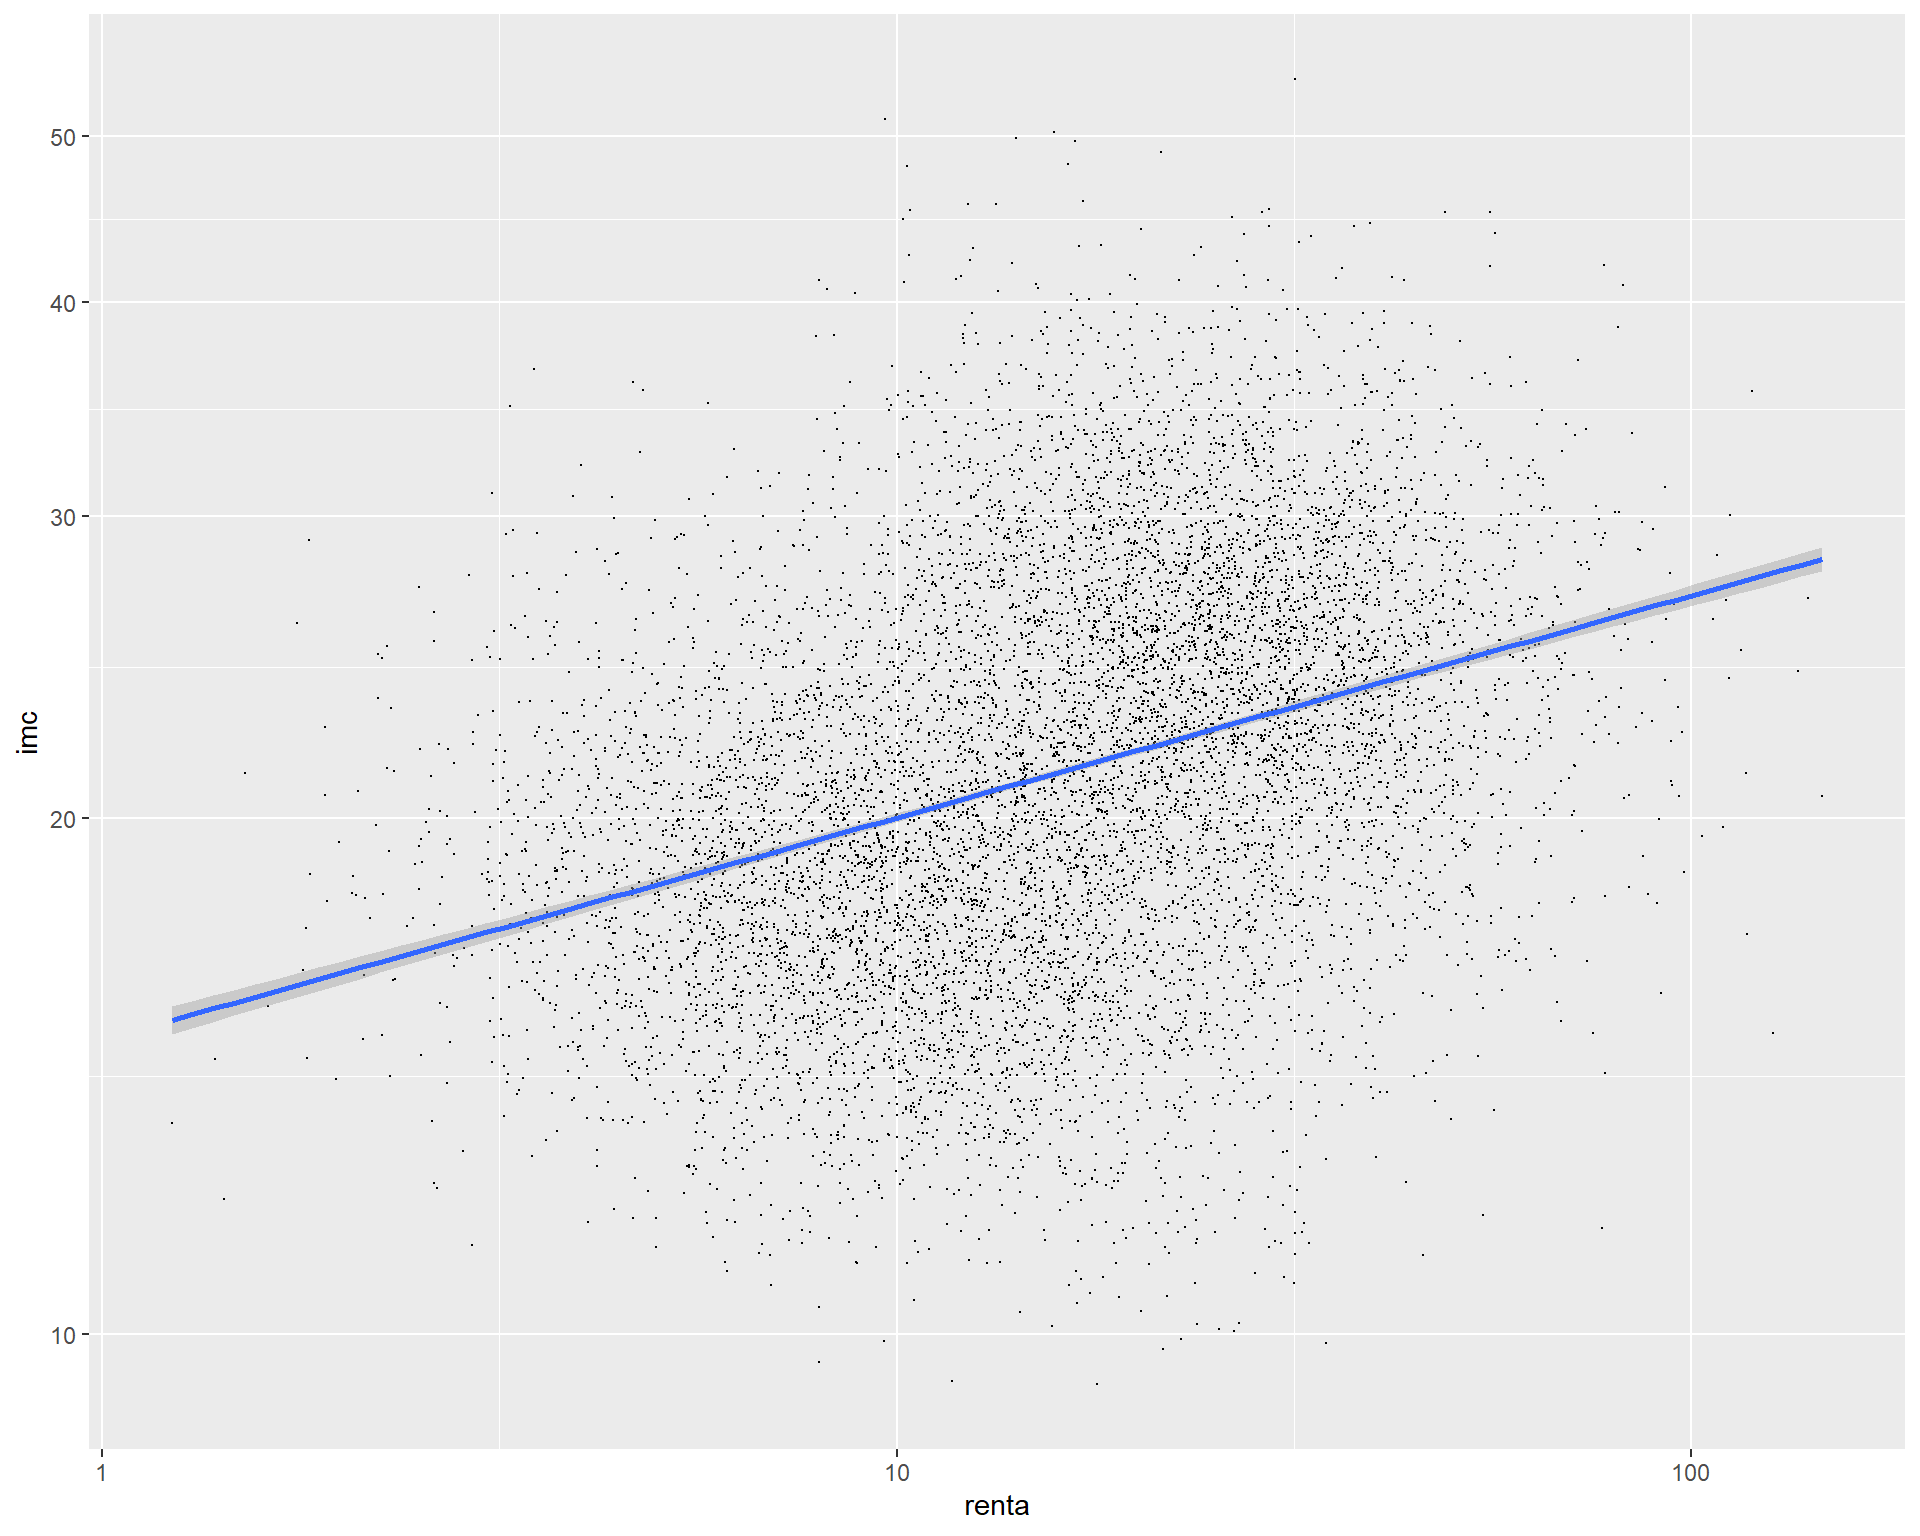
\includegraphics{graficosConR_files/figure-latex/unnamed-chunk-54-1.pdf}

\hypertarget{warming-stripes}{%
\paragraph{Warming stripes}\label{warming-stripes}}

\begin{rien}
A partir de los datos de temperaturas anuales en Lisboa de 1880 a 2008
(base de datos temp\_lisboa.csv), crear y exportar el siguiente gráfico,
utilizando la capa \texttt{geom\_tile}, el tema vacio
\texttt{theme\_void()} y la paleta de colores ``RdBu''
(\texttt{scale\_fill\_distiller(palette\ =\ \textquotesingle{}RdBu\textquotesingle{})}).
\end{rien}

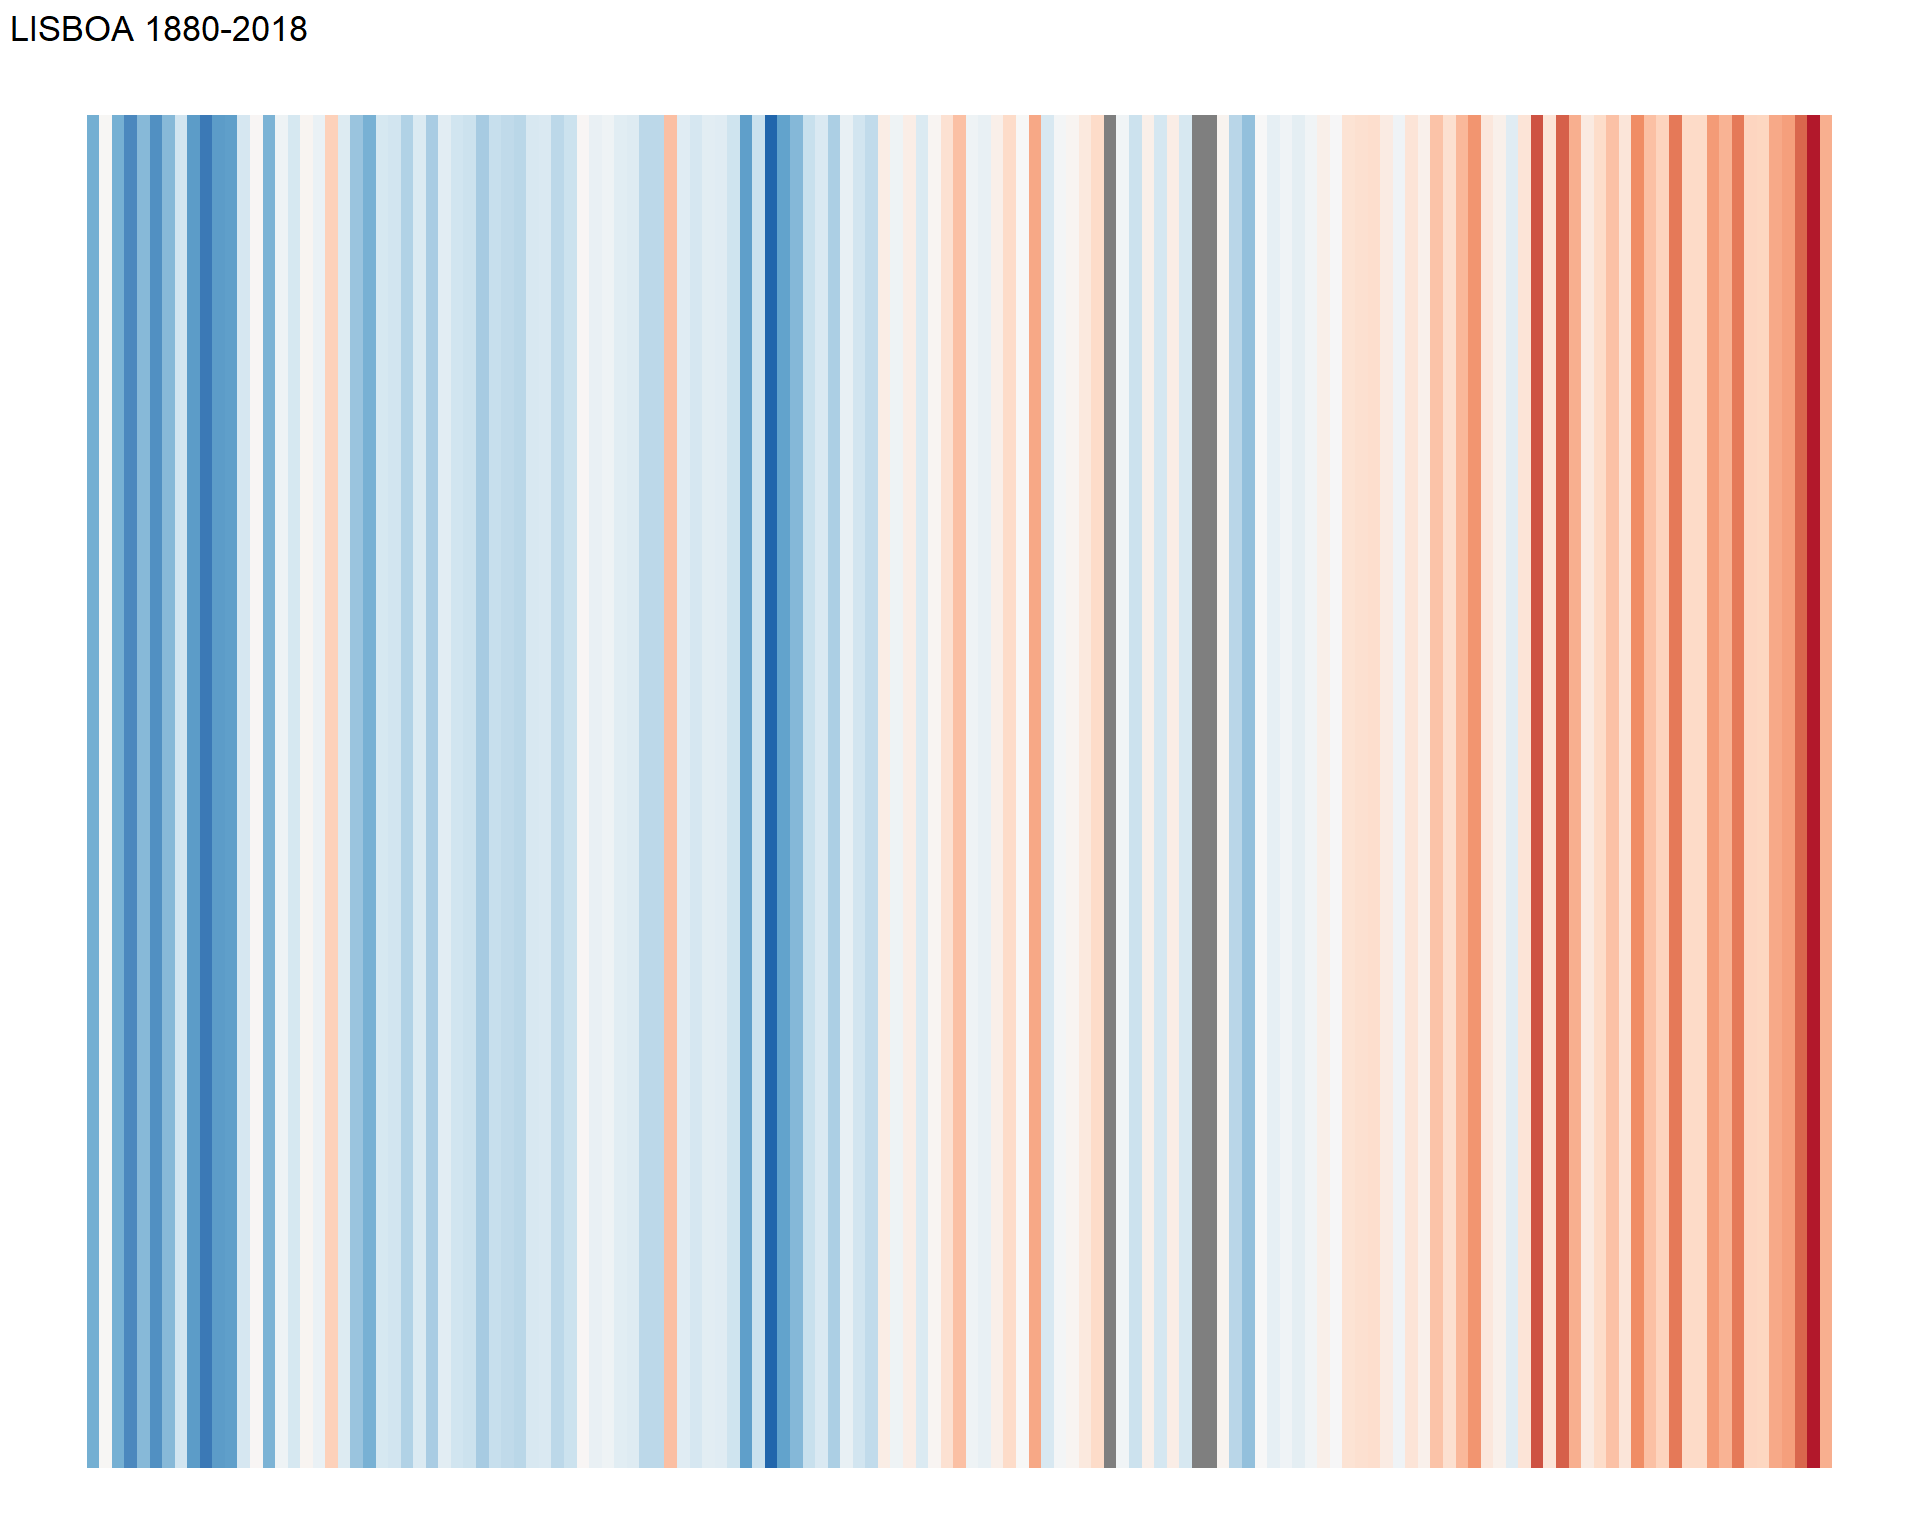
\includegraphics{graficosConR_files/figure-latex/unnamed-chunk-56-1.pdf}

\hypertarget{representaciuxf3n-por-uxe1reas}{%
\paragraph{Representación por áreas}\label{representaciuxf3n-por-uxe1reas}}

\begin{rien}
Utilizando la base de COVID, describir en un único gráfico la evolución
de esta pandemia en España de acuerdo a la edad y gravedad (se sugiere
utilizar la geometría \texttt{geom\_area}).
\end{rien}

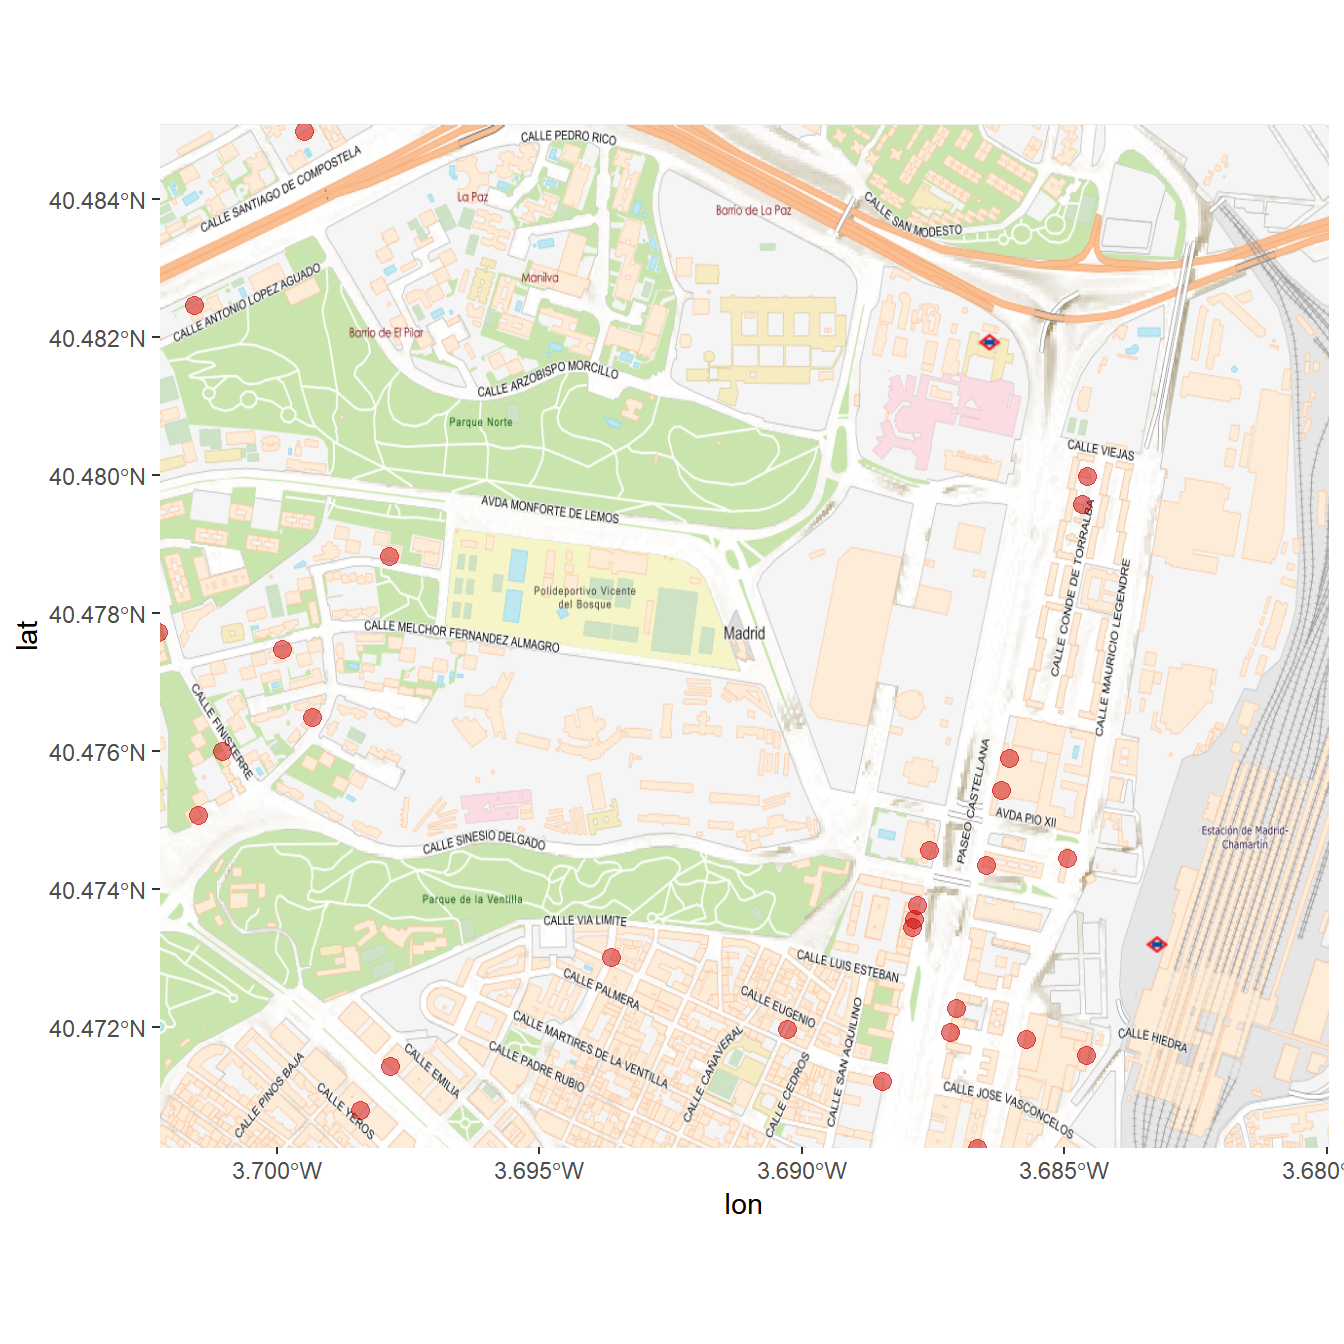
\includegraphics{graficosConR_files/figure-latex/unnamed-chunk-58-1.pdf}

\hypertarget{comparaciuxf3n-anual-de-series}{%
\paragraph{Comparación anual de series}\label{comparaciuxf3n-anual-de-series}}

\begin{ej}
Describir en un único gráfico la evolución de las defunciones en España
por año respecto a las defunciones esperadas (base de datos del MOMO).
\end{ej}

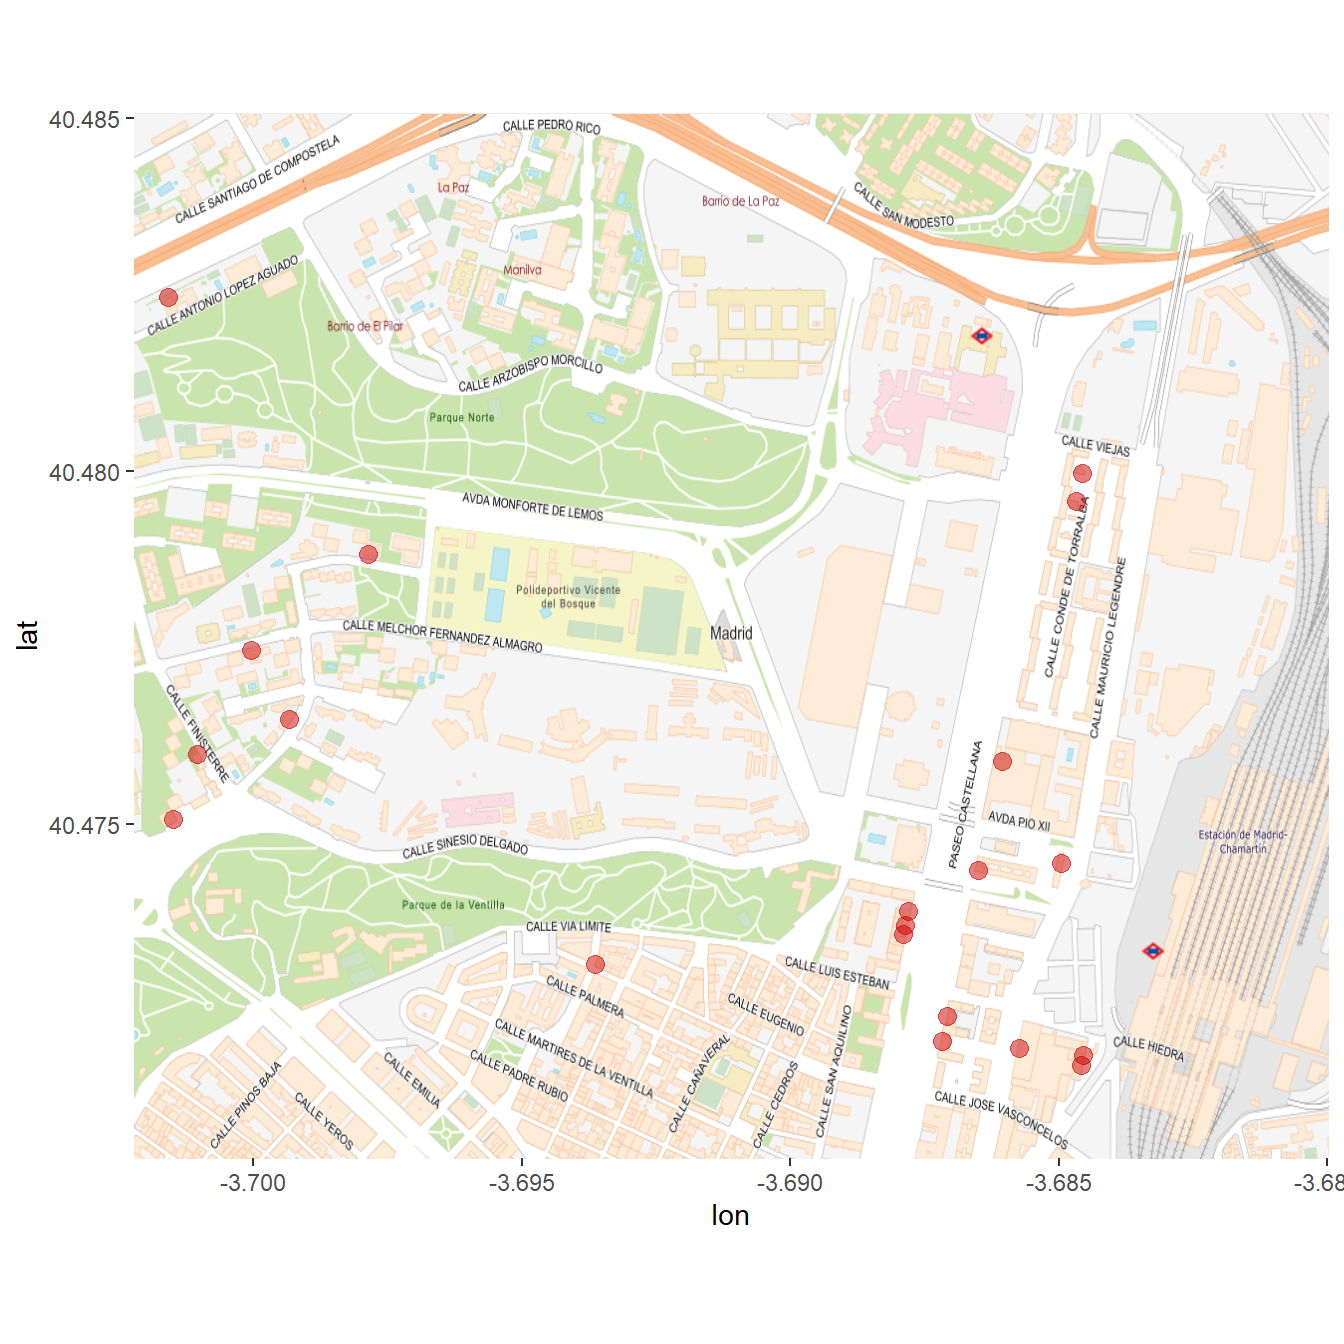
\includegraphics{graficosConR_files/figure-latex/unnamed-chunk-60-1.pdf}

\hypertarget{mapas}{%
\subsection{Mapas}\label{mapas}}

\begin{itemize}
\item
  Con \texttt{ggplot2} se puede también construir representaciones gráficas con información geográfica (puntos, segmentos, etc.): basta con que las estéticas \texttt{x} e \texttt{y} se correspondan con la longitud y la latitud de los datos.
\item
  Lo que permite hacer el paquete \texttt{ggmap} es, en esencia, añadir a una representación grafica de datos georeferenciados una capa cartográfica adicional. Para eso usa recursos disponibles en la \emph{web} a través de APIs (de Google y otros).
\end{itemize}

Un ejemplo sencillo ilustra los usos de \texttt{ggmap}. En primer lugar, se carga (si se ha instalado previamente) el paquete:

\begin{Shaded}
\begin{Highlighting}[]
\FunctionTok{library}\NormalTok{(ggmap)}
\end{Highlighting}
\end{Shaded}

Existen varios proveedores que proporcionan APIs de geolocalización. Uno de ellos es Google: dado el nombre más o menos normalizado de un lugar, la API de Google devuelve sus coordenadas. Este servicio tiene una versión gratuita que permite realizar un determinado número de consultas diarias (2500 actualmente); para usos más intensivos, es necesario adquirir una licencia.

La función \texttt{geocode} encapsula la consulta a dicha API y devuelve un objeto (un \texttt{data.frame}) que contiene las coordenadas del lugar de interés:

\begin{Shaded}
\begin{Highlighting}[]
\CommentTok{\#cne\textless{}{-} geocode(\textquotesingle{}Calle Monforte de Lemos 5, madrid\textquotesingle{}) \#sólo funciona con licencia de Google}
\NormalTok{cne }\OtherTok{\textless{}{-}}\FunctionTok{c}\NormalTok{(}\AttributeTok{lat=} \FloatTok{40.47767}\NormalTok{,}\AttributeTok{lon=}\SpecialCharTok{{-}}\FloatTok{3.691096}\NormalTok{)}

\DocumentationTok{\#\#\# Una alternativa gratuita sin limites para direcciones en España }
\CommentTok{\#require(caRtociudad)}
\CommentTok{\#cne \textless{}{-} cartociudad\_geocode(\textquotesingle{}Calle Monforte de Lemos 5, madrid\textquotesingle{})}

\DocumentationTok{\#\#\# Otra alternativa OSM}
\CommentTok{\# require(tmaptools)}
\CommentTok{\# cne=geocode\_OSM(\textquotesingle{}Monforte de Lemos 5, madrid\textquotesingle{})}
\end{Highlighting}
\end{Shaded}

La función \texttt{get\_map} consulta otro servicio de información cartográfica (GoogleMaps en el ejemplo siguiente) y descarga un mapa (que es, esencialmente, una imagen \emph{raster}).

\begin{Shaded}
\begin{Highlighting}[]
\FunctionTok{require}\NormalTok{(caRtociudad)}
\NormalTok{mapa}\OtherTok{=}\FunctionTok{cartociudad\_get\_map}\NormalTok{(cne,}\AttributeTok{radius=}\DecValTok{2}\NormalTok{)}
\CommentTok{\#cne\textless{}{-}c(left={-}3.7,bottom=40.47,right={-}3.68,top=40.485)}
\CommentTok{\#mapa \textless{}{-} get\_stamenmap(cne,zoom = 16,maptype="toner{-}lite")}
\end{Highlighting}
\end{Shaded}

Es obvio que para poder invocar las dos funciones anteriores hace falta una conexión a Internet. Sin embargo, el resto de las operaciones que se van a realizar se ejecutan localmente. Se puede, por ejemplo, representar el mapa directamente (con la función \texttt{ggmap}):

\begin{Shaded}
\begin{Highlighting}[]
\FunctionTok{ggmap}\NormalTok{(mapa)}
\end{Highlighting}
\end{Shaded}

O bien se puede marcar sobre él puntos de interés:

\begin{Shaded}
\begin{Highlighting}[]
\FunctionTok{require}\NormalTok{(data.table)}
\CommentTok{\# localización de los bares con terrazas de Madrid}
\NormalTok{terrazas}\OtherTok{=}\FunctionTok{fread}\NormalTok{(}\StringTok{"data/terrazas.csv"}\NormalTok{) }
\FunctionTok{ggmap}\NormalTok{(mapa) }\SpecialCharTok{+}  
  \FunctionTok{geom\_point}\NormalTok{(}\FunctionTok{aes}\NormalTok{(}\AttributeTok{x=}\NormalTok{lon,}\AttributeTok{y=}\NormalTok{lat),}\AttributeTok{data =}\NormalTok{ terrazas,}\AttributeTok{colour =} \StringTok{\textquotesingle{}red3\textquotesingle{}}\NormalTok{,}\AttributeTok{size =} \DecValTok{3}\NormalTok{,}\AttributeTok{alpha=}\NormalTok{.}\DecValTok{5}\NormalTok{)}
\end{Highlighting}
\end{Shaded}

\begin{center}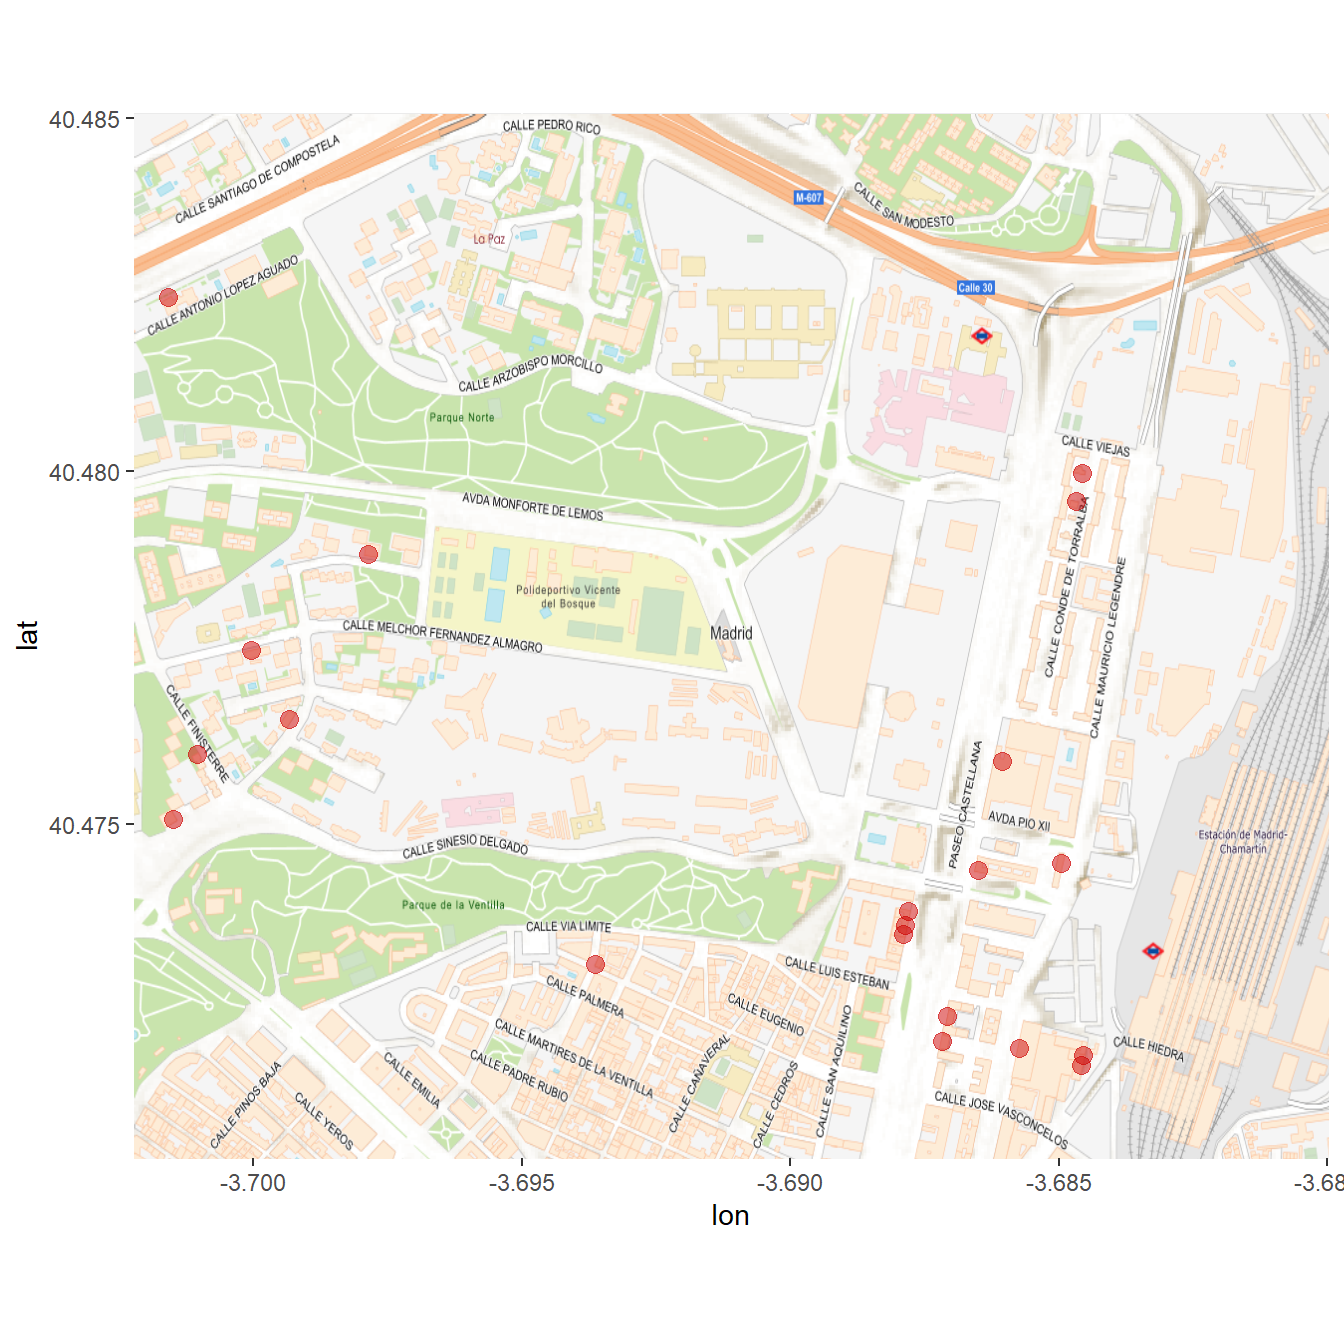
\includegraphics{graficosConR_files/figure-latex/unnamed-chunk-65-1} \end{center}

\begin{Shaded}
\begin{Highlighting}[]
\DocumentationTok{\#\#\# Obtención de la base de datos \#\#\#\#\#\#}
\NormalTok{temp}\OtherTok{=}\FunctionTok{fread}\NormalTok{(}\StringTok{\textquotesingle{}https://datos.madrid.es/egob/catalogo/200085{-}19{-}censo{-}locales.csv\textquotesingle{}}\NormalTok{,}\AttributeTok{quote=}\StringTok{\textquotesingle{}\textquotesingle{}}\NormalTok{,}\AttributeTok{dec=}\StringTok{","}\NormalTok{)}

\CommentTok{\# \#\#\#\#\#\# Cambio de proyección}
\FunctionTok{str}\NormalTok{(mapa) }\CommentTok{\#localización del lienzo}

\FunctionTok{require}\NormalTok{(sf)}
\NormalTok{Terrazas}\OtherTok{=}\FunctionTok{st\_as\_sf}\NormalTok{(temp,}\AttributeTok{coords=}\FunctionTok{c}\NormalTok{(}\StringTok{"coordenada\_x\_local"}\NormalTok{,}\StringTok{"coordenada\_y\_local"}\NormalTok{))  }\SpecialCharTok{\%\textgreater{}\%}
  \FunctionTok{st\_set\_crs}\NormalTok{(}\StringTok{"+proj=utm +zone=30"}\NormalTok{) }\SpecialCharTok{\%\textgreater{}\%}
  \FunctionTok{st\_transform}\NormalTok{(}\StringTok{"+proj=longlat"}\NormalTok{)}

\CommentTok{\# \#\#\#\#\#\# representación con sf}
\FunctionTok{ggmap}\NormalTok{(mapa)}\SpecialCharTok{+}
  \FunctionTok{geom\_sf}\NormalTok{(}\AttributeTok{data=}\NormalTok{Terrazas,}\AttributeTok{inherit.aes =} \ConstantTok{FALSE}\NormalTok{,}\AttributeTok{colour =} \StringTok{\textquotesingle{}red3\textquotesingle{}}\NormalTok{,}\AttributeTok{size =} \DecValTok{3}\NormalTok{,}\AttributeTok{alpha=}\NormalTok{.}\DecValTok{5}\NormalTok{)}

\CommentTok{\# }
\CommentTok{\# \# coordenadas en formato data.frame}
\NormalTok{terrazas}\OtherTok{=}\NormalTok{ Terrazas }\SpecialCharTok{\%\textgreater{}\%} \FunctionTok{st\_coordinates}\NormalTok{() }\SpecialCharTok{\%\textgreater{}\%} \FunctionTok{as.data.table}\NormalTok{()}
\FunctionTok{names}\NormalTok{(terrazas)}\OtherTok{\textless{}{-}}\FunctionTok{c}\NormalTok{(}\StringTok{"lon"}\NormalTok{,}\StringTok{"lat"}\NormalTok{)}


\CommentTok{\# \# Alternativa con mapa dinamico}
\FunctionTok{require}\NormalTok{(tmap)}
\FunctionTok{tmap\_mode}\NormalTok{(}\StringTok{"view"}\NormalTok{)}
\FunctionTok{tm\_shape}\NormalTok{(Terrazas) }\SpecialCharTok{+}
    \FunctionTok{tm\_dots}\NormalTok{(}\AttributeTok{col =} \StringTok{\textquotesingle{}red3\textquotesingle{}}\NormalTok{,}\AttributeTok{alpha=}\NormalTok{.}\DecValTok{5}\NormalTok{)}\SpecialCharTok{+}
    \FunctionTok{tm\_view}\NormalTok{(}\AttributeTok{set.view =} \FunctionTok{c}\NormalTok{(}\SpecialCharTok{{-}}\FloatTok{3.7}\NormalTok{, }\FloatTok{40.5}\NormalTok{, }\DecValTok{10}\NormalTok{)) }\CommentTok{\#cerca cne}
\end{Highlighting}
\end{Shaded}

\begin{verbatim}
\end{verbatim}

Como puede apreciarse, la sintaxis es similar a la de \texttt{ggplot2}. Una diferencia notable es que, ahora, los datos se pasan en la capa, es decir, en este caso, en la función \texttt{geom\_point}.

\hypertarget{muxe1s-ejemplos-de-mapas-con-puntos}{%
\subsubsection{Más ejemplos de mapas con puntos}\label{muxe1s-ejemplos-de-mapas-con-puntos}}

En los ejemplos que siguen se va a utilizar el conjunto de datos \texttt{crimes} que forma parte del paquete \texttt{ggmap} y que incluye información geo-localizada de crímenes cometidos en la ciudad de Houston. En realidad, solo consideraremos los crímenes \emph{serios}, es decir,

\begin{Shaded}
\begin{Highlighting}[]
\NormalTok{crimes.houston }\OtherTok{\textless{}{-}} \FunctionTok{subset}\NormalTok{(crime,}\SpecialCharTok{!}\NormalTok{crime}\SpecialCharTok{$}\NormalTok{offense }\SpecialCharTok{\%in\%} \FunctionTok{c}\NormalTok{(}\StringTok{"auto theft"}\NormalTok{, }\StringTok{"theft"}\NormalTok{, }\StringTok{"burglary"}\NormalTok{))}
\end{Highlighting}
\end{Shaded}

El tipo de mapas más simples son los que se limitan a representar puntos sobre una capa cartográfica.

\begin{Shaded}
\begin{Highlighting}[]
\CommentTok{\#require(tmaptools) \#para geolocalizar Houston}
\CommentTok{\#houston\textless{}{-}geocode\_OSM(\textquotesingle{}Houston\textquotesingle{})}
\NormalTok{houston}\OtherTok{=}\FunctionTok{c}\NormalTok{(}\AttributeTok{left =} \SpecialCharTok{{-}}\FloatTok{95.4}\NormalTok{, }\AttributeTok{bottom =} \FloatTok{29.74}\NormalTok{, }\AttributeTok{right =} \SpecialCharTok{{-}}\FloatTok{95.35}\NormalTok{, }\AttributeTok{top =} \FloatTok{29.78}\NormalTok{) }\CommentTok{\#barrio alrededor de Lousiana Street}
\NormalTok{houston.callejero }\OtherTok{\textless{}{-}} \FunctionTok{get\_stamenmap}\NormalTok{(houston,}\AttributeTok{zoom=}\DecValTok{14}\NormalTok{,}\AttributeTok{maptype=}\StringTok{"toner{-}lite"}\NormalTok{)}

\NormalTok{p }\OtherTok{\textless{}{-}} \FunctionTok{ggmap}\NormalTok{(houston.callejero)}
\NormalTok{p }\SpecialCharTok{+} \FunctionTok{geom\_point}\NormalTok{(}\FunctionTok{aes}\NormalTok{(}\AttributeTok{x =}\NormalTok{ lon, }\AttributeTok{y =}\NormalTok{ lat, }\AttributeTok{colour =}\NormalTok{ offense), }\AttributeTok{data =}\NormalTok{ crimes.houston, }\AttributeTok{size =} \DecValTok{1}\NormalTok{)}
\end{Highlighting}
\end{Shaded}

\begin{center}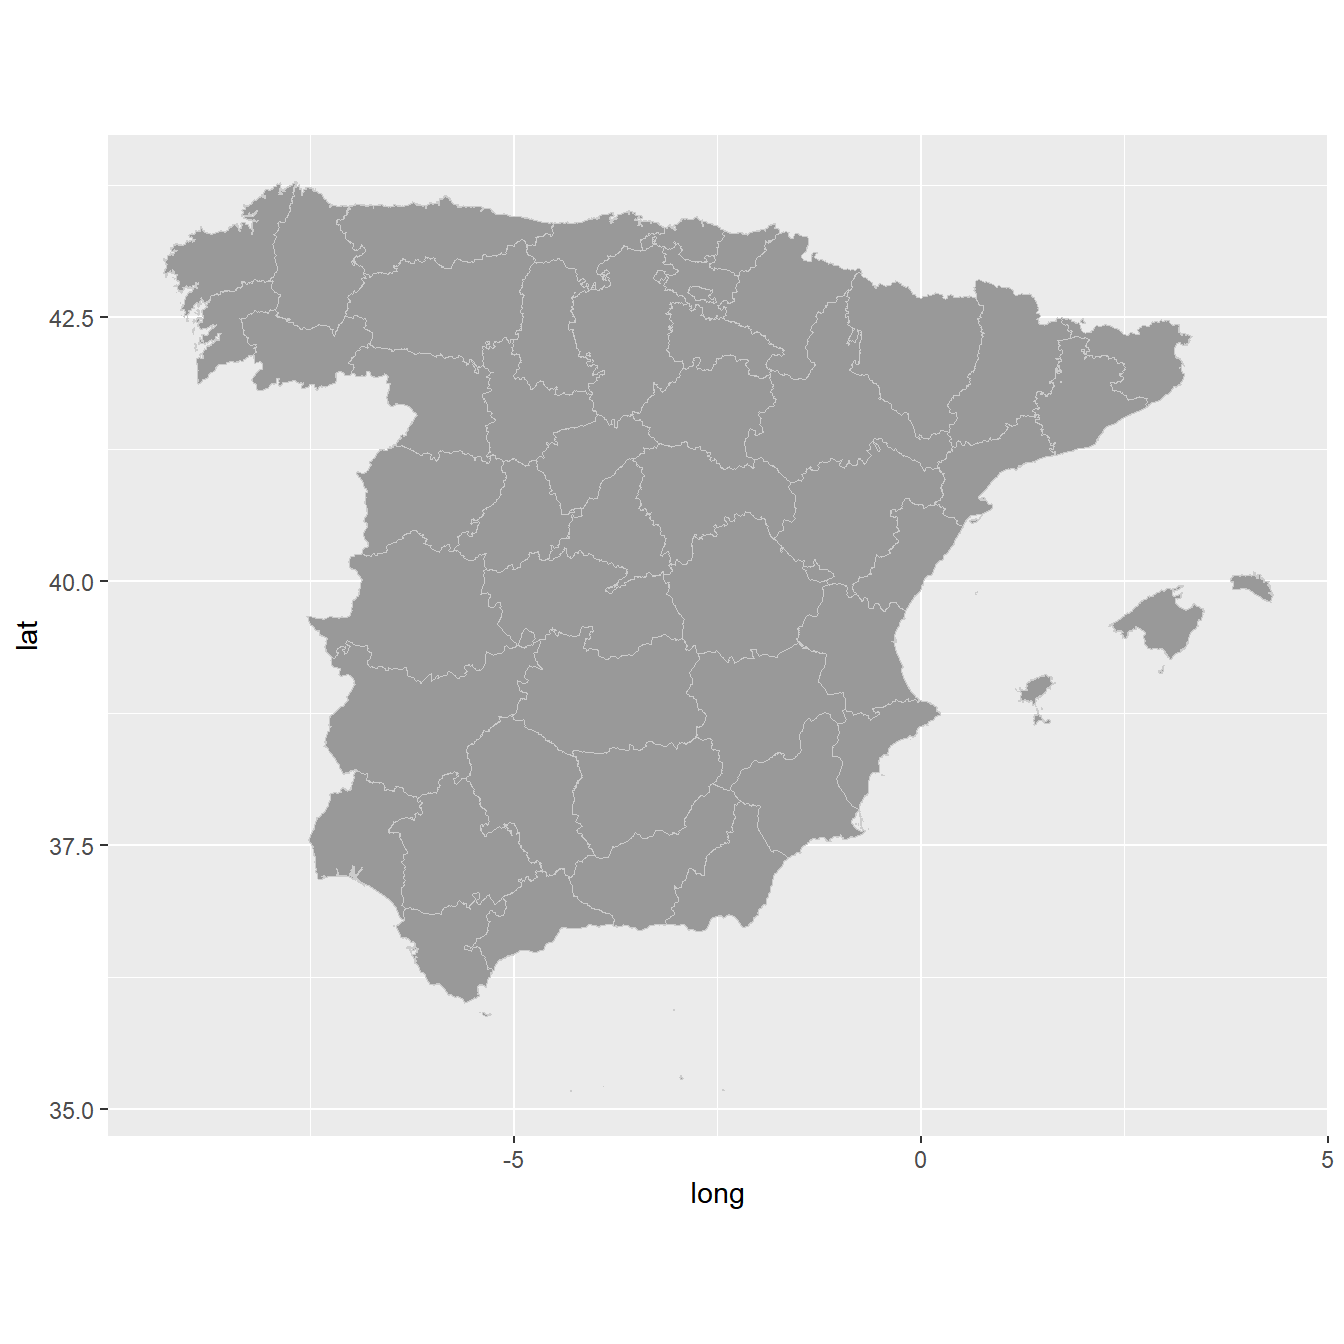
\includegraphics{graficosConR_files/figure-latex/unnamed-chunk-67-1} \end{center}

\begin{ej}
Los mecanismos conocidos de \texttt{ggplot2}, como las facetas, están
disponibles en \texttt{ggmap}. Descomponer el anterior gráfico
utilizando \texttt{facet\_wrap} por tipo de crimen (ver gráfico
siguiente). Hacer lo mismo con el día de la semana.
\end{ej}

\begin{center}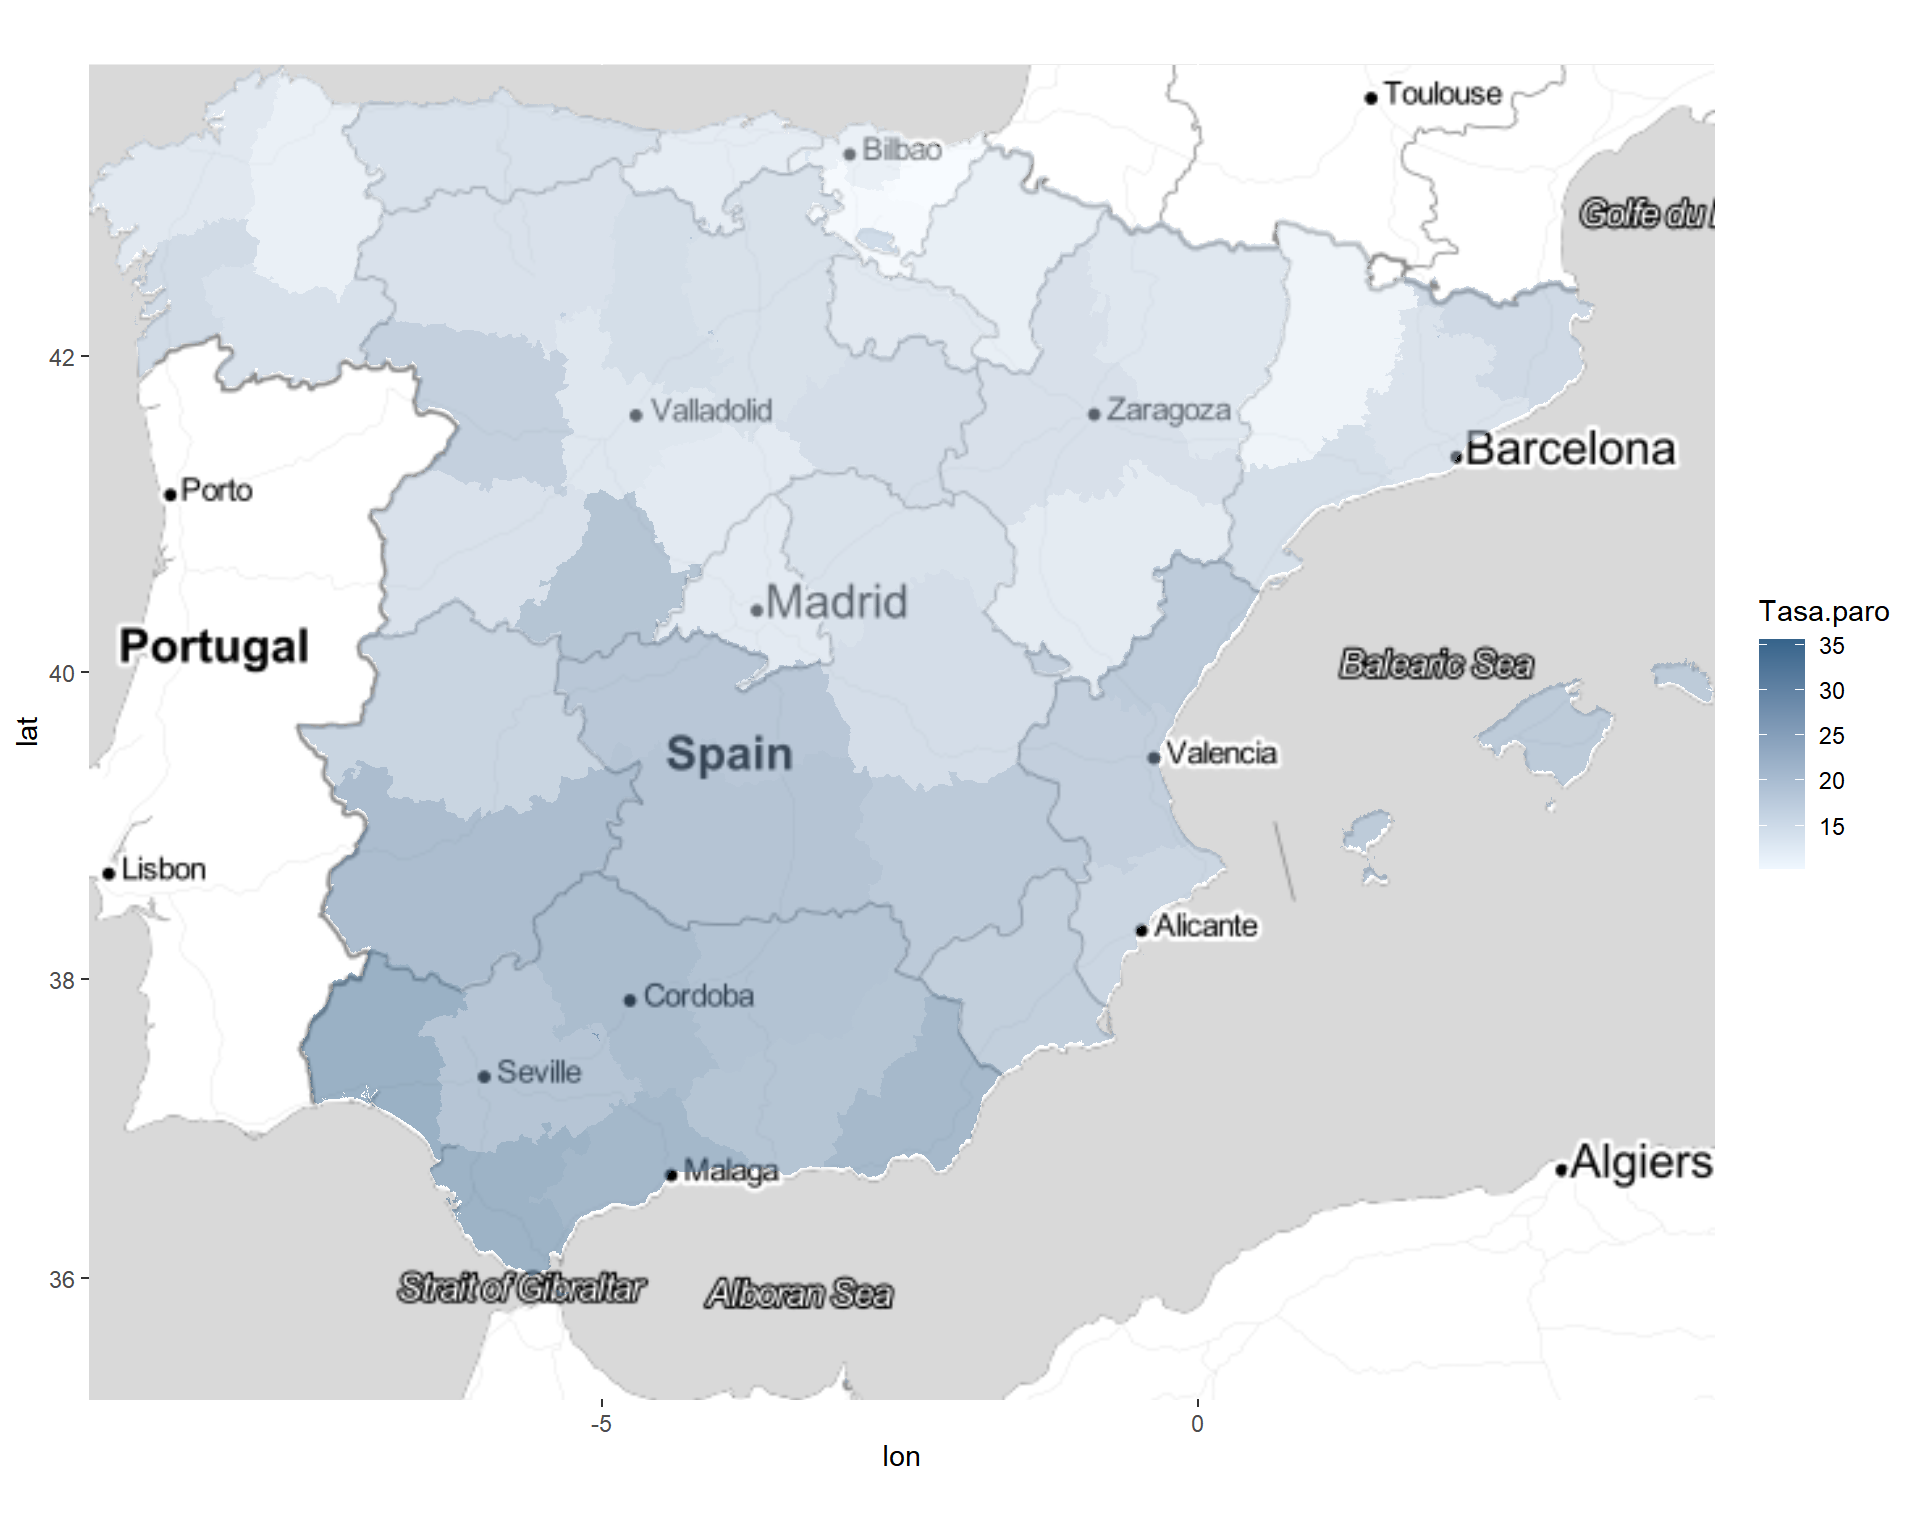
\includegraphics{graficosConR_files/figure-latex/unnamed-chunk-69-1} \end{center}

\begin{ej}
Pintar las gasolineras en el mapa de España (o de una provincia o un
municipio) utilizando el fichero \texttt{data/carburantes.csv}.
Modificar el tamaño (o color) de los puntos en función de, por ejemplo,
el precio de los carburantes.
\end{ej}

\hypertarget{muxe1s-alluxe1-de-los-puntos-densidades-y-poligonos}{%
\subsubsection{Más allá de los puntos: densidades y poligonos}\label{muxe1s-alluxe1-de-los-puntos-densidades-y-poligonos}}

Además de \texttt{geom\_point}, también están disponibles otros tipos de capas de \texttt{ggplot2}, como \texttt{stat\_bin2d}, que cuenta el número de eventos (aquí atracos) que suceden en regiones cuadradas de un tamaño predefinido. Se puede también utilizar \texttt{stat\_density2d}, que representa densidades, para identificar las zonas de mayor criminalidad.

\begin{Shaded}
\begin{Highlighting}[]
\NormalTok{p }\SpecialCharTok{+} \FunctionTok{stat\_density2d}\NormalTok{(}\FunctionTok{aes}\NormalTok{(}\AttributeTok{x =}\NormalTok{ lon, }\AttributeTok{y =}\NormalTok{ lat, }\AttributeTok{alpha =}\NormalTok{ ..level..),}\AttributeTok{fill=}\StringTok{"red4"}\NormalTok{,}
                 \AttributeTok{size =} \DecValTok{2}\NormalTok{, }\AttributeTok{data =} \FunctionTok{subset}\NormalTok{(crimes.houston,offense}\SpecialCharTok{==}\StringTok{"robbery"}\NormalTok{),}
                 \AttributeTok{geom =} \StringTok{"polygon"}\NormalTok{)}
\end{Highlighting}
\end{Shaded}

\begin{center}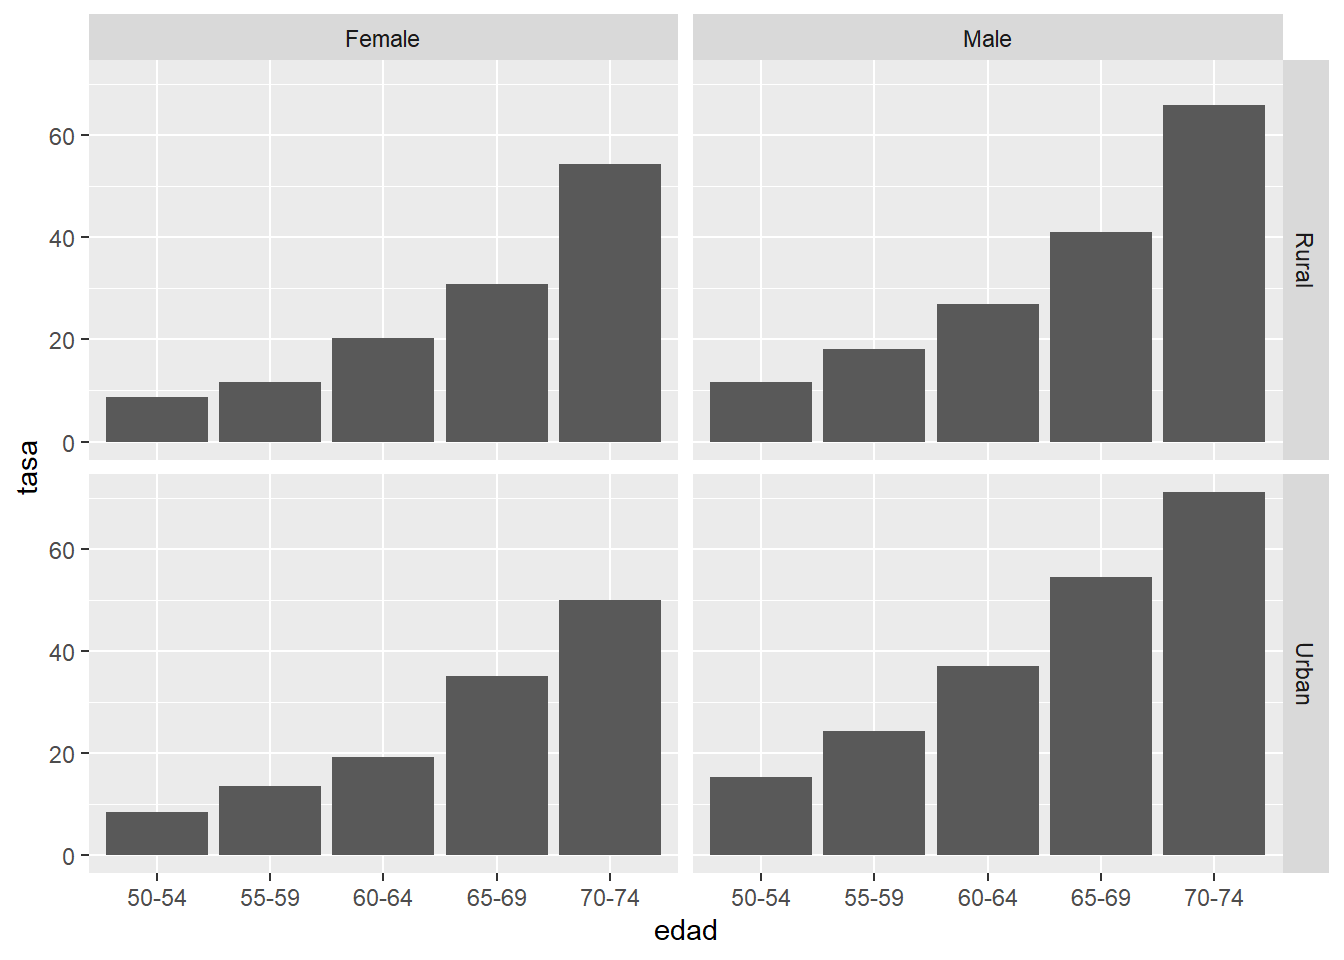
\includegraphics{graficosConR_files/figure-latex/unnamed-chunk-72-1} \end{center}

Por otra parte, la información estadística puede ser proporcionada de manera agregada en unidades espaciales (a nivel provincial, municipal, \ldots), como para los datos del paro.

Lo primero que se necesita para representar estar datos, es el conjunto de polígonos (o ``shape'') que definen las secciones geográficas. Esta información se puede por ejemplo descargar desde el servidor \texttt{GADM}mediante el paquete \texttt{raster}:

\begin{Shaded}
\begin{Highlighting}[]
\FunctionTok{require}\NormalTok{(raster)  }
\FunctionTok{require}\NormalTok{(sf)}
\NormalTok{shape }\OtherTok{\textless{}{-}} \FunctionTok{getData}\NormalTok{(}\StringTok{"GADM"}\NormalTok{, }\AttributeTok{country=} \StringTok{"Spain"}\NormalTok{, }\AttributeTok{level =} \DecValTok{2}\NormalTok{, }\AttributeTok{type=}\StringTok{"sf"}\NormalTok{) }\CommentTok{\#mapa administrativo a nivel provincial}
\NormalTok{peninsula }\OtherTok{\textless{}{-}} \FunctionTok{subset}\NormalTok{(shape,}\SpecialCharTok{!}\NormalTok{NAME\_1}\SpecialCharTok{==}\StringTok{"Islas Canarias"}\NormalTok{) }\CommentTok{\#mapa sin las islas canarias}
\NormalTok{peninsula }
\end{Highlighting}
\end{Shaded}

\begin{verbatim}
## Simple feature collection with 50 features and 13 fields
## Geometry type: MULTIPOLYGON
## Dimension:     XY
## Bounding box:  xmin: -9.301806 ymin: 35.17058 xmax: 4.328195 ymax: 43.79153
## Geodetic CRS:  WGS 84
## First 10 features:
##    GID_0 NAME_0   GID_1    NAME_1 NL_NAME_1     GID_2  NAME_2 VARNAME_2 NL_NAME_2    TYPE_2 ENGTYPE_2 CC_2   HASC_2
## 1    ESP  Spain ESP.1_1 Andalucía      <NA> ESP.1.1_1 Almería      <NA>      <NA> Provincia  Province   04 ES.AN.AM
## 2    ESP  Spain ESP.1_1 Andalucía      <NA> ESP.1.2_1   Cádiz      <NA>      <NA> Provincia  Province   11 ES.AN.CD
## 3    ESP  Spain ESP.1_1 Andalucía      <NA> ESP.1.3_1 Córdoba      <NA>      <NA> Provincia  Province   14 ES.AN.CO
## 4    ESP  Spain ESP.1_1 Andalucía      <NA> ESP.1.4_1 Granada      <NA>      <NA> Provincia  Province   18 ES.AN.GD
## 5    ESP  Spain ESP.1_1 Andalucía      <NA> ESP.1.5_1  Huelva      <NA>      <NA> Provincia  Province   21 ES.AN.HL
## 6    ESP  Spain ESP.1_1 Andalucía      <NA> ESP.1.6_1    Jaén      <NA>      <NA> Provincia  Province   23 ES.AN.JA
## 7    ESP  Spain ESP.1_1 Andalucía      <NA> ESP.1.7_1  Málaga      <NA>      <NA> Provincia  Province   29 ES.AN.MG
## 8    ESP  Spain ESP.1_1 Andalucía      <NA> ESP.1.8_1 Sevilla      <NA>      <NA> Provincia  Province   41 ES.AN.SV
## 27   ESP  Spain ESP.2_1    Aragón      <NA> ESP.2.1_1  Huesca      <NA>      <NA> Provincia  Province   22 ES.AR.HS
## 28   ESP  Spain ESP.2_1    Aragón      <NA> ESP.2.2_1  Teruel      <NA>      <NA> Provincia  Province   44 ES.AR.TE
##                          geometry
## 1  MULTIPOLYGON (((-3.030417 3...
## 2  MULTIPOLYGON (((-6.219583 3...
## 3  MULTIPOLYGON (((-5.048538 3...
## 4  MULTIPOLYGON (((-3.35014 36...
## 5  MULTIPOLYGON (((-6.836479 3...
## 6  MULTIPOLYGON (((-3.008117 3...
## 7  MULTIPOLYGON (((-4.000826 3...
## 8  MULTIPOLYGON (((-5.941178 3...
## 27 MULTIPOLYGON (((0.347473 41...
## 28 MULTIPOLYGON (((0.026484 40...
\end{verbatim}

Se puede representar este mapa utilizando \texttt{ggplot2}:

\begin{Shaded}
\begin{Highlighting}[]
\FunctionTok{ggplot}\NormalTok{(peninsula) }\SpecialCharTok{+} 
    \FunctionTok{geom\_sf}\NormalTok{(}\FunctionTok{aes}\NormalTok{(}\AttributeTok{fill=}\NormalTok{NAME\_1),}\AttributeTok{alpha=}\NormalTok{.}\DecValTok{1}\NormalTok{,}\AttributeTok{col=}\StringTok{"grey80"}\NormalTok{,}\AttributeTok{show.legend =} \ConstantTok{FALSE}\NormalTok{)}\SpecialCharTok{+}
    \FunctionTok{geom\_sf\_text}\NormalTok{(}\FunctionTok{aes}\NormalTok{(}\AttributeTok{label=}\NormalTok{NAME\_2),}\AttributeTok{size=}\DecValTok{3}\NormalTok{)}\SpecialCharTok{+}
    \FunctionTok{theme\_bw}\NormalTok{()}
\end{Highlighting}
\end{Shaded}

\begin{center}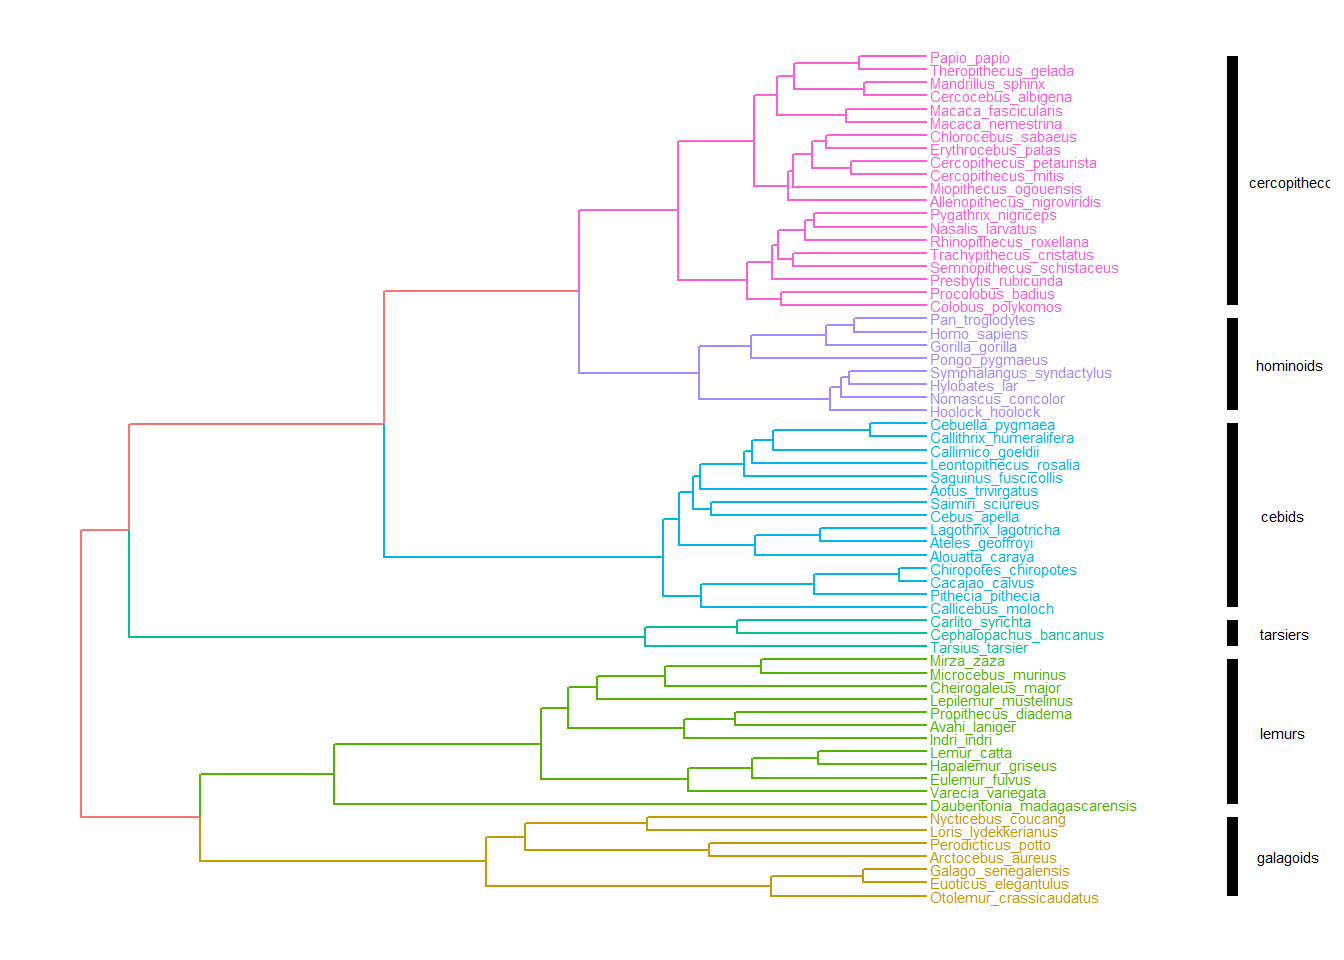
\includegraphics{graficosConR_files/figure-latex/unnamed-chunk-74-1} \end{center}

Ahora pintamos en el mapa los datos del paro (Mujeres, 2011, primer trimestre):

\begin{Shaded}
\begin{Highlighting}[]
\NormalTok{paro}\OtherTok{=}\FunctionTok{fread}\NormalTok{(}\StringTok{"data/paro.csv"}\NormalTok{,}\AttributeTok{encoding=}\StringTok{"UTF{-}8"}\NormalTok{)}
\NormalTok{paro[,id}\SpecialCharTok{:}\ErrorTok{=}\FunctionTok{sub}\NormalTok{(}\StringTok{" "}\NormalTok{,}\StringTok{"0"}\NormalTok{,}\FunctionTok{format}\NormalTok{(Prov.id,}\AttributeTok{width=}\DecValTok{2}\NormalTok{))]}
\NormalTok{Paro }\OtherTok{\textless{}{-}} \FunctionTok{subset}\NormalTok{(paro,Año}\SpecialCharTok{==}\DecValTok{2011} \SpecialCharTok{\&}\NormalTok{ Trimestre}\SpecialCharTok{==}\StringTok{"I"}\NormalTok{)}

\NormalTok{peninsula}\SpecialCharTok{$}\NormalTok{id}\OtherTok{=}\NormalTok{peninsula}\SpecialCharTok{$}\NormalTok{CC\_2}
\NormalTok{peninsula.paro}\OtherTok{=}\FunctionTok{merge}\NormalTok{(peninsula,Paro,}\AttributeTok{by=}\StringTok{"id"}\NormalTok{) }\CommentTok{\#juntamos las dos bases}

\FunctionTok{ggplot}\NormalTok{(peninsula.paro) }\SpecialCharTok{+} 
  \FunctionTok{geom\_sf}\NormalTok{(}\FunctionTok{aes}\NormalTok{(}\AttributeTok{fill=}\NormalTok{Tasa.paro), }\AttributeTok{colour =} \StringTok{"grey80"}\NormalTok{, }\AttributeTok{size =}\NormalTok{ .}\DecValTok{1}\NormalTok{) }\SpecialCharTok{+} 
  \FunctionTok{facet\_grid}\NormalTok{(}\SpecialCharTok{\textasciitilde{}}\NormalTok{ Sexo) }\SpecialCharTok{+}    
  \FunctionTok{scale\_fill\_gradient}\NormalTok{(}\StringTok{"Tasa paro"}\NormalTok{,}\AttributeTok{low=}\StringTok{"aliceblue"}\NormalTok{,}\AttributeTok{high=}\StringTok{"steelblue4"}\NormalTok{)}\SpecialCharTok{+}
  \FunctionTok{theme\_bw}\NormalTok{()}
\end{Highlighting}
\end{Shaded}

\begin{center}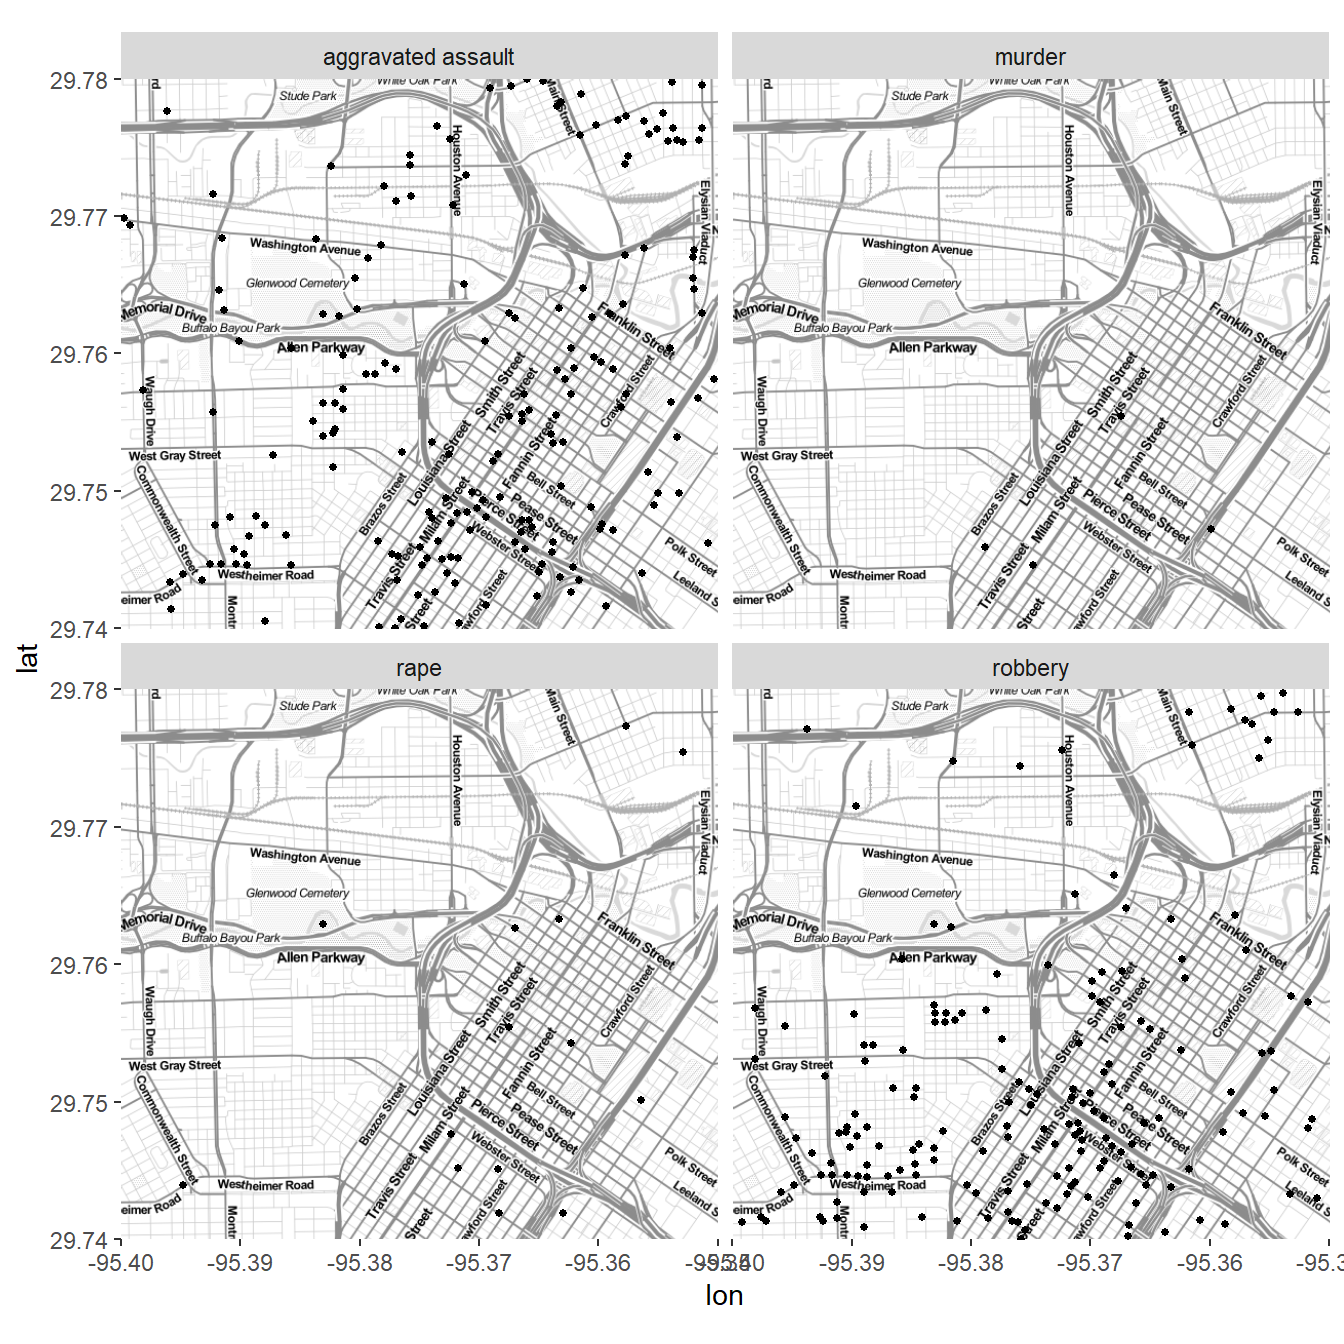
\includegraphics{graficosConR_files/figure-latex/unnamed-chunk-75-1} \end{center}

Podemos incluso dibujar este mapa, sobre un lienzo obtenido mediante \texttt{get\_map}:

\begin{Shaded}
\begin{Highlighting}[]
\NormalTok{bb}\OtherTok{=}\FunctionTok{st\_bbox}\NormalTok{(peninsula)}
\NormalTok{españa }\OtherTok{\textless{}{-}} \FunctionTok{get\_stamenmap}\NormalTok{(}\FunctionTok{unname}\NormalTok{(bb),}\AttributeTok{zoom=}\DecValTok{6}\NormalTok{,}\AttributeTok{maptype=}\StringTok{"toner{-}lite"}\NormalTok{)}

\NormalTok{mujeres}\OtherTok{=}\FunctionTok{subset}\NormalTok{(peninsula.paro,Sexo}\SpecialCharTok{==}\StringTok{"Mujeres"}\NormalTok{)}

\NormalTok{p }\OtherTok{\textless{}{-}} \FunctionTok{ggmap}\NormalTok{(españa) }\SpecialCharTok{+} 
      \FunctionTok{geom\_sf}\NormalTok{(}\AttributeTok{data =}\NormalTok{ mujeres, }\FunctionTok{aes}\NormalTok{(}\AttributeTok{fill=}\NormalTok{Tasa.paro),}\AttributeTok{alpha=}\NormalTok{.}\DecValTok{5}\NormalTok{,}\AttributeTok{inherit.aes=}\ConstantTok{FALSE}\NormalTok{) }\SpecialCharTok{+}
      \FunctionTok{scale\_fill\_distiller}\NormalTok{(}\AttributeTok{direction=}\DecValTok{1}\NormalTok{)  }

\NormalTok{p }\CommentTok{\#No muy alineado!}
\end{Highlighting}
\end{Shaded}

\begin{center}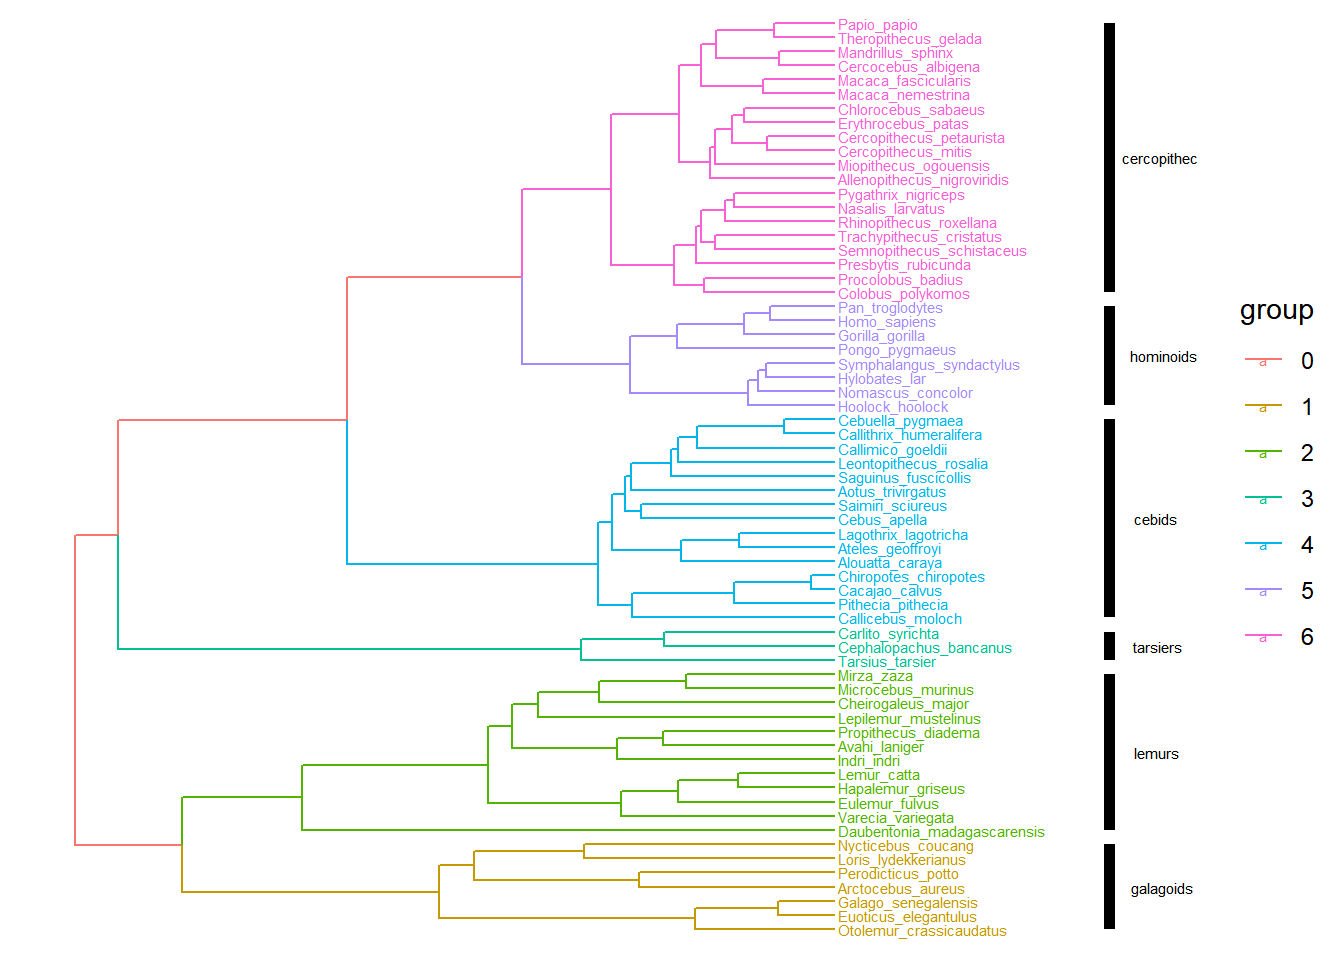
\includegraphics{graficosConR_files/figure-latex/unnamed-chunk-76-1} \end{center}

\begin{Shaded}
\begin{Highlighting}[]
\NormalTok{p }\SpecialCharTok{+}   \FunctionTok{coord\_sf}\NormalTok{(}
      \AttributeTok{crs =} \FunctionTok{st\_crs}\NormalTok{(}\DecValTok{3857}\NormalTok{), }\CommentTok{\#proyeccion del lienzo (google, osm)}
    \AttributeTok{default\_crs =} \FunctionTok{st\_crs}\NormalTok{(peninsula),  }\CommentTok{\# proyeccion de la base de datos}
\NormalTok{  ) }\CommentTok{\# ahora si}
\end{Highlighting}
\end{Shaded}

\begin{center}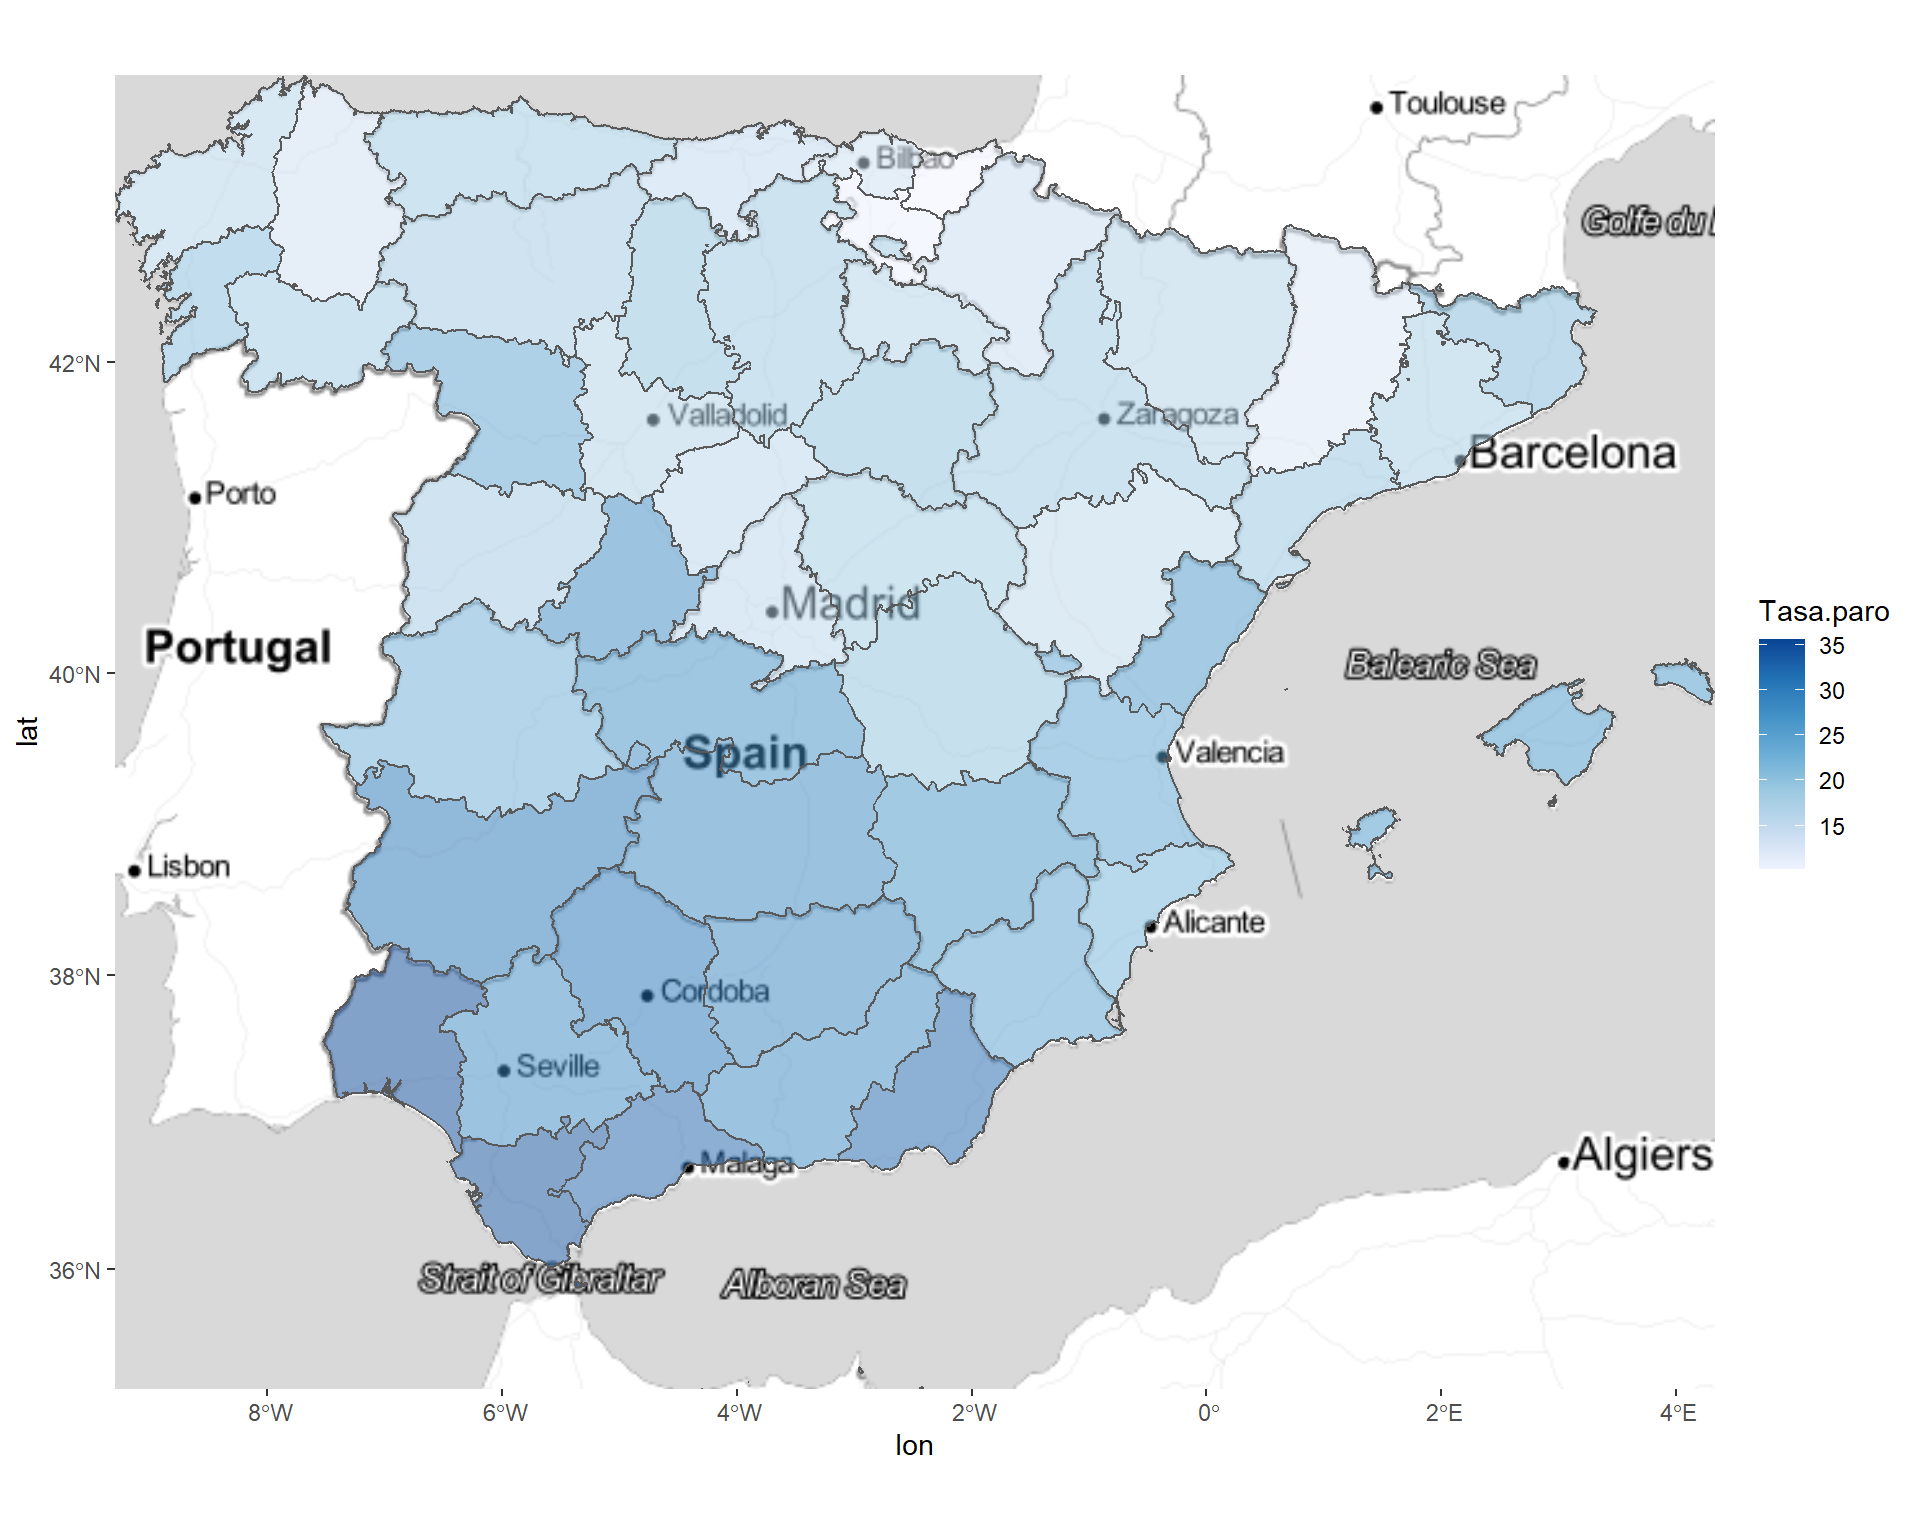
\includegraphics{graficosConR_files/figure-latex/unnamed-chunk-76-2} \end{center}

\begin{Shaded}
\begin{Highlighting}[]
\CommentTok{\#lienzo dinamico con tmap}
\CommentTok{\#tm\_shape(mujeres)+tm\_polygons("Tasa.paro")}
\end{Highlighting}
\end{Shaded}

\hypertarget{uxe1rboles-filogenuxe9ticos}{%
\subsection{Árboles filogenéticos}\label{uxe1rboles-filogenuxe9ticos}}

\hypertarget{importaciuxf3n-de-un-uxe1rbol}{%
\subsubsection{Importación de un árbol}\label{importaciuxf3n-de-un-uxe1rbol}}

\begin{itemize}
\tightlist
\item
  Un árbol filogenético es un esquema arborescente que muestra las relaciones evolutivas entre varias especies u otras entidades que se cree que tienen una ascendencia común''\,'' (Wikipedia).
\end{itemize}

\begin{figure}
\centering
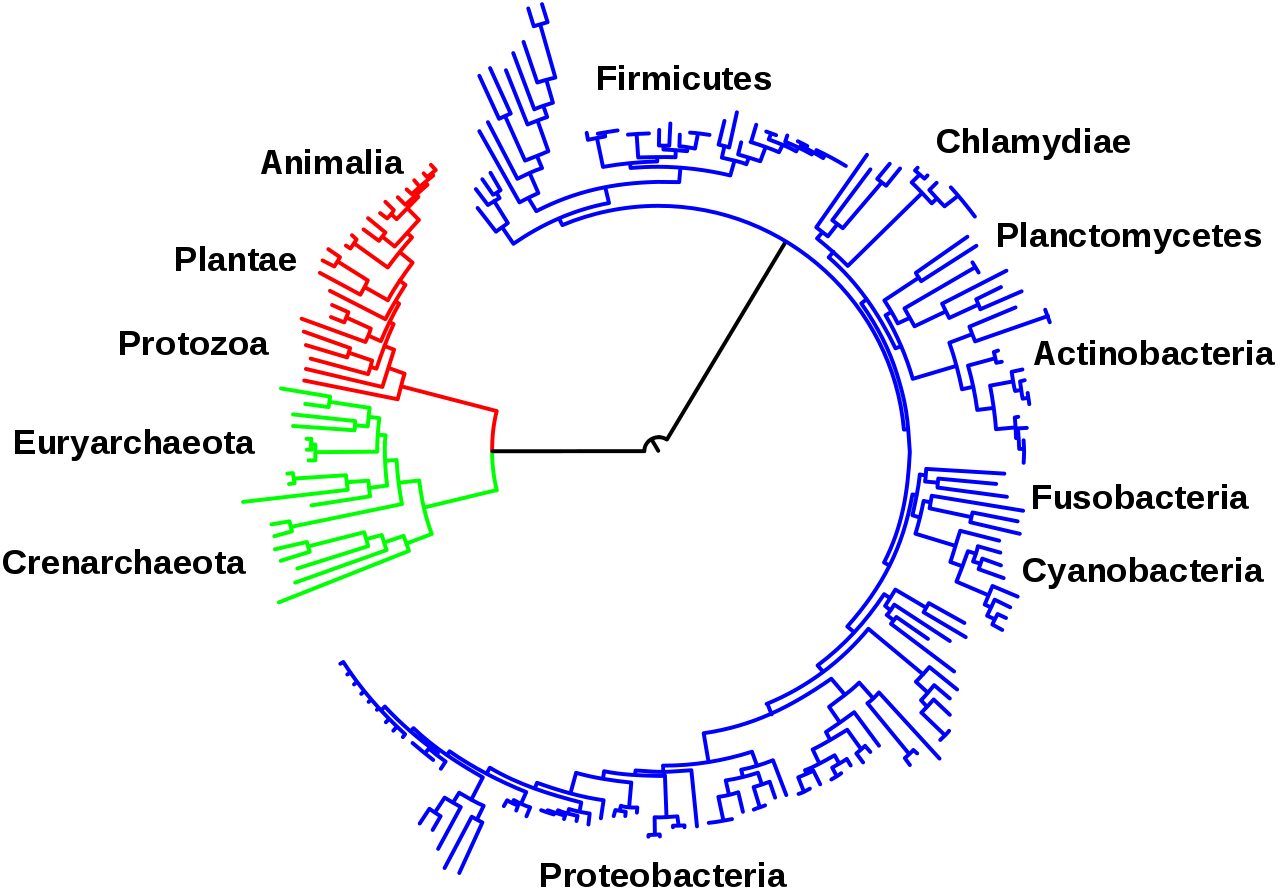
\includegraphics{imagenes/Tree_of_life_int.svg.png}
\caption{El árbol de la vida}
\end{figure}

\begin{itemize}
\item
  El método de construcción de árboles filogenéticos consiste en analizar rasgos heredables (secuencias de ADN) o caracteres morfológicos con el fin de establecer relaciones de parentesco entre especies (o taxones). Casi todos los métodos filogenéticos comienzan con una matriz de distancia en la cual las diferencias entre taxones se estiman sumando discrepancias en nucleótidos o caracteres morfológicos cuantitativos. Cada nodo del árbol representa el ancestro común.
\item
  Sin embargo, aquí no entraremos en la construcción de los arboles, sino simplemente en su representación gráfica. Suponemos pues que ya disponemos de un árbol filogenético. El paquete \texttt{treeio} sirve como interfaz para importar varios arboles en varios formatos (Newick, Nexus, NHX, jplace, \ldots.).
\end{itemize}

EL siguiente comando permite instalar el paquete \texttt{ggtree}y sus dependencias (incluye el paquete \texttt{treeio}) desde el repositorio de \texttt{Bioconductor}.

\begin{Shaded}
\begin{Highlighting}[]
\NormalTok{devtools}\SpecialCharTok{::}\FunctionTok{install\_github}\NormalTok{(}\StringTok{"YuLab{-}SMU/ggtree"}\NormalTok{)}
\end{Highlighting}
\end{Shaded}

A continuación importamos un árbol sobre filogenia de primates:

\begin{Shaded}
\begin{Highlighting}[]
\FunctionTok{require}\NormalTok{(treeio) }
\NormalTok{url}\OtherTok{=}\StringTok{"https://raw.githubusercontent.com/rgriff23/Dissertation/master/Chapter\_2/data/tree.nex"}
\NormalTok{arbol }\OtherTok{\textless{}{-}} \FunctionTok{read.nexus}\NormalTok{(url)}
\FunctionTok{summary}\NormalTok{(arbol)}
\end{Highlighting}
\end{Shaded}

\begin{verbatim}
## 
## Phylogenetic tree: arbol 
## 
##   Number of tips: 65 
##   Number of nodes: 64 
##   Branch lengths:
##     mean: 10.01834 
##     variance: 67.22004 
##     distribution summary:
##      Min.   1st Qu.    Median   3rd Qu.      Max. 
##  0.401789  4.710731  8.266731 14.271122 51.124065 
##   No root edge.
##   First ten tip labels: Allenopithecus_nigroviridis 
##                         Cercopithecus_mitis
##                         Cercopithecus_petaurista
##                         Chlorocebus_sabaeus
##                         Erythrocebus_patas
##                         Miopithecus_ogouensis
##                         Avahi_laniger
##                         Cheirogaleus_major
##                         Daubentonia_madagascarensis
##                         Eulemur_fulvus
##   No node labels.
\end{verbatim}

\hypertarget{representaciuxf3n-buxe1sica}{%
\subsubsection{Representación básica}\label{representaciuxf3n-buxe1sica}}

Vamos ahora a Explorar la estructura del árbol mediante el comando \texttt{ggtree}

\begin{Shaded}
\begin{Highlighting}[]
\FunctionTok{require}\NormalTok{(ggplot2)}
\FunctionTok{require}\NormalTok{(ggtree)}
\FunctionTok{ggtree}\NormalTok{(arbol)}
\end{Highlighting}
\end{Shaded}

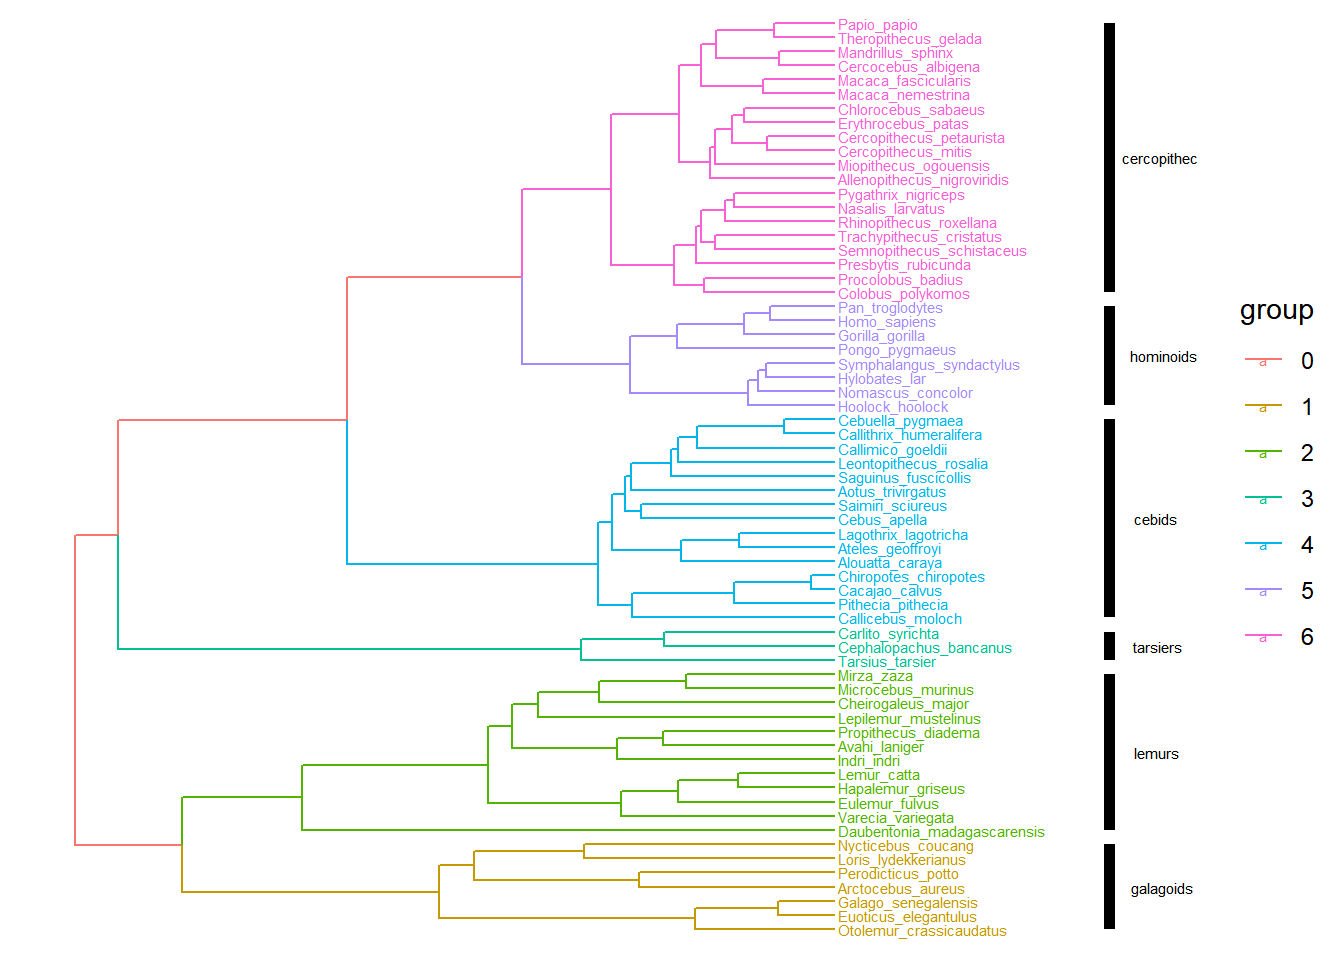
\includegraphics{graficosConR_files/figure-latex/unnamed-chunk-79-1.pdf}

Para poder añadir las etiquetas de los nodos finales utilizamos el comando \texttt{geom\_tiplab}:

\begin{Shaded}
\begin{Highlighting}[]
\FunctionTok{ggtree}\NormalTok{(arbol)}\SpecialCharTok{+}\FunctionTok{geom\_tiplab}\NormalTok{(}\AttributeTok{size=}\DecValTok{2}\NormalTok{,}\AttributeTok{offset=}\NormalTok{.}\DecValTok{5}\NormalTok{)}\SpecialCharTok{+}\FunctionTok{xlim}\NormalTok{(}\DecValTok{0}\NormalTok{,}\DecValTok{100}\NormalTok{)}
\end{Highlighting}
\end{Shaded}

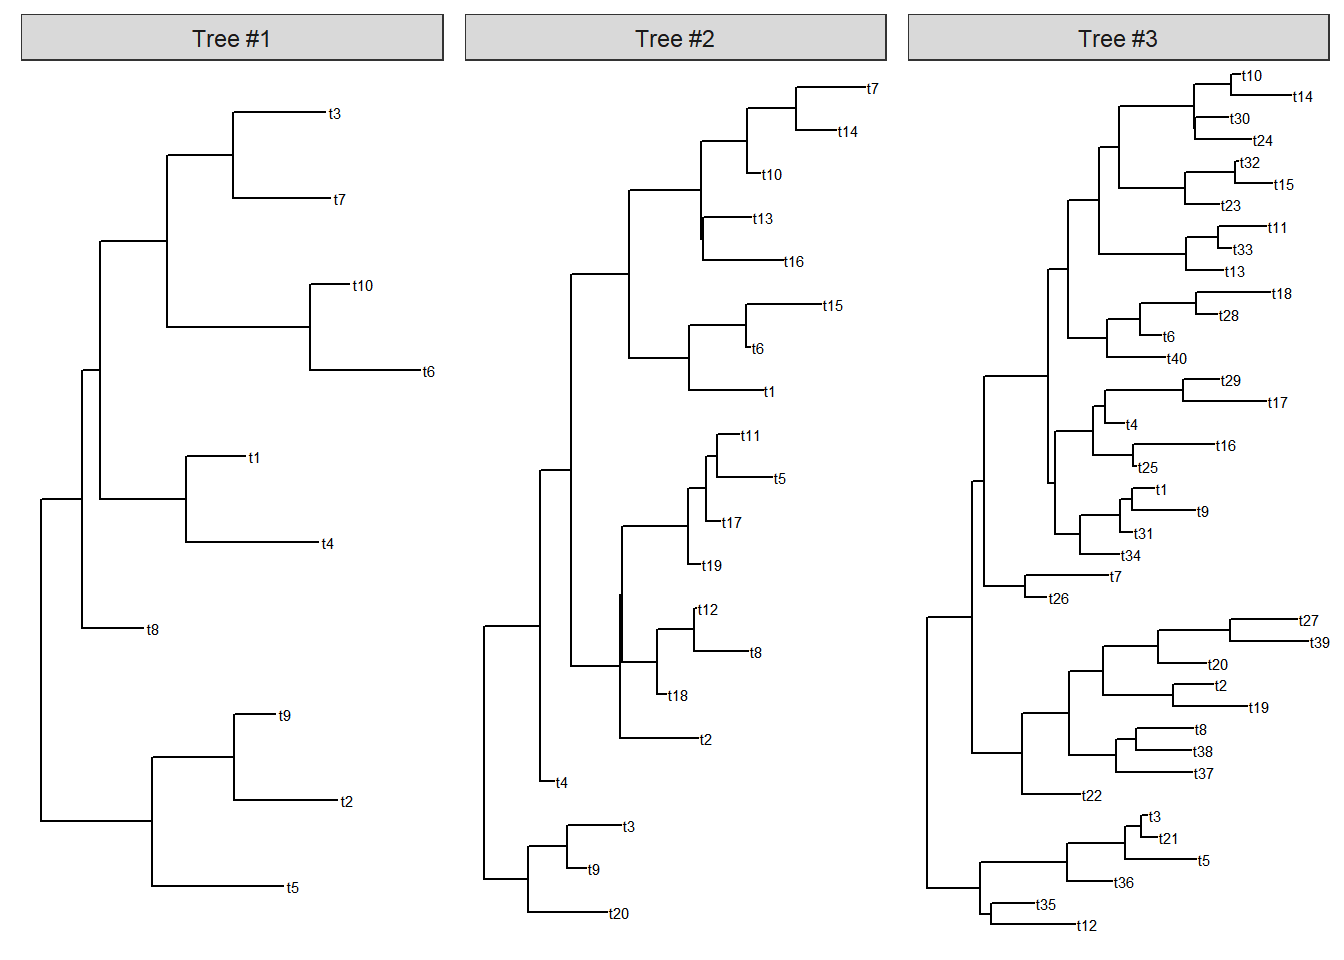
\includegraphics{graficosConR_files/figure-latex/unnamed-chunk-80-1.pdf}

Además de la representación rectangular, otros sistemas de coordenadas (circular, radial, \ldots) son disponibles utilizando la opción \texttt{layout}:

\begin{Shaded}
\begin{Highlighting}[]
\FunctionTok{require}\NormalTok{(ggplot2)}
\NormalTok{pa }\OtherTok{\textless{}{-}}\FunctionTok{ggtree}\NormalTok{(arbol) }\SpecialCharTok{+} \FunctionTok{ggtitle}\NormalTok{(}\StringTok{"rectangular"}\NormalTok{)}
\NormalTok{pa.bis }\OtherTok{\textless{}{-}} \FunctionTok{ggtree}\NormalTok{(arbol) }\SpecialCharTok{+} \FunctionTok{coord\_flip}\NormalTok{() }\SpecialCharTok{+} \FunctionTok{ggtitle}\NormalTok{(}\StringTok{"rectangular invertido"}\NormalTok{)}
\NormalTok{pb }\OtherTok{\textless{}{-}} \FunctionTok{ggtree}\NormalTok{(arbol, }\AttributeTok{layout=}\StringTok{"slanted"}\NormalTok{) }\SpecialCharTok{+} \FunctionTok{ggtitle}\NormalTok{(}\StringTok{"slanted"}\NormalTok{)}
\NormalTok{pc }\OtherTok{\textless{}{-}} \FunctionTok{ggtree}\NormalTok{(arbol, }\AttributeTok{layout=}\StringTok{"circular"}\NormalTok{) }\SpecialCharTok{+} \FunctionTok{ggtitle}\NormalTok{(}\StringTok{"circular"}\NormalTok{)}
\NormalTok{pd }\OtherTok{\textless{}{-}} \FunctionTok{ggtree}\NormalTok{(arbol, }\AttributeTok{layout=}\StringTok{"radial"}\NormalTok{) }\SpecialCharTok{+} \FunctionTok{ggtitle}\NormalTok{(}\StringTok{"radial"}\NormalTok{)}
\NormalTok{pe }\OtherTok{\textless{}{-}} \FunctionTok{ggtree}\NormalTok{(arbol, }\AttributeTok{layout=}\StringTok{"unrooted"}\NormalTok{) }\SpecialCharTok{+} \FunctionTok{ggtitle}\NormalTok{(}\StringTok{"unrooted"}\NormalTok{)}
\FunctionTok{multiplot}\NormalTok{(pa, pa.bis, pb, pc, pd, pe, }\AttributeTok{ncol=}\DecValTok{3}\NormalTok{)}
\end{Highlighting}
\end{Shaded}

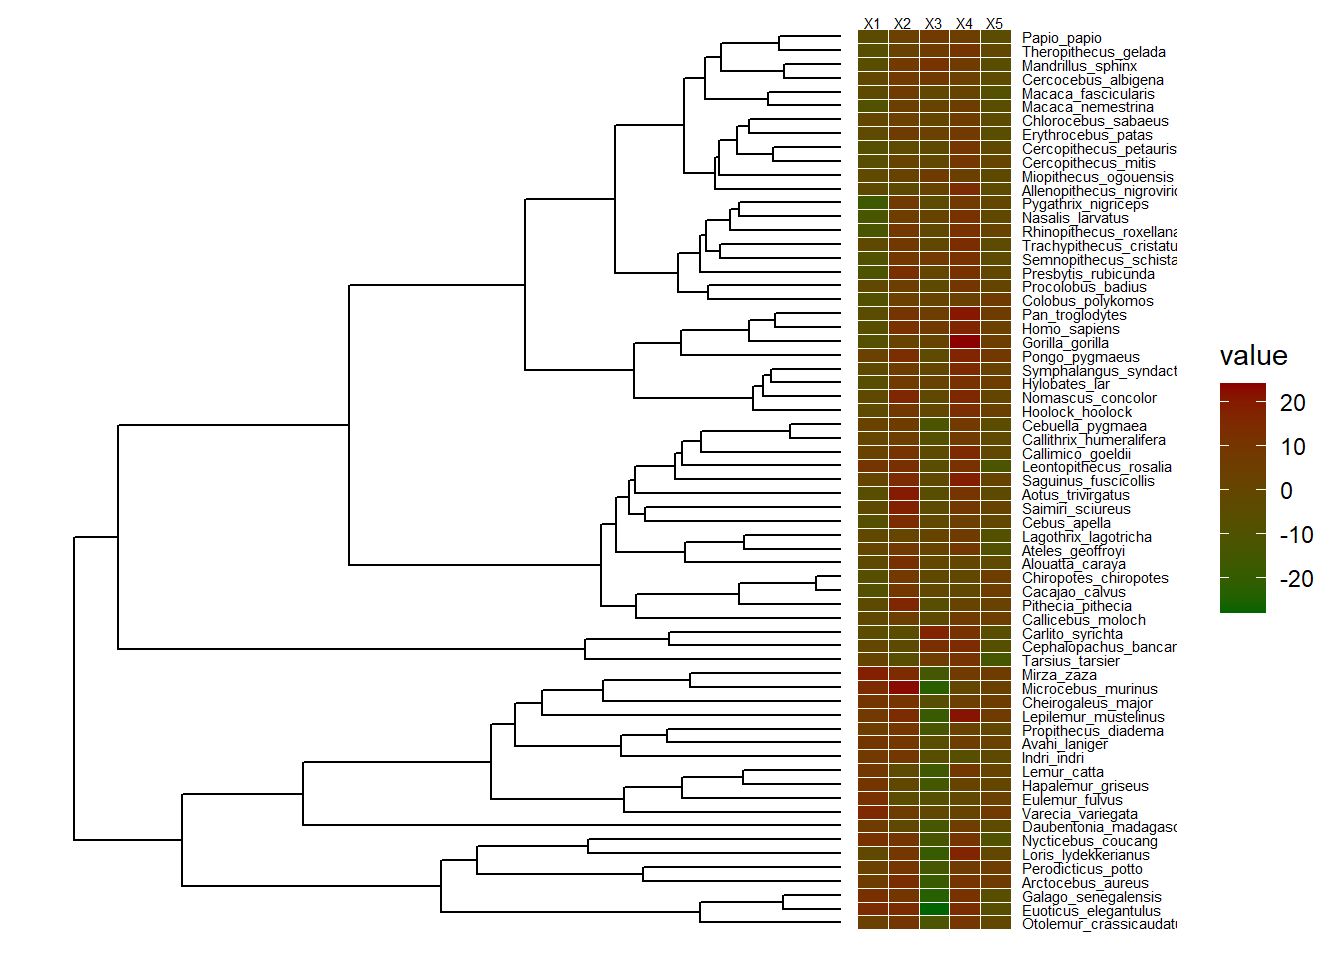
\includegraphics{graficosConR_files/figure-latex/unnamed-chunk-81-1.pdf}

\hypertarget{agrupaciuxf3n-de-nodos}{%
\subsubsection{Agrupación de nodos}\label{agrupaciuxf3n-de-nodos}}

La función \texttt{groupClade} permite agrupar nodos que comparten un mismo ancestro. A continuación agrupamos los nodos por familia de primates:
- Galagoidea (124)
- Lemuroidea (113)
- Tarsioidea (110)
- Ceboidea (96)
- Hominoidea (89)
- Cercopithecoidea (70)

\begin{Shaded}
\begin{Highlighting}[]
\NormalTok{nodos}\OtherTok{=}\FunctionTok{c}\NormalTok{(}\DecValTok{124}\NormalTok{, }\DecValTok{113}\NormalTok{, }\DecValTok{110}\NormalTok{, }\DecValTok{96}\NormalTok{, }\DecValTok{89}\NormalTok{, }\DecValTok{70}\NormalTok{)}
\NormalTok{arbol}\OtherTok{\textless{}{-}}\FunctionTok{groupClade}\NormalTok{(arbol,}\AttributeTok{.node=}\NormalTok{nodos) }\CommentTok{\#agrupación por especie}
\NormalTok{familias}\OtherTok{=}\FunctionTok{c}\NormalTok{(}\StringTok{"galagoids"}\NormalTok{,}\StringTok{"lemurs"}\NormalTok{,}\StringTok{"tarsiers"}\NormalTok{,}\StringTok{"cebids"}\NormalTok{,}\StringTok{"hominoids"}\NormalTok{,}\StringTok{"cercopithecoids"}\NormalTok{)}
\FunctionTok{ggtree}\NormalTok{(arbol, }\FunctionTok{aes}\NormalTok{(}\AttributeTok{color=}\NormalTok{group), }\AttributeTok{layout=}\StringTok{\textquotesingle{}circular\textquotesingle{}}\NormalTok{) }\SpecialCharTok{+} 
  \FunctionTok{geom\_tiplab}\NormalTok{(}\AttributeTok{size=}\DecValTok{2}\NormalTok{, }\FunctionTok{aes}\NormalTok{(}\AttributeTok{angle=}\NormalTok{angle))}
\end{Highlighting}
\end{Shaded}

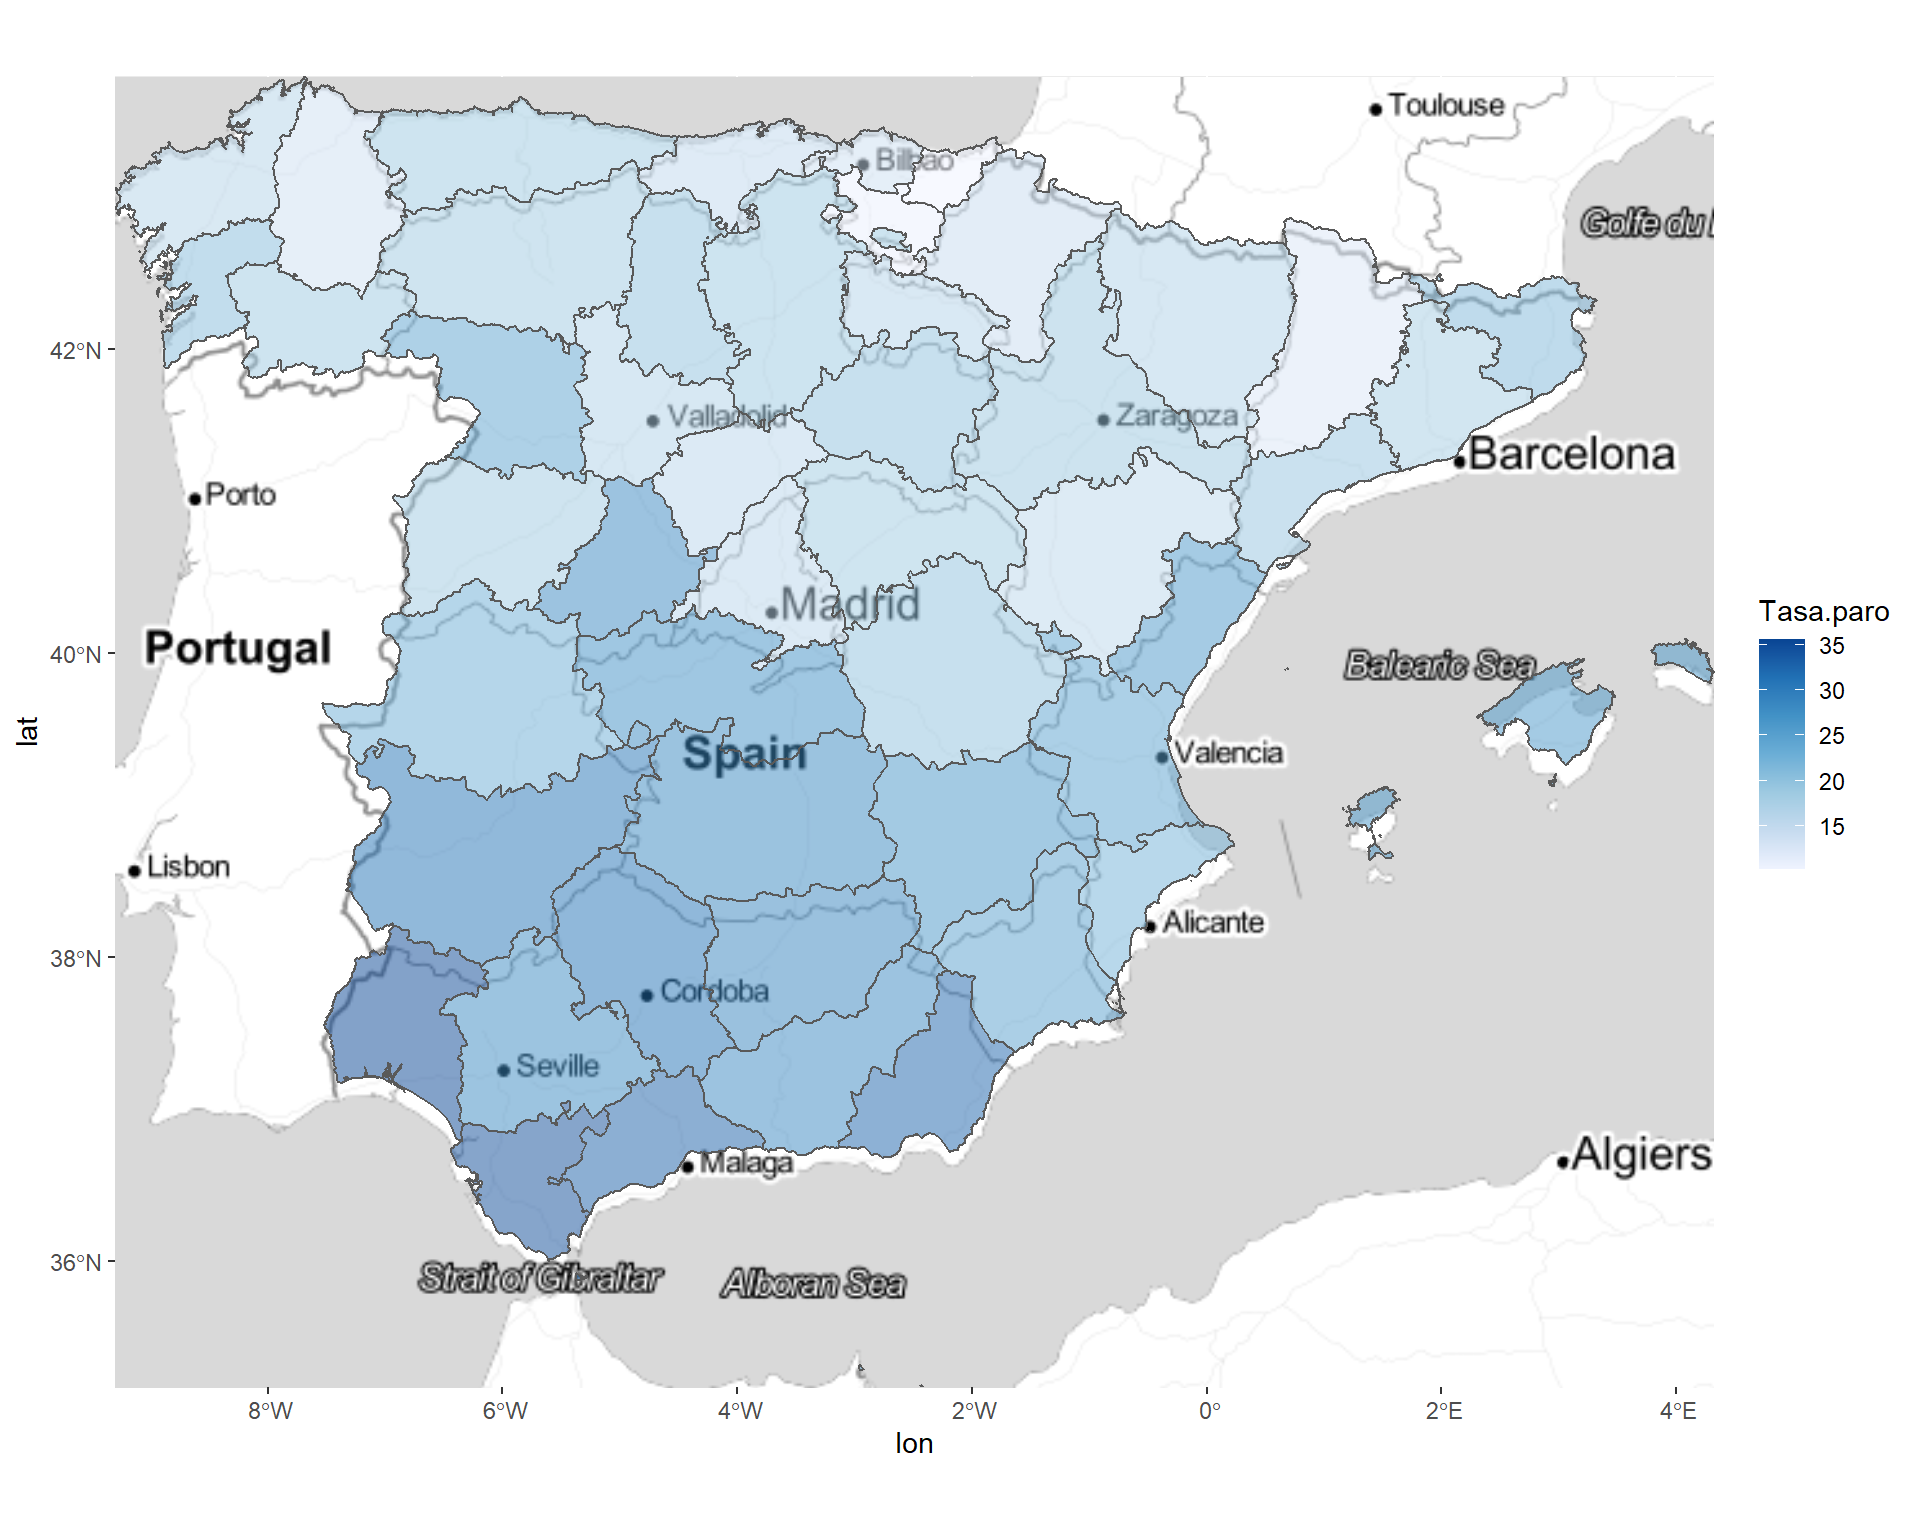
\includegraphics{graficosConR_files/figure-latex/unnamed-chunk-82-1.pdf}

\begin{Shaded}
\begin{Highlighting}[]
\NormalTok{code}\OtherTok{=}\StringTok{"ggtree(arbol, aes(color=group)) + geom\_tiplab(size=2)"}
\ControlFlowTok{for}\NormalTok{(i }\ControlFlowTok{in} \DecValTok{1}\SpecialCharTok{:}\DecValTok{6}\NormalTok{)\{}
\NormalTok{  mas}\OtherTok{=}\FunctionTok{paste0}\NormalTok{(}\StringTok{"geom\_cladelabel("}\NormalTok{,nodos[i],}\StringTok{",\textquotesingle{}"}\NormalTok{,familias[i],}\StringTok{"\textquotesingle{},offset=25, barsize=2,offset.text=2.5, fontsize=2, hjust=.2)"}\NormalTok{)}
\NormalTok{  code}\OtherTok{=}\FunctionTok{paste}\NormalTok{(code,mas,}\AttributeTok{sep=}\StringTok{"+"}\NormalTok{)}
\NormalTok{  \}}
\FunctionTok{eval}\NormalTok{(}\FunctionTok{parse}\NormalTok{(}\AttributeTok{text=}\NormalTok{code))}
\end{Highlighting}
\end{Shaded}

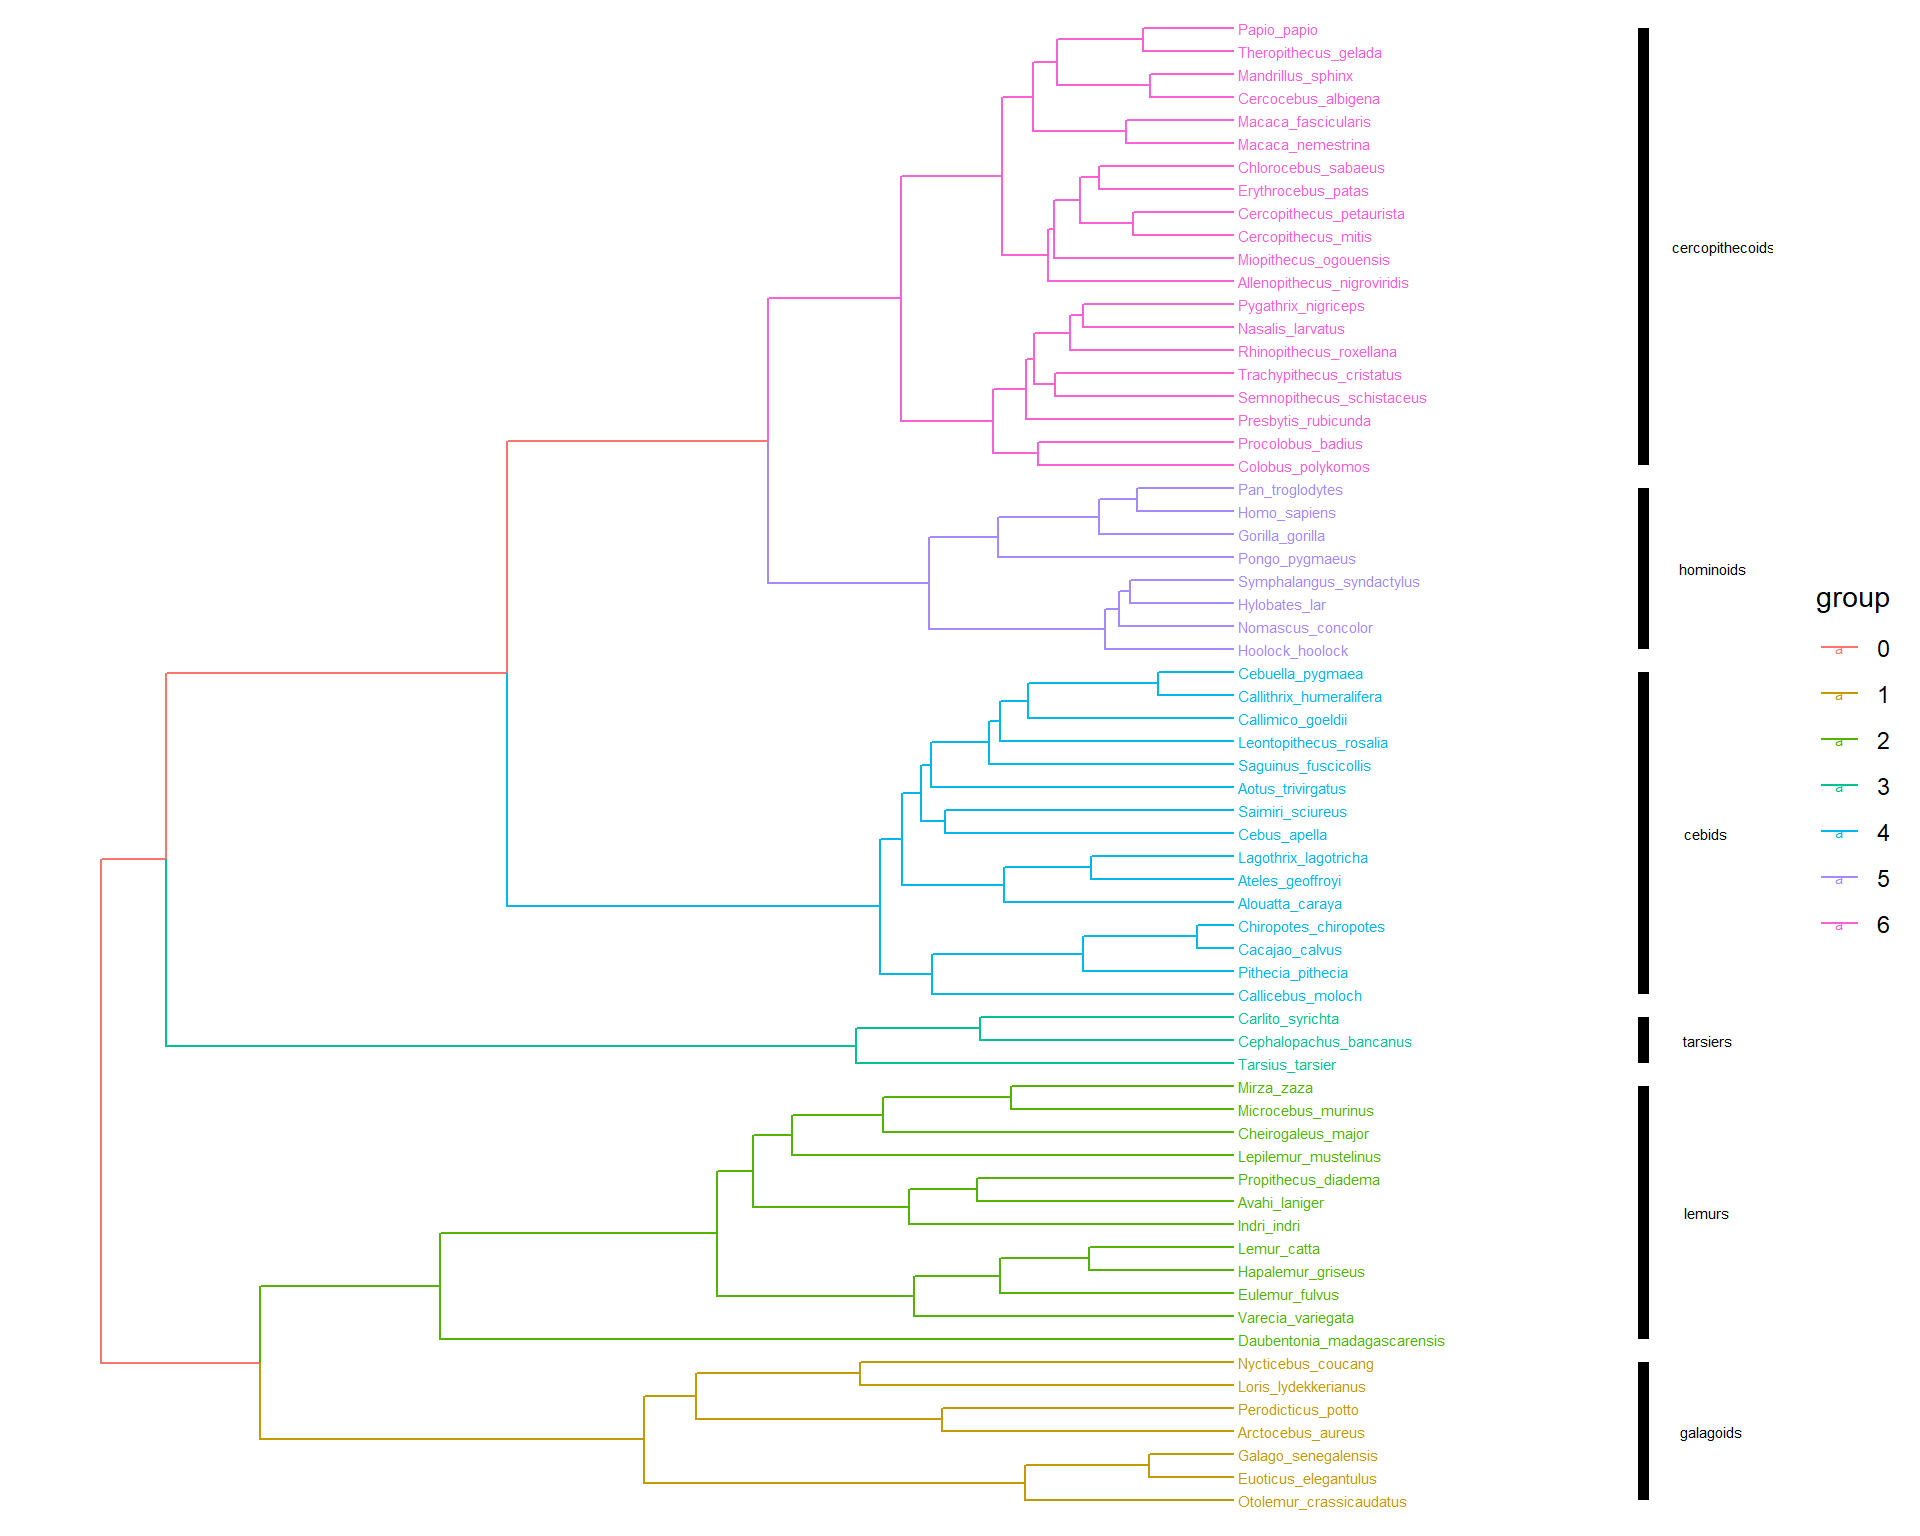
\includegraphics{graficosConR_files/figure-latex/unnamed-chunk-83-1.pdf}

\begin{Shaded}
\begin{Highlighting}[]
\DocumentationTok{\#\#\#\#\# Explorar la estructura de los siguientes arboles}
\NormalTok{arbol}\OtherTok{\textless{}{-}}\FunctionTok{read.tree}\NormalTok{(}\StringTok{"http://www.phytools.org/eqg2015/data/anole.tre"}\NormalTok{) }\CommentTok{\#filogenia de lagartijas}
\NormalTok{arbol }\OtherTok{\textless{}{-}} \FunctionTok{read.nexus}\NormalTok{(}\StringTok{"https://raw.githubusercontent.com/rgriff23/Dissertation/master/Chapter\_2/data/tree.nex"}\NormalTok{) }\CommentTok{\#filogenia de primates}
\end{Highlighting}
\end{Shaded}

\hypertarget{auxf1adir-heatmap}{%
\subsubsection{Añadir Heatmap}\label{auxf1adir-heatmap}}

Simulamos cinco caracteres continuos (ejemplo: tamaño del cuerpo, \ldots) de acuerdo al árbol filogenia:

\begin{Shaded}
\begin{Highlighting}[]
\FunctionTok{require}\NormalTok{(phytools)}
\FunctionTok{set.seed}\NormalTok{(}\DecValTok{1234}\NormalTok{) }\CommentTok{\# simulacion reproducible}
\NormalTok{traits }\OtherTok{\textless{}{-}} \FunctionTok{data.frame}\NormalTok{(}\FunctionTok{fastBM}\NormalTok{(arbol, }\AttributeTok{nsim=}\DecValTok{5}\NormalTok{))}
\end{Highlighting}
\end{Shaded}

utilizando las función \texttt{gheatmap} para adjuntar un \emph{heatmap} a la representación del árbol:

\begin{Shaded}
\begin{Highlighting}[]
\NormalTok{p }\OtherTok{\textless{}{-}} \FunctionTok{ggtree}\NormalTok{(arbol) }\SpecialCharTok{+} \FunctionTok{xlim}\NormalTok{(}\DecValTok{0}\NormalTok{, }\DecValTok{100}\NormalTok{) }\SpecialCharTok{+} \FunctionTok{geom\_tiplab}\NormalTok{(}\AttributeTok{size=}\DecValTok{2}\NormalTok{, }\AttributeTok{offset=}\DecValTok{17}\NormalTok{) }

\CommentTok{\# añade el heatmap}
\FunctionTok{gheatmap}\NormalTok{(p, traits, }\AttributeTok{offset=}\FloatTok{0.2}\NormalTok{, }\AttributeTok{width=}\FloatTok{0.2}\NormalTok{, }\AttributeTok{low=}\StringTok{"darkgreen"}\NormalTok{, }\AttributeTok{high=}\StringTok{"darkred"}\NormalTok{, }\AttributeTok{colnames\_position =} \StringTok{"top"}\NormalTok{, }\AttributeTok{font.size=}\DecValTok{2}\NormalTok{)}
\end{Highlighting}
\end{Shaded}

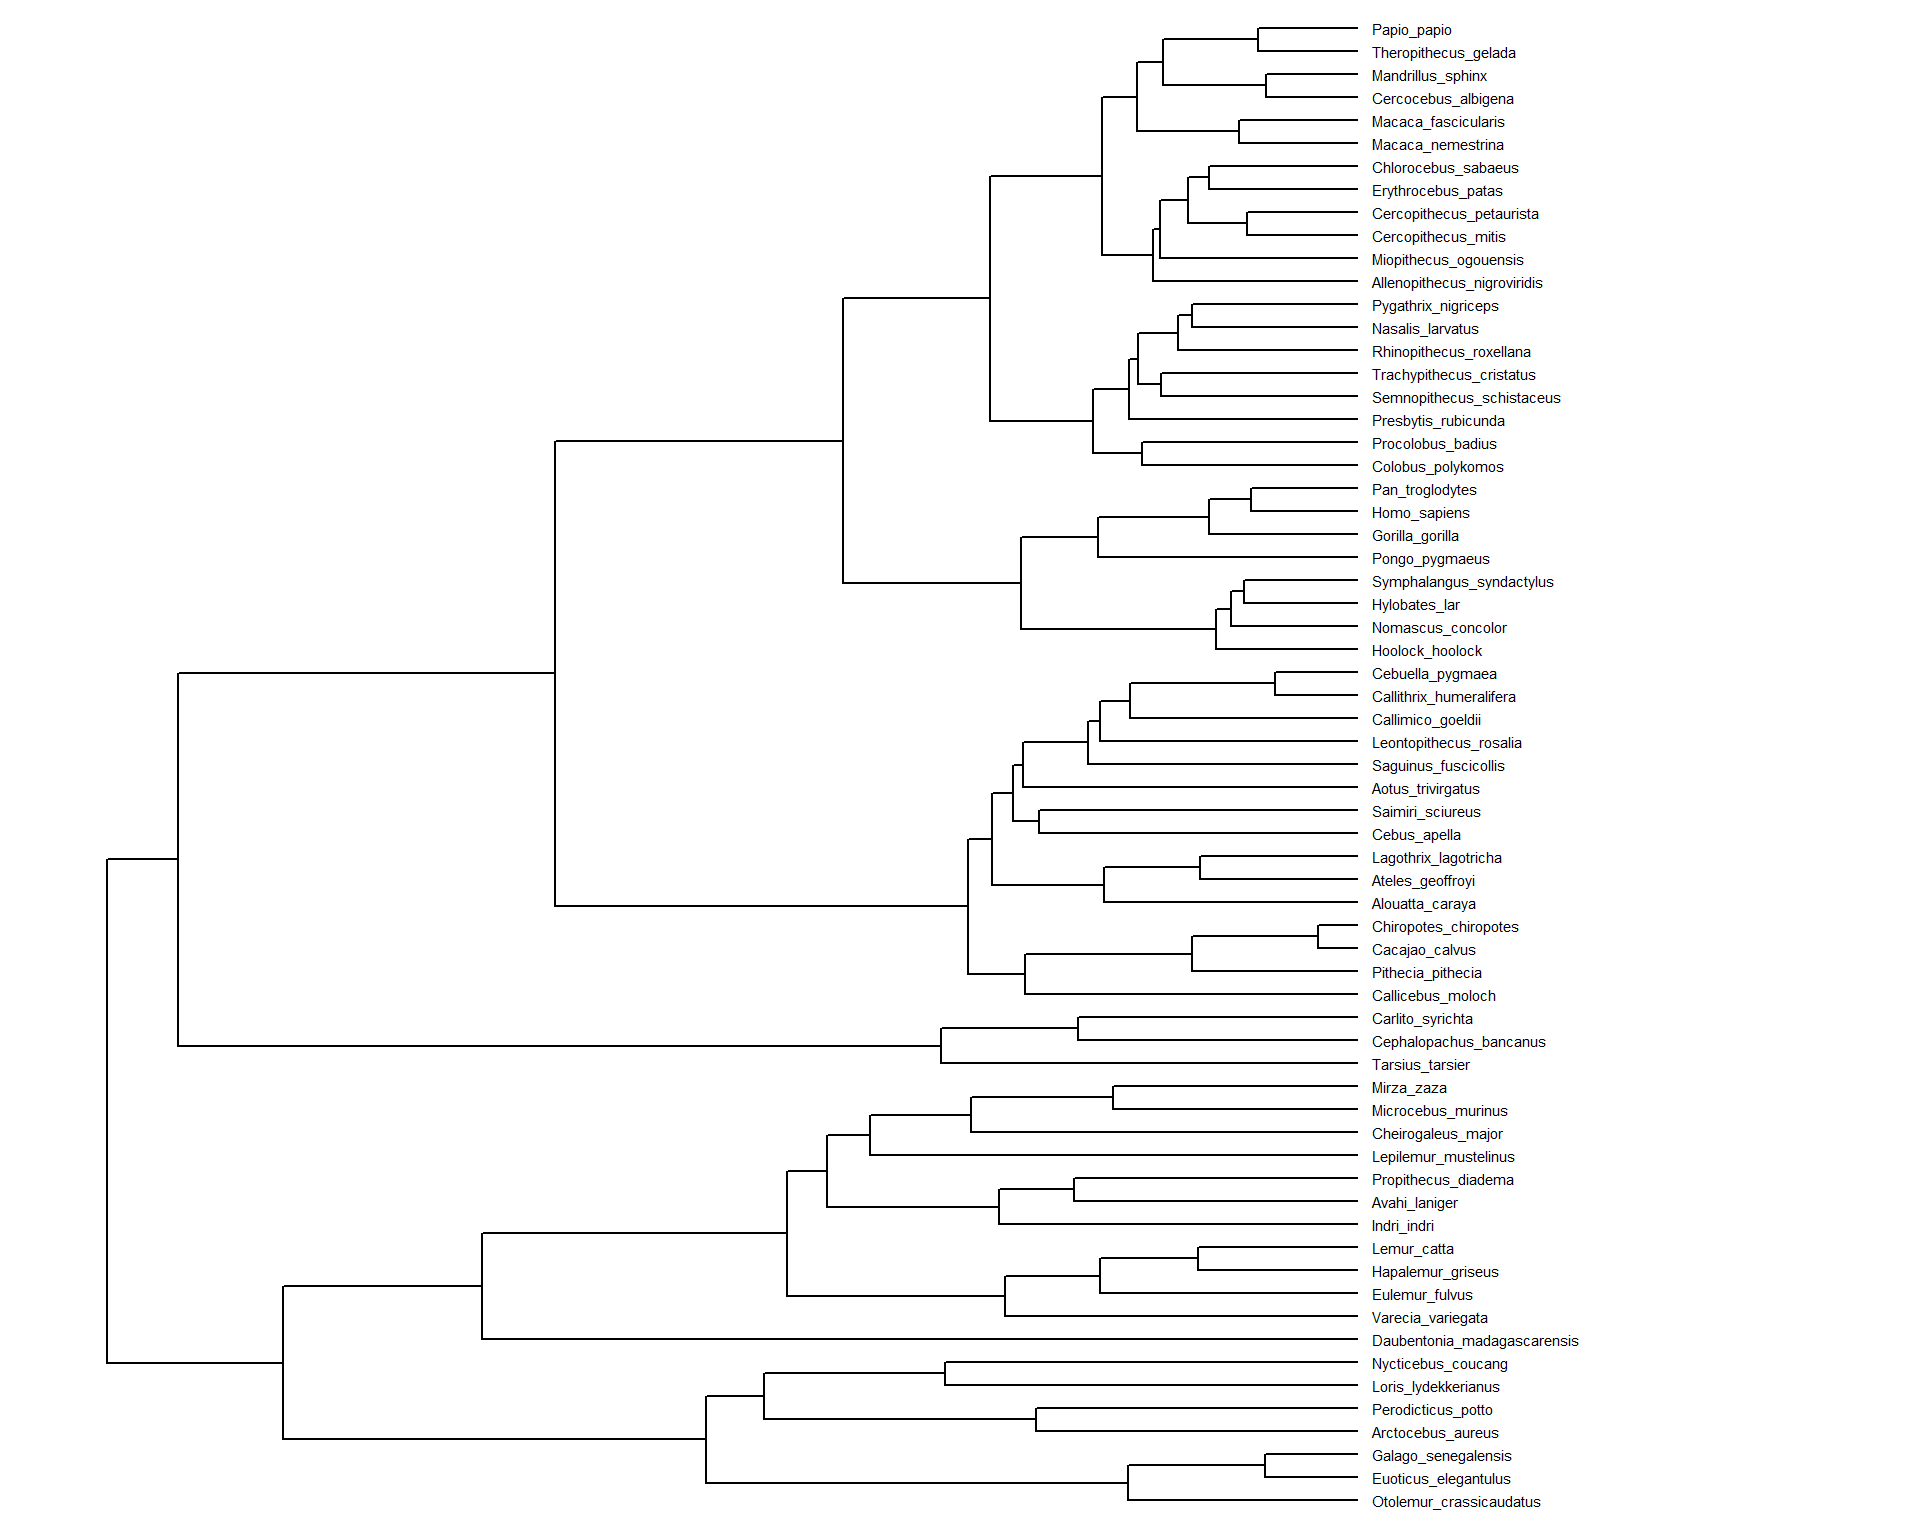
\includegraphics{graficosConR_files/figure-latex/unnamed-chunk-86-1.pdf}

\hypertarget{visualizaciuxf3n-de-multiple-arboles}{%
\subsubsection{Visualización de multiple arboles}\label{visualizaciuxf3n-de-multiple-arboles}}

\begin{Shaded}
\begin{Highlighting}[]
\NormalTok{trees }\OtherTok{\textless{}{-}} \FunctionTok{lapply}\NormalTok{(}\FunctionTok{c}\NormalTok{(}\DecValTok{10}\NormalTok{, }\DecValTok{20}\NormalTok{, }\DecValTok{40}\NormalTok{), rtree)}
\FunctionTok{class}\NormalTok{(trees) }\OtherTok{\textless{}{-}} \StringTok{"multiPhylo"}
\FunctionTok{ggtree}\NormalTok{(trees) }\SpecialCharTok{+} \FunctionTok{facet\_wrap}\NormalTok{(}\SpecialCharTok{\textasciitilde{}}\NormalTok{.id, }\AttributeTok{scale=}\StringTok{"free"}\NormalTok{) }\SpecialCharTok{+} \FunctionTok{geom\_tiplab}\NormalTok{(}\AttributeTok{size=}\DecValTok{2}\NormalTok{) }
\end{Highlighting}
\end{Shaded}

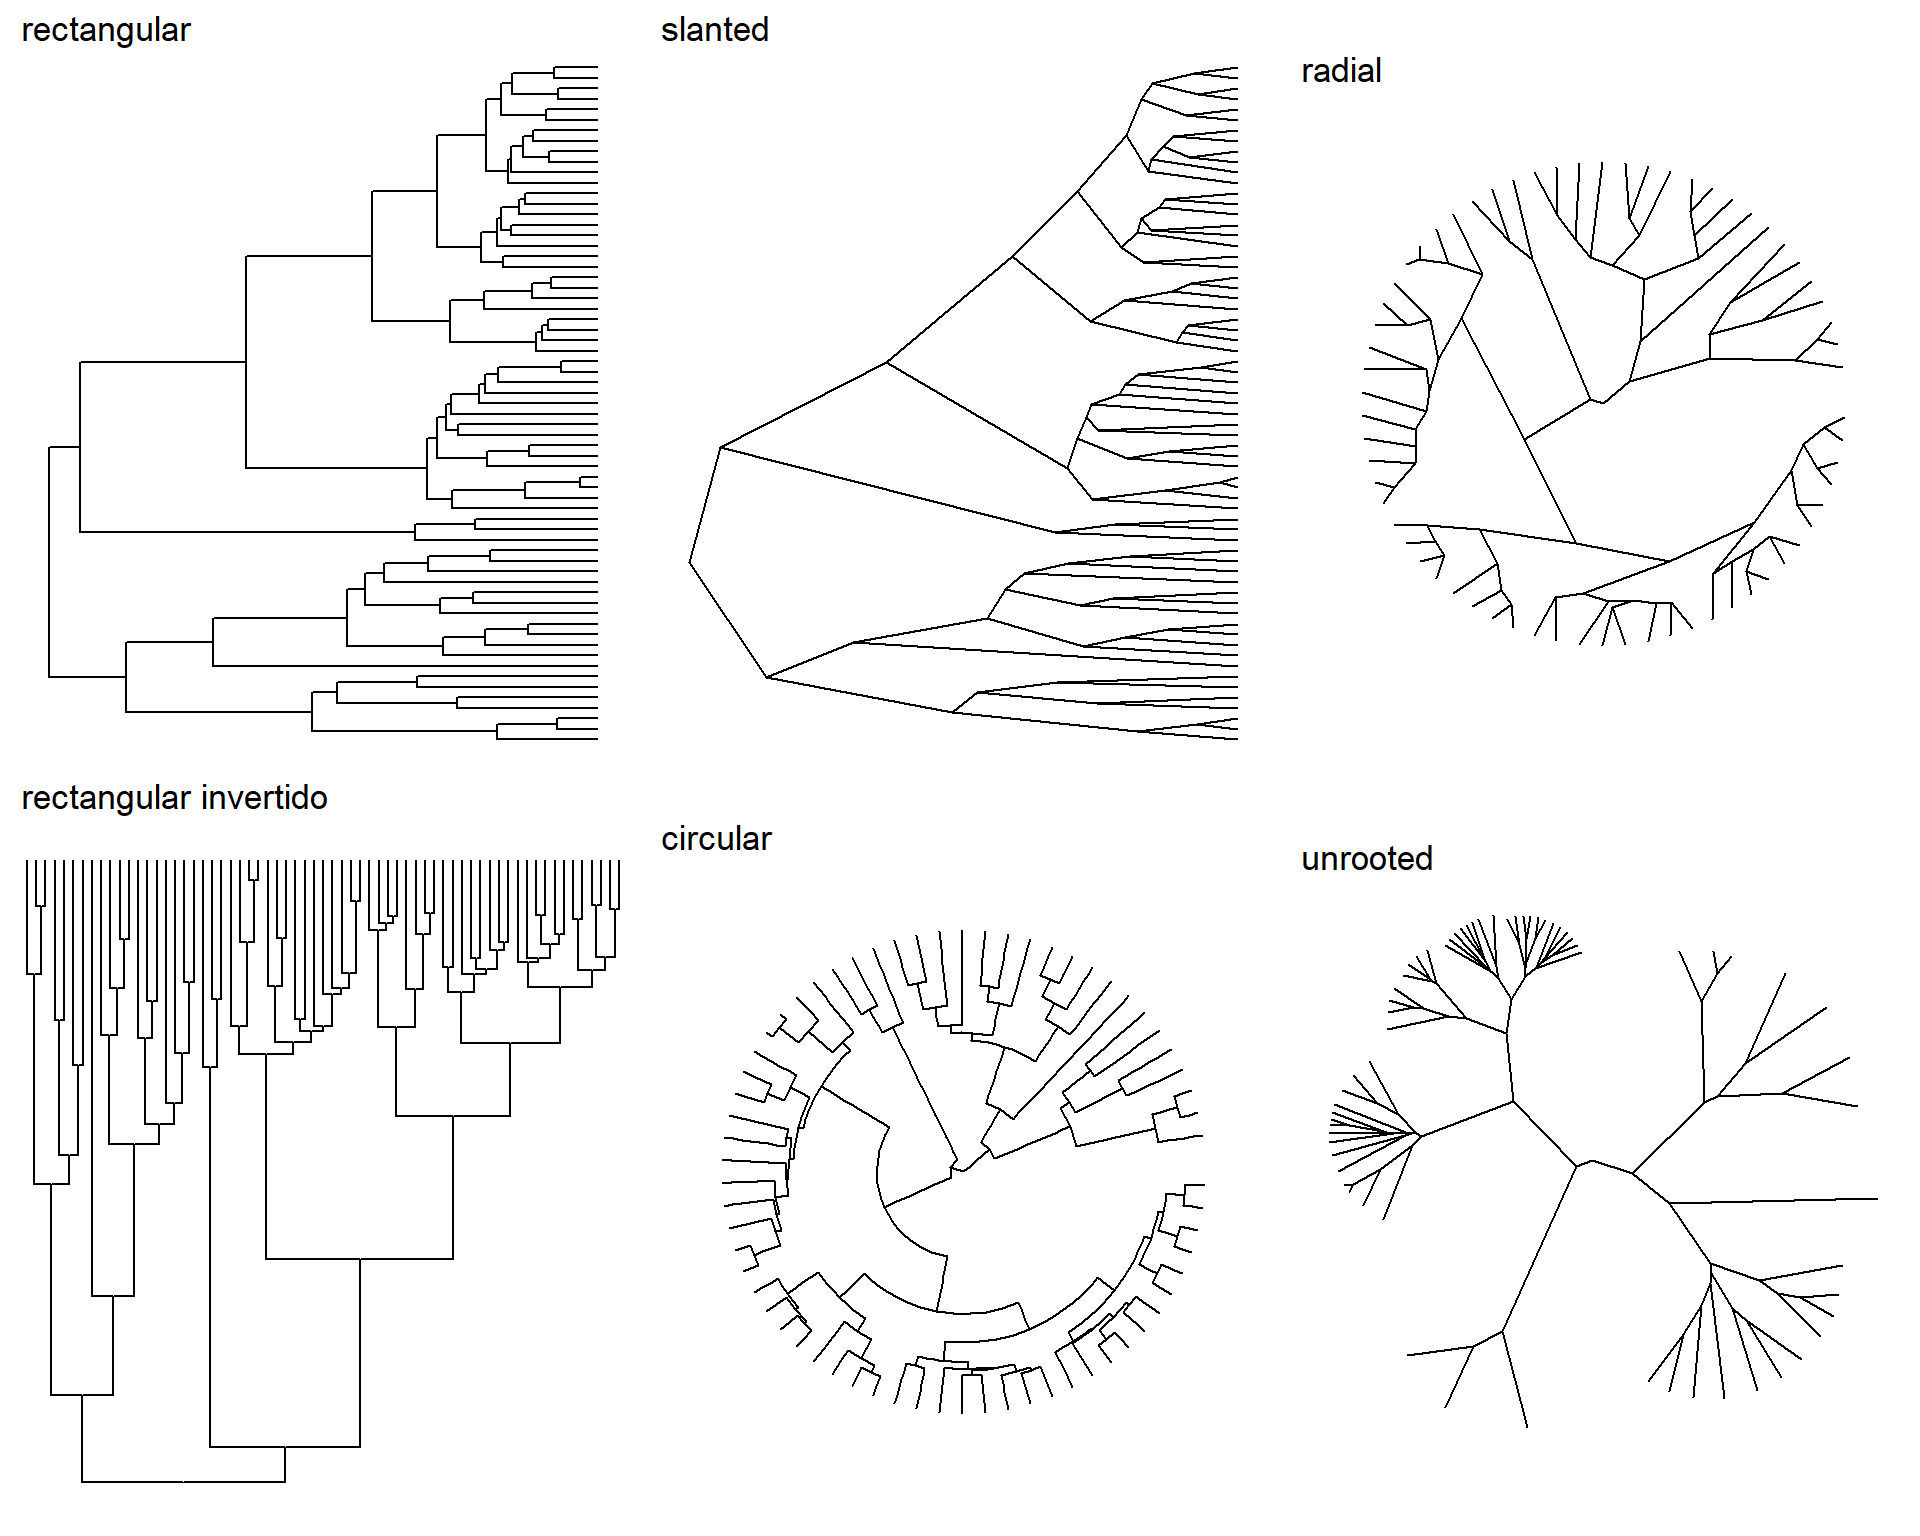
\includegraphics{graficosConR_files/figure-latex/unnamed-chunk-87-1.pdf}

\hypertarget{rmarkdown}{%
\section{Rmarkdown}\label{rmarkdown}}

Esta sección está dedicada a una extension de R: \texttt{rmarkdown}que permite crear documentos automatizados que combinan texto con código, tablas y gráficos generados directamente por R.

Este paquete no es complejo sino, más bien, extensos y llenos de detalles. El objetivo de esta sesión es recorrer sus posibilidades.

Rmarkdown permite generar documentos dinámicos al mezclar texto formateado y resultados generados por R. Los documentos generados pueden estar en HTML, PDF, Word y muchos otros formatos.

Las ventajas de esta herramienta son numerosas:

\begin{itemize}
\tightlist
\item
  El código y sus resultados no están separados de los comentarios asociados a ellos
\item
  El documento final es reproducible
\item
  El documento se puede actualizar fácilmente, por ejemplo, si los datos de origen se han modificado.
\end{itemize}

Por lo tanto, es una herramienta muy práctica para exportar, comunicar y difundir resultados estadísticos.

Este documento se ha generado a partir de archivos R Markdown \^{} {[}Más precisamente gracias a la extensión \texttt{bookdown} que permite generar documentos de tipo libro{]}.

Aprender Rmarkdown implica aprender dos cosas distintas:

\begin{itemize}
\tightlist
\item
  Markdown, un \emph{formato} para escribir documentos simples en modo texto. Tiene la ventaja de ser fácilmente legible por humanos pero, a la vez, procesable programáticamente para volcarlos en otros formatos: pdf, html, \ldots{}
\item
  La integración entre R y markdown
\end{itemize}

Aquí, un documento de R Markdown básico:

\begin{verbatim}
---
title: "Ejemplo de R Markdown"
output: pdf_document
---

*R Markdown* permite mezclar :

- texto libre puesto en formato
- bloques de codigo de R

Los bloques de codigo se pueden ejecutar para incluir sus resultados en el documento,
así por ejemplo :

```{r}
mean(airquality$Ozone,na.rm=TRUE)
```

## Gráficos

Se puede también incluir __gráficos__ :

```{r}
plot(Ozone~Temp,data=airquality,bg="lightblue",pch=21)
```
\end{verbatim}

Al ``compilar'' el documento, el texto se formatea, los bloques de código se ejecutan, sus resultados se agregan al documento y todo se transforma en uno de los diferentes formatos posibles (html, pdf, word, \ldots).

Aquí, la representación del documento anterior en formato HTML

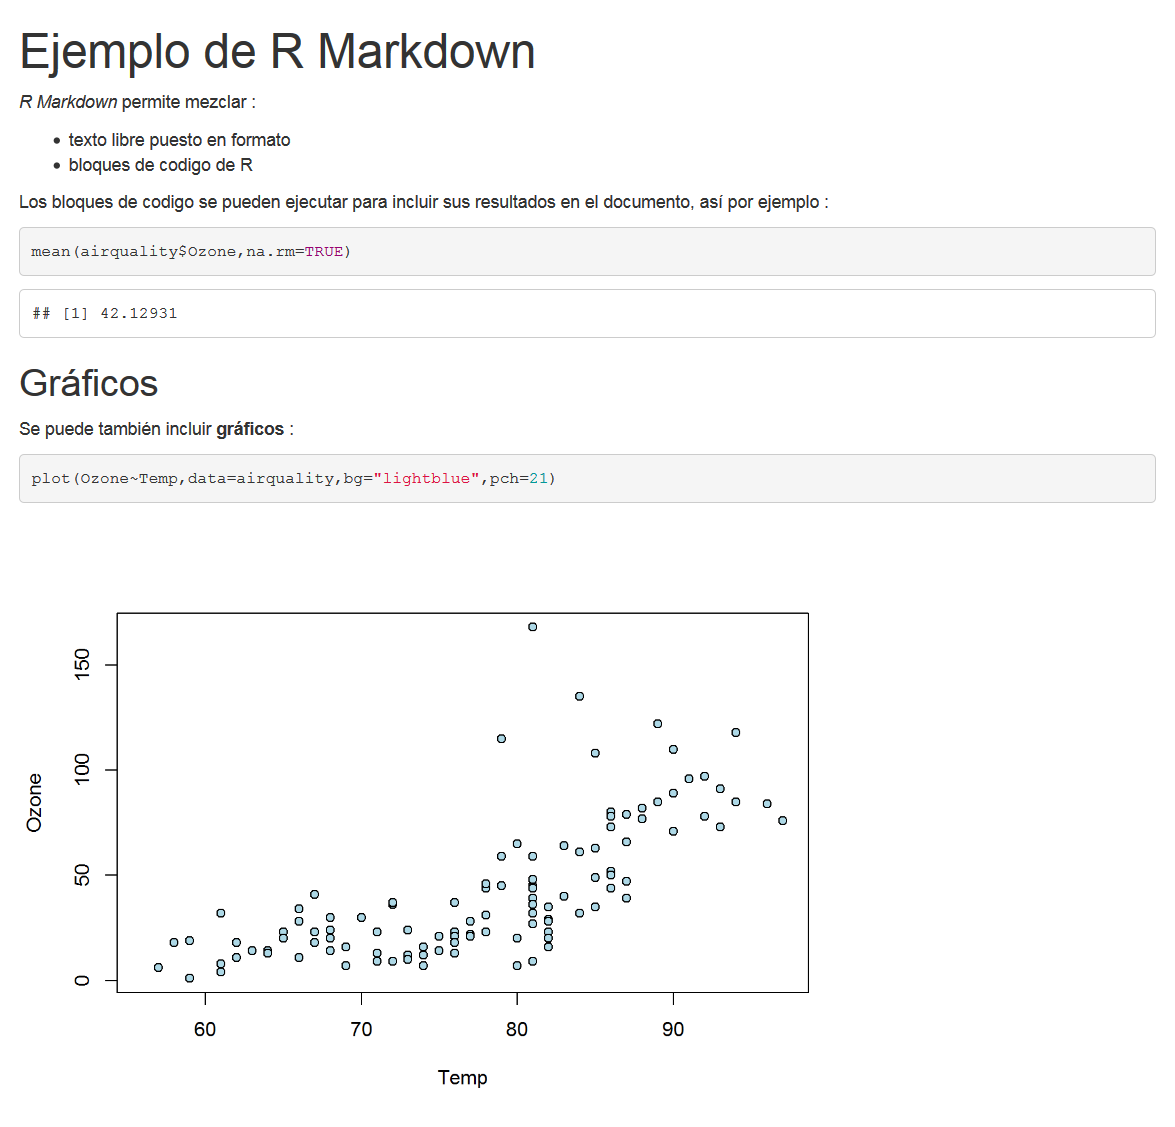
\includegraphics{resources/minimal.png}

\hypertarget{rmarkdown-en-15-mn}{%
\subsection{Rmarkdown en 15 mn}\label{rmarkdown-en-15-mn}}

Para aprender Markdown, se recomiendan los dos siguientes ejercicios :

\begin{ej}
Crear un fichero \texttt{.Rmd} usando
\texttt{File\ \textgreater{}\ New\ File\ \textgreater{}\ R\ Markdown}.
\end{ej}

Al crear un nuevo fichero de tipo \texttt{R\ Markdown}, RStudio proporciona, en lugar de uno vacío, una plantilla que muestra algunas de las opciones disponibles en este formato. Eso facilita el siguiente ejercicio:

\begin{ej}
Modificar el fichero de ejemplo creado en el ejercicio anterior
añadiéndole títulos de varios niveles, párrafos de texto, cursivas,
negritas, enlaces, listas (numeradas y sin numerar), etc. usando como
guía el
\href{https://www.rstudio.com/wp-content/uploads/2015/02/rmarkdown-cheatsheet.pdf}{\texttt{Cheat\ Sheet}}
del paquete. \emph{Compilar} el documento (p.e., pulsando el botón con
la etiqueta \emph{Knit HTML} situado encima del panel de edición de
RStudio) para inspeccionar el resultado final.
\end{ej}

Se puede también generar documentos en formato Word y PDF. Para estos formato, es necesario tener instalados los programas : MS Word, LibreOffice o similar para el primero y LaTeX para el segundo.

El segundo de los componentes de Rmarkdown (y lo que lo diferencia de Markdown \emph{a secas}) es la posibilidad de incorporar bloques de código en el hilo del documento. Estos bloques de código se procesan durante la compilación del documento y los resultados que generan (tablas, gráficos, etc.) se integran en la salida. La plantilla de fichero Rmarkdown que genera RStudio incluye unos cuantos ejemplos de bloques de código.

\begin{ej}
Insertar sobre el documento (o sobre una nueva plantilla) bloques de
código de R que hagan alguna cosa. Los bloques de código incluyen
opciones en su encabezamiento (p.e., para que un bloque se ejecute o no;
para que el código se muestre o se oculte en el documento final, etc.).
Las opciones disponibles se pueden consultar en el
\href{https://www.rstudio.com/wp-content/uploads/2015/02/rmarkdown-cheatsheet.pdf}{\texttt{Cheat\ Sheet}}
del paquete.
\end{ej}

\hypertarget{elementos-de-un-documento-rmarkdown}{%
\subsection{Elementos de un documento Rmarkdown}\label{elementos-de-un-documento-rmarkdown}}

\hypertarget{encabezado-pruxe9ambulo}{%
\subsubsection{Encabezado (préambulo)}\label{encabezado-pruxe9ambulo}}

La primera parte del documento es su \emph{encabezado}. Se encuentra al principio del documento y está delimitado por tres guiones (\texttt{-\/-\/-}) antes y después:

\begin{verbatim}
---
title: "Titulo"
author: "Nombre Apellido"
date: "2 de mayo de 2018"
output: html_document
---
\end{verbatim}

Este encabezado contiene los metadatos del documento, como su título, autor, fecha, más una serie de opciones posibles que permiten configurar o personalizar todo el documento y su representación. Aquí, por ejemplo, la línea \texttt{output:\ html\_document} indica que el documento generado tendrá un formato HTML.

\hypertarget{texto-del-documento}{%
\subsubsection{Texto del documento}\label{texto-del-documento}}

El cuerpo del documento consiste en texto con la sintaxis de Markdown: un marcado ligero que permite establecer niveles de títulos o formatear texto. Por ejemplo, el siguiente texto:

\begin{verbatim}
Este es un texto *en cursiva* y **en negrita**.

Se puede definir una lista así:

- primer elemento
- segundo elemento
\end{verbatim}

Que dará la siguiente salida

\begin{quote}
Este es un texto \emph{en cursiva} y \textbf{en negrita}.

Se puede definir una lista así:

\begin{itemize}
\tightlist
\item
  primer elemento
\item
  segundo elemento
\end{itemize}
\end{quote}

Los títulos de diferentes niveles se pueden definir comenzando una línea con uno o más caracteres \texttt{\#}:

\begin{verbatim}
# Titulo de nivel 1

## Titulo de nivel 2

### Titulo de nivel 3
\end{verbatim}

Cuando se han definido los títulos, al hacer clic en el icono \emph{Show document outline} en el extremo derecho de la barra de herramientas asociada al archivo, se muestra una tabla dinámica de contenidos generada automáticamente a partir de los títulos que permite navegar fácilmente en el documento.

La sintaxis de Markdown permite también insertar enlaces o imágenes. Por ejemplo, la siguiente sintaxis:

\begin{verbatim}
[ISCIII](http://www.isciii.es/)
\end{verbatim}

Dará el siguiente vinculo:

\begin{quote}
\href{http://www.isciii.es/}{ISCIII}
\end{quote}

En RStudio, el menú \emph{Help} y luego \emph{Markdown quick reference} proporciona una descripción más completa de la sintaxis.

\hypertarget{bloques-de-codigo}{%
\subsubsection{Bloques de codigo}\label{bloques-de-codigo}}

Además del texto libre en formato Markdown, un documento R Markdown contiene, como su nombre indica, código R. Este código se incluye en fragmentos definidos por la siguiente sintaxis:

Como esta cadena de caracteres no es muy fácil de escribir, se puede usar \emph{R} en el menú Insertar de RStudio, o teclear el atajo \texttt{Ctrl+Alt+i}.

Se puede dar un nombre al bloque y se indica directamente después de \texttt{r}:

\texttt{\{r\ nombre\_del\_bloque\}}

No es obligatorio, pero puede ser útil en caso de error de compilación, para identificar el bloque que causó el problema. Atención, no podemos tener dos bloques con el mismo nombre.

Además de un nombre, se puede pasar a un bloque una serie de opciones para modificar su comportamiento.

\begin{verbatim}
```{r echo = FALSE, warning = FALSE}
x <- 1:5
```
\end{verbatim}

Una de las opciones más útiles es la opción \texttt{echo}. Por defecto \texttt{echo=TRUE}, y el bloque de código R se inserta en el documento generado:

\begin{Shaded}
\begin{Highlighting}[]
\NormalTok{x }\OtherTok{\textless{}{-}} \DecValTok{1}\SpecialCharTok{:}\DecValTok{5}
\FunctionTok{print}\NormalTok{(x)}
\end{Highlighting}
\end{Shaded}

\begin{verbatim}
## [1] 1 2 3 4 5
\end{verbatim}

Pero, si la opción \texttt{echo=FALSE}, entonces el código R ya no se inserta en el documento, y solo se el resultado será visible:

\begin{verbatim}
## [1] 1 2 3 4 5
\end{verbatim}

Aquí hay una lista de algunas de las opciones más comunes:

\begin{longtable}[]{@{}lll@{}}
\toprule
opción & valores & descripción \\
\midrule
\endhead
echo & TRUE / FALSE & Mostrar o no el código R en el documento \\
eval & TRUE / FALSE & Ejecutar o no el código R en tiempo de compilación \\
warning & TRUE / FALSE & Mostrar o no las advertencias generadas por el bloque \\
message & TRUE / FALSE & Mostrar o no los mensajes generados por el bloque \\
\bottomrule
\end{longtable}

Hay muchas otras opciones descritas en la \href{https://www.rstudio.com/wp-content/uploads/2015/03/rmarkdown-reference.pdf}{Guía de referencia de R Markdown}.

\hypertarget{tablas-con-rmarkdown}{%
\subsection{Tablas con Rmarkdown}\label{tablas-con-rmarkdown}}

\hypertarget{tablas-cruzadas}{%
\subsubsection{Tablas cruzadas}\label{tablas-cruzadas}}

Por defecto, las tablas generadas por la función \texttt{table} se muestran tal y como aparecen en la consola de R, es decir, en texto sin formato:

\begin{Shaded}
\begin{Highlighting}[]
\CommentTok{\# titanic\textless{}{-}ftable(Survived\textasciitilde{}Class,data=Titanic)}
\CommentTok{\# Supervivencia al Titanic según clase}
\NormalTok{titanic}\OtherTok{\textless{}{-}}\FunctionTok{apply}\NormalTok{(Titanic,}\FunctionTok{c}\NormalTok{(}\DecValTok{1}\NormalTok{,}\DecValTok{4}\NormalTok{),sum)}
\NormalTok{titanic}
\end{Highlighting}
\end{Shaded}

\begin{verbatim}
##       Survived
## Class   No Yes
##   1st  122 203
##   2nd  167 118
##   3rd  528 178
##   Crew 673 212
\end{verbatim}

Su presentación se puede mejorar utilizando la función \texttt{kable} de la extensión \texttt{knitr}:

\begin{Shaded}
\begin{Highlighting}[]
\FunctionTok{library}\NormalTok{(knitr)}
\FunctionTok{kable}\NormalTok{(titanic,}\AttributeTok{caption=}\StringTok{"Supervivencia a la catastrofe del Titanic según la clase"}\NormalTok{)}
\end{Highlighting}
\end{Shaded}

\begin{table}

\caption{\label{tab:unnamed-chunk-96}Supervivencia a la catastrofe del Titanic según la clase}
\centering
\begin{tabular}[t]{l|r|r}
\hline
  & No & Yes\\
\hline
1st & 122 & 203\\
\hline
2nd & 167 & 118\\
\hline
3rd & 528 & 178\\
\hline
Crew & 673 & 212\\
\hline
\end{tabular}
\end{table}

\hypertarget{base-de-datos}{%
\subsubsection{Base de datos}\label{base-de-datos}}

Respecto a las bases de datos (\texttt{tibble} o \texttt{data.frame}), la presentación HTML por defecto es el contenido que aparece en consola. Este formato puede ser poco adecuado si la tabla excede una cierta dimensión.

Una alternativa es usar la función \texttt{paged\_table}, que muestra una representación HTML paginada de la base:

\begin{Shaded}
\begin{Highlighting}[]
\FunctionTok{require}\NormalTok{(gapminder)}
\NormalTok{rmarkdown}\SpecialCharTok{::}\FunctionTok{paged\_table}\NormalTok{(gapminder)}
\end{Highlighting}
\end{Shaded}

Otra alternativa es la función \texttt{datatable} de la extensión \texttt{DT}, que ofrece aún más interactividad:

\begin{Shaded}
\begin{Highlighting}[]
\FunctionTok{library}\NormalTok{(DT)}
\FunctionTok{datatable}\NormalTok{(gapminder)}
\end{Highlighting}
\end{Shaded}

En cualquier caso, no es recomendable mostrar una tabla de datos muy grandes de esta manera porque el archivo HTML resultante contendría todos los datos y, por lo tanto, sería muy grande.

\hypertarget{resumenes-de-base-de-datos}{%
\subsubsection{Resumenes de base de datos}\label{resumenes-de-base-de-datos}}

El paquete \texttt{gtsummary} permite generar automáticamente resúmenes de base de datos (la Tabla 1 en los artículos de epi) en un documento de Rmarkdown.

\begin{Shaded}
\begin{Highlighting}[]
\FunctionTok{require}\NormalTok{(gtsummary)}
\NormalTok{temp }\OtherTok{\textless{}{-}} \FunctionTok{subset}\NormalTok{(gapminder, }\AttributeTok{select=}\FunctionTok{c}\NormalTok{(continent,lifeExp, gdpPercap)) }
\FunctionTok{tbl\_summary}\NormalTok{(temp, }\AttributeTok{by=}\NormalTok{continent)}
\end{Highlighting}
\end{Shaded}

\begin{tabular}{l|c|c|c|c|c}
\hline
**Characteristic** & **Africa**, N = 624 & **Americas**, N = 300 & **Asia**, N = 396 & **Europe**, N = 360 & **Oceania**, N = 24\\
\hline
lifeExp & 48 (42, 54) & 67 (58, 72) & 62 (51, 70) & 72 (70, 75) & 74 (71, 78)\\
\hline
gdpPercap & 1,192 (761, 2,377) & 5,466 (3,428, 7,830) & 2,647 (1,057, 8,549) & 12,082 (7,213, 20,461) & 17,983 (14,142, 22,214)\\
\hline
\end{tabular}

Este mismo paquete permite también elaborar de manera eficiente tablas de resultados de regresión:

\begin{Shaded}
\begin{Highlighting}[]
\NormalTok{fit }\OtherTok{=} \FunctionTok{lm}\NormalTok{(lifeExp }\SpecialCharTok{\textasciitilde{}}\NormalTok{ continent,}\AttributeTok{data=}\NormalTok{gapminder)}
\NormalTok{T1 }\OtherTok{=} \FunctionTok{tbl\_regression}\NormalTok{(fit)}
\NormalTok{T1}
\end{Highlighting}
\end{Shaded}

\begin{tabular}{l|c|c|c}
\hline
**Characteristic** & **Beta** & **95\% CI** & **p-value**\\
\hline
continent &  &  & \\
\hline
Africa & — & — & \\
\hline
Americas & 16 & 15, 17 & <0.001\\
\hline
Asia & 11 & 10, 12 & <0.001\\
\hline
Europe & 23 & 22, 24 & <0.001\\
\hline
Oceania & 25 & 22, 29 & <0.001\\
\hline
\end{tabular}

\begin{Shaded}
\begin{Highlighting}[]
\NormalTok{fit2 }\OtherTok{=} \FunctionTok{lm}\NormalTok{(lifeExp }\SpecialCharTok{\textasciitilde{}} \FunctionTok{log}\NormalTok{(gdpPercap,}\DecValTok{2}\NormalTok{) }\SpecialCharTok{+}\NormalTok{ continent,}\AttributeTok{data=}\NormalTok{gapminder)}
\NormalTok{T2 }\OtherTok{=} \FunctionTok{tbl\_regression}\NormalTok{(fit2)}
\FunctionTok{tbl\_merge}\NormalTok{(}\FunctionTok{list}\NormalTok{(T1,T2),}\FunctionTok{c}\NormalTok{(}\StringTok{"Efectos crudos"}\NormalTok{,}\StringTok{"Efectos ajustados"}\NormalTok{))}
\end{Highlighting}
\end{Shaded}

\begin{tabular}{l|c|c|c|c|c|c}
\hline
**Characteristic** & **Beta** & **95\% CI** & **p-value** & **Beta** & **95\% CI** & **p-value**\\
\hline
continent &  &  &  &  &  & \\
\hline
Africa & — & — &  & — & — & \\
\hline
Americas & 16 & 15, 17 & <0.001 & 7.0 & 5.9, 8.1 & <0.001\\
\hline
Asia & 11 & 10, 12 & <0.001 & 5.9 & 5.0, 6.8 & <0.001\\
\hline
Europe & 23 & 22, 24 & <0.001 & 9.6 & 8.4, 11 & <0.001\\
\hline
Oceania & 25 & 22, 29 & <0.001 & 9.2 & 6.2, 12 & <0.001\\
\hline
log(gdpPercap, 2) &  &  &  & 4.5 & 4.2, 4.7 & <0.001\\
\hline
\end{tabular}

\hypertarget{referencias}{%
\section{Referencias}\label{referencias}}

Este curso está basado en las siguientes referencias:

\begin{itemize}
\item
  \emph{R para profesionales de los datos}, Carlos Bellosta, 2017,
  \href{https://datanalytics.com/libro_r}{\texttt{https://datanalytics.com/libro\_r}}
\item
  El libro \href{http://r4ds.had.co.nz/r-markdown.html}{R for data science} disponible en línea, que contiene un capítulo dedicado a R Markdown .
\end{itemize}

Y también muy inspirado de estos otros libros:

\begin{itemize}
\item
  \emph{Data Visualisation with R}, Thomas Rahlf, 2014, \href{http://www.datavisualisation-r.com/}{\texttt{http://www.datavisualisation-r.com/}}
\item
  \emph{R Graph Cookbook} , Hrishi Mittal, 2011
\end{itemize}

\end{document}
